\documentclass{vldb}
%\paperwidth=8.5in
%\paperheight=11in
%\usepackage[margin=1in]{geometry}

\usepackage{amsmath,amsfonts,amssymb}
\usepackage{color}
\usepackage{graphicx}
\usepackage{epsfig}
\usepackage{url}
\usepackage{semantic}
\usepackage{subfigure}
\newcommand{\figref}[1]{Figure \ref{#1}}
\newcommand{\tabref}[1]{Table \ref{#1}}
\newcommand{\eqnref}[1]{Equation \ref{#1}}
\newcommand{\KZ}[1]{\textcolor{blue}{(KZ: #1)}}
\newcommand{\ZY}[1]{\textcolor{red}{(#1)}}
\newcommand{\ERIC}[1]{\textcolor{green}{(Eric: #1)}}
\newcommand{\cut}[1]{}
\newcommand{\dd}[0]{\mathrm{d}}
\newcommand{\numberthis}{\stepcounter{equation}\tag{\theequation}}

\usepackage{courier}
\usepackage{listings}
\lstset{ %
	numberstyle=\scriptsize,
	basicstyle=\scriptsize\ttfamily,
	breaklines=true,
	tabsize=1,
	columns=fullflexible,
	numbers=left,
	stepnumber=1
}



\DeclareMathOperator*{\var}{var}
\DeclareMathOperator*{\val}{val}
\DeclareMathOperator*{\dom}{dom}

\mathlig{=>}{\Rightarrow}
\mathlig{->}{\rightarrow}

\newcounter{enum}
\newenvironment{packed_enum}{
%\begin{list}{\arabic{enum}.}{
\begin{list}{(\alph{enum})}{
  \setlength{\itemsep}{-0.5pt}
  \setlength{\parskip}{1pt}
  \setlength{\labelwidth}{30 pt}
  \setlength{\leftmargin}{15 pt}
  \setlength{\itemindent}{0pt}
  \usecounter{enum}}
}{\end{list}}


\makeatletter
\newcommand{\Spvek}[2][r]{%
  \gdef\@VORNE{1}
  \left(\hskip-\arraycolsep%
    \begin{array}{#1}\vekSp@lten{#2}\end{array}%
  \hskip-\arraycolsep\right)}

\def\vekSp@lten#1{\xvekSp@lten#1;vekL@stLine;}
\def\vekL@stLine{vekL@stLine}
\def\xvekSp@lten#1;{\def\temp{#1}%
  \ifx\temp\vekL@stLine
  \else
    \ifnum\@VORNE=1\gdef\@VORNE{0}
    \else\@arraycr\fi%
    #1%
    \expandafter\xvekSp@lten
  \fi}
\makeatother

\newcommand\Mark[1]{\textsuperscript{#1}}

\begin{document}
%\pagestyle{empty}

\title{Declarative Bayesian Inference on Spark}

\author{
Zhuoyue Zhao~\Mark{1}, Eric Lo~\Mark{2}, Kenny Q. Zhu~\Mark{1}, Chris Liu~\Mark{2}\\
\affaddr{
\Mark{1}Shanghai Jiao Tong University
\hspace*{5mm}\Mark{2}Hong Kong Polytechnic University}\\
\email{\{zzy7896321@, kzhu@cs.\}sjtu.edu.cn
\hspace*{2mm}\{ericlo, cscyliu\}@comp.polyu.edu.hk
}}

\maketitle

%\unitlength1pt
%\begin{picture}(0,0)
%\put(380,190){\mbox{\Large \bf  Paper \#478}}
%\end{picture}
%\unitlength1cm


\begin{abstract}
The Apache Spark stack has enabled fast
large-scale data processing.
Despite a rich library of statistical models and
inference algorithms, it does not give domain
users the ability to develop their own models.
The emergence of probabilistic programming languages 
has showed the promise of developing sophisticated
probabilistic models through succinct and declarative modeling.
%helps data analysts and machine learning experts to concisely 
%describe the probabilistic models using a programming language. 
These frameworks have the potential of automatically generating
inference algorithms for the user defined models and 
answering various statistical queries about the model. 
It is a perfect time to unite these two great directions to
produce a declarative big data analysis framework. 
We thus propose, InferSpark, a declarative Bayesian inference
framework on top of Apache Spark. 
Efficient Bayesian inference can be easily implemented on this 
framework and inference process can leverage the distributed 
main memory processing power of Spark. 
%This framework makes statistical inference on
%big data possible and speed up the penetration of probabilistic 
%programming into the data engineering domain. 
\end{abstract}

%\IEEEraisesectionheading{
% %\IEEEraisesectionheading{
% %\IEEEraisesectionheading{
% \input{intro}
\section{Introduction}\label{sec:intro}
 %}
% \section{Introduction}\label{sec:intro}

% \begin{enumerate}
% \item Motivation: application scenarios (with 1-2 running examples);
% \item Characteristics of the data sources and their challenges;
% \item Briefly introduce previous approaches to extract information 
% from images including setting the document zone, and their limitations.
% \item General flow of our approach (may give a diagram here)
% \end{enumerate}
% scenary

Due to ever evolving hardware and software, many medical images
such as electro-cardio graphs (ECGs), X-ray or ultrasound images  
are directly printed and stored in hard copy formats. 
% \KZ{Insert 4 example images here.}
%Examples are shown in \figref{fig:medicalImages}. 
% These images often contain a mix of graphics and text, which
% include parameter settings of the hardware, test measurements or simple
% diagnosis. 
These images often contain a mix of graphics and text, which 
include technical settings of the hardware used, test measurements or simple diagnoses.
Recently, there has been a growing demand for digitizing such 
medical information from paper media sources, especially legacy ones, or patients who want to keep track of these documents by themselves digitally. 
Apart from scanning the graphics into a digital format, extracting 
the semi-structured textual information is also an important part of
building electronic medical records for patients. 

%\begin{figure}[!htb]
%\centering
%\subfloat[ECG]{
%\label{fig:medicalimage:ecg}
%\epsfig{file=figure/17_ori.eps, width=0.4\columnwidth}
%}
%% \hfill
%\subfloat[MRI]{
%	\label{fig:medicalimage:mrt}
%	\epsfig{file=figure/MRI.eps, width=0.4\columnwidth}
%}
%\\
%\subfloat[X-RAY]{
%\label{fig:medicalimage:xray}
%\epsfig{file=figure/X-RAY.eps, width=0.4\columnwidth}
%}
%%\hfill
%\subfloat[EEG]{
%\label{fig:medicalimage:eeg}
%\epsfig{file=figure/EEG.eps, width=0.4\columnwidth}
%}
%\caption{Examples of Medical Images}
%\label{fig:medicalImages}
%\end{figure}

Optical character recognition (OCR)  \cite{mori1992historical,smith2007overview} is 
a traditional technique used to turn images of printed text into machine encoded
text. It is well researched and performs well on plain text 
documents such as novels and reports, for a variety of languages. 
%For example, Tesseract, which is one of 
%the most popular open source multilingual recognizers, logs an error 
%rate of 3.72\% for English words and 3.77\% for simplified 
%Chinese characters\cite{smith2009adapting}. 
%Google Books \cite{googlebooks} and Gutenberg \cite{gutenberg} are
%projects which have scanned a large number of paper books into text for free and open
%access. These projects made exclusive use of OCR for this conversion and 
%achieved high accuracy \cite{vincent2007google} \cite{lebert2008project}. 
% 99\% for Gutenberg project \cite{lebert2008project}. 
% \KZ{Give the accuracy of google and gutenberg if available.}


\begin{figure}[th]
\centering
\epsfig{file=figure/17_b.eps, width=0.8\columnwidth}
\caption{An ECG image with text area (red circle) of interest.}
\label{fig:ecgexample2}
\end{figure}

For a semi-structured medical image, such as 
\figref{fig:ecgexample2}, we would like to extract the attribute-value 
pairs (e.g., {\em Vent. rate = 63 bpm}) and possibly other values such as
date ({\em 18-Nov-2010}) and time ({\em 9:13:02}) since those values endow us with lots of information about the patient. 
Existing OCR software cannot extract such structured information in a straightforward 
fashion, 
but instead it produces rather convoluted results from the whole image, 
similar to those in \figref{fig:ocrre}, which was produced by Tesseract, 
a popular multi-lingual recognizers. 
% \KZ{Maybe include the x-y coordinate info in the output as well?}  

\begin{figure}[th]
\centering
\scriptsize
\begin{verbatim}
<p class="ocr_par" title="box 263 33 444 119">
   <span class="ocr_l" title="box 264 33 336 45">
       <span class="ocrx_w" title="box 264 33 299 45">Vcnt.</span> 
       <span class="ocrx_w" title="box 308 34 336 45">rule</span> 
   </span>
   <span class='ocr_l'>
       <span class="ocrx_w" title="box 264 51 283 64">PR</span> 
       <span class="ocrx_w" title="box 291 51 346 64">Interval</span> 
       <span class="ocrx_w" title="box 389 52 411 64">140</span> 
       <span class="ocrx_w" title="box 420 55 439 64">ms</span> 
   </span>
   ...
   </span>
</p>
<p class="ocr_p" dir="ltr">
   <span class="ocr_l">
       <span class="ocrx_w" title="box 396 33 411 45">53</span> 
       <span class="ocrx_w" title="box 420 33 449 48">bpm</span> 
   </span>
</p>
\end{verbatim}
\caption{Snippet OCR results in XML, input to our framework.}
\label{fig:ocrre}
\end{figure}


%\input{xmlre1}

%However, OCR alone does not work well on semi-structured text and hence
%can't be directly used for information extraction from the aforementioned
%medical images. \KZ{Give the reason here, perhaps because OCR models are
%largely Markov based? So semi-structured data breaks the flow of text.}
%When a medical image is input to an ordinary OCR software, the spatial 
%information of the text components is often lost or mixed with noises
%and errors.
%%The reason is OCR converts the whole images into text data, in which 
%%useful information often mix with noises and errors. 
%In this paper, we would like to extract the attribute-value pairs
%and possibly other values from \figref{fig:ecgexample1} 
%and \figref{fig:ecgexample2}. 
%% or medical ultrasonography report. 
%Such images contain lots of non-textual information or noises.

% example & ref
%\begin{figure}[ht]
%\centering
%\epsfig{file=figure/46.eps, width=0.8\columnwidth}
%\caption{ECG Images From Printer1}
%\label{fig:ecgexample1}
%\end{figure}

% \begin{figure}[ht]
% \centering
% \subfloat[Printer1]{
% \label{fig:ecgexample:a}
% \epsfig{file=figure/46.eps, width=0.48\columnwidth}
% }
% \hfill
% \subfloat[Printer2]{
% \label{fig:ecgexample:b}
% \epsfig{file=figure/17.eps, width=0.48\columnwidth}
% }
% \caption{ECG images from two different printers}
% \label{fig:ecgexample}
% \end{figure}

Also, errors in the OCR text \cite{darwish2007error,taghva1996evaluation} will greatly affect the effectiveness 
of other related tasks. Much work has been done to improve the performance of the OCR\cite{kolak2003generative,cesarini1998informys}. However, there are still a number of significant challenges involved in extracting the information from medical images or OCR results in XML form. 

% First, medical images differ from pure text document in that them have 
% layout information. 
First, medical images differ from pure text documents in that 
they contain layout information.
Although most current OCR engines attempt to reproduce the physical 
layout of the text units, 
%(along with X-Y coordinates) and store them 
%in a special format such as XML 
% (\KZ{Better in the previous example})
such spatial
information is approximate and sometimes inaccurate, which is why neighboring
text blocks in \figref{fig:ecgexample2}, such as ``Vent. Rate'' and
``63 bpm'' were not automatically combined into the same XML block, but were 
rather far apart (shown in two different ``classes'') in \figref{fig:ocrre} made by OCR softwares. 
%Even for images produced by the same ECG printer, 
%the XML results can still be very different as 
The spatial layout is sensitive to many factors, such as accidental spots 
on the prints, color and contrast, or the angle of the camera. 
%In this case, solutions for other application domains, for example, the web, 
%are not well suited for information extraction from printed documents \cite{bartoli2014semisupervised}. With such inaccurate
%layout information produced by OCR,
%it is not easy to write a simple wrapper program to extract useful
%data from images, even if the images come from the same printer. 

%Writing a wrapper for each
%individual image would be tedious and counter-productive. Therefore,
%a mechanism that makes use of the spatial locality of the 
%text units in the image and 
%accommodates slight variations in the spatial layout would make the extraction
%more accurate and fault-tolerant.

%For example, \figref{fig:ocrre} is the simplified OCR results for the ECGs in 
%\figref{fig:ecgexample1} and \figref{fig:ecgexample2}. The results are in the XML format and have attritube named {\em class} 
%for layout information. Although these two images share similar format. 
%OCR engine generates different results in that it splits elements that 
%should be in the same line into two lines in the second example. 
%XML is sensitive to the layout results so it's hard to tolerate 
%all the layout results. 
%
% example check the term
% layout of ocr results can be restore, so why OCR engine don't restore the results 
% using the similar methods as we do?
% or the way we handle the layout problem is quite simple

% Delete for TIP
% Second, exiting OCR engines make heavy use of Markov properties such as n-grams
% since they primarily target the transformation of large body of text 
% \cite{kolak2003generative}. 
% % \KZ{Needs some refs here.}
% Unfortunately, the semi-structured texts in medical images are often 
% short and not even written in complete sentences, thus breaking Markov assumption. To make
% matters worse, medical images contain scientific language, which may be
% very different from the training corpora of these OCR engines.
% This explains why we see errors like ``Vcnt'' and ``rule'' 
% in \figref{fig:ocrre}. 
% %can't guarantee a perfect performance, which means 
% %there are errors and noises in the OCR results.
% %Many of them due to the fact that the data are no longer long, continous
% %sentences, thus breaking the Markov assumption made by many OCR algorithms. 
% %In \figref{fig:ocrresub:b}, ``Vent." is misrecognized as ``Vcnt.". 
% Without sufficient contextual information, OCR may also misrecognize a 
% digit as an alphabetic character, or as another similar digit. 
% Furthermore, the mix of text with images and formatting
% lines often confuses the OCR engine, which is more biased toward full
% text images.
% Exact pattern matching, as used in
% traditional information extraction, doesn't work with such noisy OCR output
% as it doesn't tolerate noises or errors in text. 
% %It's hard to autocorrect these errors 
% %because image quality is the most important affecting factor. 
% %The text we are processing can be full of no meaning words or 
% %strange numbers. 
% A fuzzy matching strategy is more desirable in this case. 
% % example, what are the traditional IEs

Second, there are many types of medical images, resulting from a variety of
medical tests. Different equipments for the same test can produce vastly 
different images. Writing individual extraction wrappers 
for the OCR outputs of all these formats is tedious and inefficient, 
and difficult for non-programmers.
%not to mention that there are significant programming barriers for 
%writing these wrappers, especially for the medical professionals who are the
%end users of these extraction results. 
%A more user-friendly approach enabling users to specify such extraction requirements would be preferred. 
%There are various kinds of medical images, such as electrocardiograph report, 
%medical ultrasonography report, etc. 
%However the basic measures for each type of medical test (e.g., ECG), 
%are very similar from machine to machine. Only the layouts are 
%different. 
% example medical images

Finally, most off-the-shelf OCR programs are pre-trained with specific 
recognition models, which may not be suitable for the extraction of 
%medical images.
%Furthermore, changes in imaging equipment technology over time may produce 
%different formats, layout, or terminology, rendering existing OCR models 
%obsolete. 
Re-training the models requires a large amount of labeled data, which may
not be available. 
%Incremental training as more labeled data arrives
%is currently not supported by any OCR product.    

%There have been some limited attempts to address some of the above challenges. 
%One solution is a plugin of an OCR program that allows the user to specify 
%target zones of interest in the image to be extracted. The zones specified for
%one image can be applied to images with slight variations by adjusting against
%a fixed reference point that is supposed to exist in all these images.
%% \KZ{I think the problem is not so much with the zones, because we also
%% have zones, but rather with the reference point.}
%% \JY{}
%% example products
%% http://www.square-9.com/automated-data-extraction-optical-character-recognition
%The problem with this solution is its high reliance on the OCR zones  
%established by the user. The performance of the results is affected by the 
%accuracy of the zones. If the zones are too big, the results will be full of 
%noise. If the zones are too small, results will miss something. 
%
%Another solution involves using the page layout analysis technique. The page layout 
%analysis technique is used to determine where the text 
%resides on a page \cite{o1993document}, 
%% \KZ{This page layout analysis approach is not clearly described. I don't understand after reading this paragraph.}
%% By using page layout analysis technique, the hierarchy of physical components 
%% can be generated and to match with the hierarchy of logical components, which 
%% is predefined. 
%this includes identifying and categorizing the 
%regions of interest in the scanned image of a text document. 
%Typically, the first step is to segment text zones from 
%non-textual zones and arrange them in their original order. 
%Then in order to analyze the logical roles of the text zones 
%(titles, captions, footnotes, etc.), logical layout analysis 
%is used for labeling the semantics of the text zones.
%Generally, page layout analysis is used for documents. The problem with applying 
%such a technique on medical images is that it creates so much noises 
%that performance is ultimately affected. 
%For medical imaging reports like ECG, useful information is often 
%found in the small components of the image, while most of the images are 
%read as noises. 
% check paper and more description, weakness, ref

%In this paper, 
%we propose a spatial data description language, which borrows its syntax from
%PADS \cite{fisher+:pads}, an ad hoc data processing language, 
%for describing semi-structured data in medical images. 
%% ref
%We call this language OCR description language, or ODL. 
%ODL is designed for extracting and parsing semi-structured text data 
%from images. We believe that  information extraction from those data in ODL form may be much easier than extracting information from rough data or data in XML form, which means that our preprocessing part proves to be necessary.
%%An example ODL description for the image in 
%%\figref{fig:ecgexample2} is shown in 
%%\figref{fig:description}. \KZ{Make this description two column, and give
%%some brief explanation of this description here.} 
%%The parsing result of this description is shown
%%in \figref{fig:parsing result}. \KZ{Give some explanation of the results,
%%otherwise don't show the result here. E.g., you need to explain what F, E, etc.
%%mean. You want to say that even though rate has been recognized as rule,
%%the bpm value was still extracted (but still wrong!).}
%% \KZ{I removed the preprocessing part, cos it's not important. Talk about it in
%% discussion sec.}
%%The our approach starts by preprocessing the images for text results.
%To use this framework, the user first describes the components in the image
%that he or she is interested in extracting. This includes constant strings
%and variables of different data types.   
%ODL allows the user to specify the approximate spatial layout and constraints on
%the data, e.g., integers within 
%a certain range, real numbers with certain decimal points, etc. 
%%This information is then as the key component in our fuzzy matching strategy. 
%The system then automatically generates a parser for these medical images.
%This parser uses the output XML from OCR with spatial information as an input, 
%and outputs a data structure with values extracted for each variables
%in the description, unless there is an unrecoverable error during the parsing process.
%In addition, approximate layout information and constraints are used in parsing process 
%to tolerate noises and small format variations in the input images. 
%%Specifically, this method could be called fuzzy matching, meaning that more candidates could be saved after the parsing process.  It's obvious that we may have a higher probability to obtain the accurate result if more candidates are kept so that fuzzy match should be used properly in our system.
%%An autogenerated parser based on the ODL description can release us from 
%%repetitive work. In this way, we turn the task of writing complex parsers 
%%into describing information on images.
%
%
%When users process many images of the same format, the system 
%automatically discovers parsing errors given the current model and 
%prompts the user to manually correct some of the frequent and prominent
%errors, which effectively serves as an online labeling function. 
%These incrementally labeled data are then used to update the parsing model. 


%It should be emphasized that the incremental learning model is very important in our whole system. Incremental learning is a machine learning paradigm where the learning process takes place whenever we have new examples or data added to our baisc data set, leading to a most striking difference between incremental learning and traditional machine learning: it does not assume the availability of a sufficient training set before the learning process. What incremental learning in our system is really impressive: it does not require a relatively good and stable training set at first time. In fact, it could improve the parsing result with even relatively rough training sets at first by absorbing new data or corrective information as time passes in dynamic systems. Besides, the process would be very effective when there are some new images coming in since training process would not learn from scratch, which might waste time and computation resource.

%At last, we propose an incrementally human correction framwork which can 
%make the best use of human correction to handle the misrecognition problem. 
% Base on our experiments on about 500 real life ECG images, 
% our approach achieves p1 and p2 after p3 times human correction. 
% experimental results

% \begin{figure}[h]
% \begin{lstlisting}
% Oenum str_month_t{
% 	"Jan", "Feb", "Mar", "Apr",
% 	"May", "Jun", "Jul", "Aug",
% 	"Sept", "Oct", "Nov", "Dec"
% };

% Ounion month_t{
% 	Oint(1,12)	num;
% 	str_month_t	str;
% };

% Ostruct time_t{
% 	Oint(1,31)	day;
% 	"-";
% 	month_t	month;
% 	"-";
% 	Oint	year;
% };

% Ostruct triple_t{
% 	"Vent.";
% 	hskip(\s)	skip1;
% 	"rate";
% 	Oint x;
% 	"bpm";
% 	vskip(\n)	skip2;
% };

% Oscource Ostruct entry_t{
% 	time_t(<-,-,-,0.3l>) t;
% 	triple_t(<0.1w,-,0.5w,->) d;
% };
% \end{lstlisting}
% \caption{Description}\label{fig:description}
% \end{figure}


In order to solve above problems, We design a system which makes three main contributions:
\begin{enumerate}
\item Based on some previous work on data description language \cite{lamport1986document,taft1999post,fisher+:pads},we design a new declarative spatial data description language called \textit{OCR description language}, or ODL,
which allows users to specify spatial and data constraints in medical 
images(\secref{sec:syntax});
\item We propose a noise-tolerant parser which takes OCR results
the ODL description as input and outputs a data structure with values 
extracted for each variables in the description (\secref{sec:semantics});
\item We propose an incremental manual correction 
framework\cite{von2008recaptcha,zhu2012learnpads++}, which 
takes advantage of user corrections  and improves the productivity
significantly (\secref{sec:correction}).
%To be more specific, the framework improves the traditional machine learning methods by using a incremental learning process to avoid starting from scratch when we are trying to apply human corrections in the system. That means the framework would be more effective than most corrective systems.
\end{enumerate}


\section{Introduction}\label{sec:intro}
 %}
% \section{Introduction}\label{sec:intro}

% \begin{enumerate}
% \item Motivation: application scenarios (with 1-2 running examples);
% \item Characteristics of the data sources and their challenges;
% \item Briefly introduce previous approaches to extract information 
% from images including setting the document zone, and their limitations.
% \item General flow of our approach (may give a diagram here)
% \end{enumerate}
% scenary

Due to ever evolving hardware and software, many medical images
such as electro-cardio graphs (ECGs), X-ray or ultrasound images  
are directly printed and stored in hard copy formats. 
% \KZ{Insert 4 example images here.}
%Examples are shown in \figref{fig:medicalImages}. 
% These images often contain a mix of graphics and text, which
% include parameter settings of the hardware, test measurements or simple
% diagnosis. 
These images often contain a mix of graphics and text, which 
include technical settings of the hardware used, test measurements or simple diagnoses.
Recently, there has been a growing demand for digitizing such 
medical information from paper media sources, especially legacy ones, or patients who want to keep track of these documents by themselves digitally. 
Apart from scanning the graphics into a digital format, extracting 
the semi-structured textual information is also an important part of
building electronic medical records for patients. 

%\begin{figure}[!htb]
%\centering
%\subfloat[ECG]{
%\label{fig:medicalimage:ecg}
%\epsfig{file=figure/17_ori.eps, width=0.4\columnwidth}
%}
%% \hfill
%\subfloat[MRI]{
%	\label{fig:medicalimage:mrt}
%	\epsfig{file=figure/MRI.eps, width=0.4\columnwidth}
%}
%\\
%\subfloat[X-RAY]{
%\label{fig:medicalimage:xray}
%\epsfig{file=figure/X-RAY.eps, width=0.4\columnwidth}
%}
%%\hfill
%\subfloat[EEG]{
%\label{fig:medicalimage:eeg}
%\epsfig{file=figure/EEG.eps, width=0.4\columnwidth}
%}
%\caption{Examples of Medical Images}
%\label{fig:medicalImages}
%\end{figure}

Optical character recognition (OCR)  \cite{mori1992historical,smith2007overview} is 
a traditional technique used to turn images of printed text into machine encoded
text. It is well researched and performs well on plain text 
documents such as novels and reports, for a variety of languages. 
%For example, Tesseract, which is one of 
%the most popular open source multilingual recognizers, logs an error 
%rate of 3.72\% for English words and 3.77\% for simplified 
%Chinese characters\cite{smith2009adapting}. 
%Google Books \cite{googlebooks} and Gutenberg \cite{gutenberg} are
%projects which have scanned a large number of paper books into text for free and open
%access. These projects made exclusive use of OCR for this conversion and 
%achieved high accuracy \cite{vincent2007google} \cite{lebert2008project}. 
% 99\% for Gutenberg project \cite{lebert2008project}. 
% \KZ{Give the accuracy of google and gutenberg if available.}


\begin{figure}[th]
\centering
\epsfig{file=figure/17_b.eps, width=0.8\columnwidth}
\caption{An ECG image with text area (red circle) of interest.}
\label{fig:ecgexample2}
\end{figure}

For a semi-structured medical image, such as 
\figref{fig:ecgexample2}, we would like to extract the attribute-value 
pairs (e.g., {\em Vent. rate = 63 bpm}) and possibly other values such as
date ({\em 18-Nov-2010}) and time ({\em 9:13:02}) since those values endow us with lots of information about the patient. 
Existing OCR software cannot extract such structured information in a straightforward 
fashion, 
but instead it produces rather convoluted results from the whole image, 
similar to those in \figref{fig:ocrre}, which was produced by Tesseract, 
a popular multi-lingual recognizers. 
% \KZ{Maybe include the x-y coordinate info in the output as well?}  

\begin{figure}[th]
\centering
\scriptsize
\begin{verbatim}
<p class="ocr_par" title="box 263 33 444 119">
   <span class="ocr_l" title="box 264 33 336 45">
       <span class="ocrx_w" title="box 264 33 299 45">Vcnt.</span> 
       <span class="ocrx_w" title="box 308 34 336 45">rule</span> 
   </span>
   <span class='ocr_l'>
       <span class="ocrx_w" title="box 264 51 283 64">PR</span> 
       <span class="ocrx_w" title="box 291 51 346 64">Interval</span> 
       <span class="ocrx_w" title="box 389 52 411 64">140</span> 
       <span class="ocrx_w" title="box 420 55 439 64">ms</span> 
   </span>
   ...
   </span>
</p>
<p class="ocr_p" dir="ltr">
   <span class="ocr_l">
       <span class="ocrx_w" title="box 396 33 411 45">53</span> 
       <span class="ocrx_w" title="box 420 33 449 48">bpm</span> 
   </span>
</p>
\end{verbatim}
\caption{Snippet OCR results in XML, input to our framework.}
\label{fig:ocrre}
\end{figure}


%% \begin{figure}[ht]
% \centering
% \subfigure[]{
% \label{fig:subfig:a}
% \begin{minipage}[b]{0.2\textwidth}
%\newsavebox{\firstlisting}
%\begin{lrbox}{\firstlisting}% Store first listing
%\begin{lstlisting}
%<p class='ocr_par' dir='ltr'>
%   <span class='ocr_line' id='line_2'>
%       <span class='ocrx_word' id='word_6'>Vent.</span>
%       <span class='ocrx_word' id='word_7'>rate</span>
%       <span class='ocrx_word' id='word_8'>65</span>
%       <span class='ocrx_word' id='word_9'>bpm</span>
%   </span>
%   <span class='ocr_line' id='line_3'>
%       <span class='ocrx_word' id='word_14'>PR</span>
%       <span class='ocrx_word' id='word_15'>interval</span>
%       <span class='ocrx_word' id='word_16'>162</span>
%       <span class='ocrx_word' id='word_17'>ms</span>
%   </span>
%    ...
%</p>
%\end{lstlisting}
%\end{lrbox}
% \end{minipage}
% }
% \hspace[1in]
% \subfigure[]{
% % \label{fig:subfig:b}
% % \begin{minipage}[b]{0.2\textwidth}
\newsavebox{\secondlisting}
\begin{lrbox}{\secondlisting}
% \tiny
\begin{lstlisting}[basicstyle=\tiny,]
<p class="ocr_par" title="box 263 33 444 119">
   <span class="ocr_l" title="box 264 33 336 45">
       <span class="ocrx_w" title="box 264 33 299 45">Vcnt.</span>
       <span class="ocrx_w" title="box 308 34 336 45">rule</span>
   </span>
   <span class='ocr_l'>
       <span class="ocrx_w" title="box 264 51 283 64">PR</span>
       <span class="ocrx_w" title="box 291 51 346 64">Interval</span>
       <span class="ocrx_w" title="box 389 52 411 64">140</span>
       <span class="ocrx_w" title="box 420 55 439 64">ms</span>
   </span>
   ...
   </span>
</p>
<p class="ocr_p" dir="ltr">
   <span class="ocr_l">
       <span class="ocrx_w" title="box 396 33 411 45">53</span>
       <span class="ocrx_w" title="box 420 33 449 48">bpm</span>
   </span>
</p>
\end{lstlisting}
\end{lrbox}
% % \end{minipage}
% }

% \KZ{\figref{fig:ocrre} is output from what software? Tesseract?}
\begin{figure*}[th]
%\subfloat[Image From Printer1]{
%\label{fig:ocrresub:a}
%\scalebox{0.8}{\usebox{\firstlisting}}}
%\hfill
%\subfloat[Image From Printer2]{
\scalebox{1.6}{\usebox{\secondlisting}}
% \label{fig:ocrre}
\caption{A fragment of raw OCR results for ECG with layout information.}
%\caption{Simplified OCR Results in XML for an ECG with Layout Information}
%\label{fig:ocrresub:b}
\label{fig:running-xml}
\end{figure*}

% \lipsum[2]


%However, OCR alone does not work well on semi-structured text and hence
%can't be directly used for information extraction from the aforementioned
%medical images. \KZ{Give the reason here, perhaps because OCR models are
%largely Markov based? So semi-structured data breaks the flow of text.}
%When a medical image is input to an ordinary OCR software, the spatial 
%information of the text components is often lost or mixed with noises
%and errors.
%%The reason is OCR converts the whole images into text data, in which 
%%useful information often mix with noises and errors. 
%In this paper, we would like to extract the attribute-value pairs
%and possibly other values from \figref{fig:ecgexample1} 
%and \figref{fig:ecgexample2}. 
%% or medical ultrasonography report. 
%Such images contain lots of non-textual information or noises.

% example & ref
%\begin{figure}[ht]
%\centering
%\epsfig{file=figure/46.eps, width=0.8\columnwidth}
%\caption{ECG Images From Printer1}
%\label{fig:ecgexample1}
%\end{figure}

% \begin{figure}[ht]
% \centering
% \subfloat[Printer1]{
% \label{fig:ecgexample:a}
% \epsfig{file=figure/46.eps, width=0.48\columnwidth}
% }
% \hfill
% \subfloat[Printer2]{
% \label{fig:ecgexample:b}
% \epsfig{file=figure/17.eps, width=0.48\columnwidth}
% }
% \caption{ECG images from two different printers}
% \label{fig:ecgexample}
% \end{figure}

Also, errors in the OCR text \cite{darwish2007error,taghva1996evaluation} will greatly affect the effectiveness 
of other related tasks. Much work has been done to improve the performance of the OCR\cite{kolak2003generative,cesarini1998informys}. However, there are still a number of significant challenges involved in extracting the information from medical images or OCR results in XML form. 

% First, medical images differ from pure text document in that them have 
% layout information. 
First, medical images differ from pure text documents in that 
they contain layout information.
Although most current OCR engines attempt to reproduce the physical 
layout of the text units, 
%(along with X-Y coordinates) and store them 
%in a special format such as XML 
% (\KZ{Better in the previous example})
such spatial
information is approximate and sometimes inaccurate, which is why neighboring
text blocks in \figref{fig:ecgexample2}, such as ``Vent. Rate'' and
``63 bpm'' were not automatically combined into the same XML block, but were 
rather far apart (shown in two different ``classes'') in \figref{fig:ocrre} made by OCR softwares. 
%Even for images produced by the same ECG printer, 
%the XML results can still be very different as 
The spatial layout is sensitive to many factors, such as accidental spots 
on the prints, color and contrast, or the angle of the camera. 
%In this case, solutions for other application domains, for example, the web, 
%are not well suited for information extraction from printed documents \cite{bartoli2014semisupervised}. With such inaccurate
%layout information produced by OCR,
%it is not easy to write a simple wrapper program to extract useful
%data from images, even if the images come from the same printer. 

%Writing a wrapper for each
%individual image would be tedious and counter-productive. Therefore,
%a mechanism that makes use of the spatial locality of the 
%text units in the image and 
%accommodates slight variations in the spatial layout would make the extraction
%more accurate and fault-tolerant.

%For example, \figref{fig:ocrre} is the simplified OCR results for the ECGs in 
%\figref{fig:ecgexample1} and \figref{fig:ecgexample2}. The results are in the XML format and have attritube named {\em class} 
%for layout information. Although these two images share similar format. 
%OCR engine generates different results in that it splits elements that 
%should be in the same line into two lines in the second example. 
%XML is sensitive to the layout results so it's hard to tolerate 
%all the layout results. 
%
% example check the term
% layout of ocr results can be restore, so why OCR engine don't restore the results 
% using the similar methods as we do?
% or the way we handle the layout problem is quite simple

% Delete for TIP
% Second, exiting OCR engines make heavy use of Markov properties such as n-grams
% since they primarily target the transformation of large body of text 
% \cite{kolak2003generative}. 
% % \KZ{Needs some refs here.}
% Unfortunately, the semi-structured texts in medical images are often 
% short and not even written in complete sentences, thus breaking Markov assumption. To make
% matters worse, medical images contain scientific language, which may be
% very different from the training corpora of these OCR engines.
% This explains why we see errors like ``Vcnt'' and ``rule'' 
% in \figref{fig:ocrre}. 
% %can't guarantee a perfect performance, which means 
% %there are errors and noises in the OCR results.
% %Many of them due to the fact that the data are no longer long, continous
% %sentences, thus breaking the Markov assumption made by many OCR algorithms. 
% %In \figref{fig:ocrresub:b}, ``Vent." is misrecognized as ``Vcnt.". 
% Without sufficient contextual information, OCR may also misrecognize a 
% digit as an alphabetic character, or as another similar digit. 
% Furthermore, the mix of text with images and formatting
% lines often confuses the OCR engine, which is more biased toward full
% text images.
% Exact pattern matching, as used in
% traditional information extraction, doesn't work with such noisy OCR output
% as it doesn't tolerate noises or errors in text. 
% %It's hard to autocorrect these errors 
% %because image quality is the most important affecting factor. 
% %The text we are processing can be full of no meaning words or 
% %strange numbers. 
% A fuzzy matching strategy is more desirable in this case. 
% % example, what are the traditional IEs

Second, there are many types of medical images, resulting from a variety of
medical tests. Different equipments for the same test can produce vastly 
different images. Writing individual extraction wrappers 
for the OCR outputs of all these formats is tedious and inefficient, 
and difficult for non-programmers.
%not to mention that there are significant programming barriers for 
%writing these wrappers, especially for the medical professionals who are the
%end users of these extraction results. 
%A more user-friendly approach enabling users to specify such extraction requirements would be preferred. 
%There are various kinds of medical images, such as electrocardiograph report, 
%medical ultrasonography report, etc. 
%However the basic measures for each type of medical test (e.g., ECG), 
%are very similar from machine to machine. Only the layouts are 
%different. 
% example medical images

Finally, most off-the-shelf OCR programs are pre-trained with specific 
recognition models, which may not be suitable for the extraction of 
%medical images.
%Furthermore, changes in imaging equipment technology over time may produce 
%different formats, layout, or terminology, rendering existing OCR models 
%obsolete. 
Re-training the models requires a large amount of labeled data, which may
not be available. 
%Incremental training as more labeled data arrives
%is currently not supported by any OCR product.    

%There have been some limited attempts to address some of the above challenges. 
%One solution is a plugin of an OCR program that allows the user to specify 
%target zones of interest in the image to be extracted. The zones specified for
%one image can be applied to images with slight variations by adjusting against
%a fixed reference point that is supposed to exist in all these images.
%% \KZ{I think the problem is not so much with the zones, because we also
%% have zones, but rather with the reference point.}
%% \JY{}
%% example products
%% http://www.square-9.com/automated-data-extraction-optical-character-recognition
%The problem with this solution is its high reliance on the OCR zones  
%established by the user. The performance of the results is affected by the 
%accuracy of the zones. If the zones are too big, the results will be full of 
%noise. If the zones are too small, results will miss something. 
%
%Another solution involves using the page layout analysis technique. The page layout 
%analysis technique is used to determine where the text 
%resides on a page \cite{o1993document}, 
%% \KZ{This page layout analysis approach is not clearly described. I don't understand after reading this paragraph.}
%% By using page layout analysis technique, the hierarchy of physical components 
%% can be generated and to match with the hierarchy of logical components, which 
%% is predefined. 
%this includes identifying and categorizing the 
%regions of interest in the scanned image of a text document. 
%Typically, the first step is to segment text zones from 
%non-textual zones and arrange them in their original order. 
%Then in order to analyze the logical roles of the text zones 
%(titles, captions, footnotes, etc.), logical layout analysis 
%is used for labeling the semantics of the text zones.
%Generally, page layout analysis is used for documents. The problem with applying 
%such a technique on medical images is that it creates so much noises 
%that performance is ultimately affected. 
%For medical imaging reports like ECG, useful information is often 
%found in the small components of the image, while most of the images are 
%read as noises. 
% check paper and more description, weakness, ref

%In this paper, 
%we propose a spatial data description language, which borrows its syntax from
%PADS \cite{fisher+:pads}, an ad hoc data processing language, 
%for describing semi-structured data in medical images. 
%% ref
%We call this language OCR description language, or ODL. 
%ODL is designed for extracting and parsing semi-structured text data 
%from images. We believe that  information extraction from those data in ODL form may be much easier than extracting information from rough data or data in XML form, which means that our preprocessing part proves to be necessary.
%%An example ODL description for the image in 
%%\figref{fig:ecgexample2} is shown in 
%%\figref{fig:description}. \KZ{Make this description two column, and give
%%some brief explanation of this description here.} 
%%The parsing result of this description is shown
%%in \figref{fig:parsing result}. \KZ{Give some explanation of the results,
%%otherwise don't show the result here. E.g., you need to explain what F, E, etc.
%%mean. You want to say that even though rate has been recognized as rule,
%%the bpm value was still extracted (but still wrong!).}
%% \KZ{I removed the preprocessing part, cos it's not important. Talk about it in
%% discussion sec.}
%%The our approach starts by preprocessing the images for text results.
%To use this framework, the user first describes the components in the image
%that he or she is interested in extracting. This includes constant strings
%and variables of different data types.   
%ODL allows the user to specify the approximate spatial layout and constraints on
%the data, e.g., integers within 
%a certain range, real numbers with certain decimal points, etc. 
%%This information is then as the key component in our fuzzy matching strategy. 
%The system then automatically generates a parser for these medical images.
%This parser uses the output XML from OCR with spatial information as an input, 
%and outputs a data structure with values extracted for each variables
%in the description, unless there is an unrecoverable error during the parsing process.
%In addition, approximate layout information and constraints are used in parsing process 
%to tolerate noises and small format variations in the input images. 
%%Specifically, this method could be called fuzzy matching, meaning that more candidates could be saved after the parsing process.  It's obvious that we may have a higher probability to obtain the accurate result if more candidates are kept so that fuzzy match should be used properly in our system.
%%An autogenerated parser based on the ODL description can release us from 
%%repetitive work. In this way, we turn the task of writing complex parsers 
%%into describing information on images.
%
%
%When users process many images of the same format, the system 
%automatically discovers parsing errors given the current model and 
%prompts the user to manually correct some of the frequent and prominent
%errors, which effectively serves as an online labeling function. 
%These incrementally labeled data are then used to update the parsing model. 


%It should be emphasized that the incremental learning model is very important in our whole system. Incremental learning is a machine learning paradigm where the learning process takes place whenever we have new examples or data added to our baisc data set, leading to a most striking difference between incremental learning and traditional machine learning: it does not assume the availability of a sufficient training set before the learning process. What incremental learning in our system is really impressive: it does not require a relatively good and stable training set at first time. In fact, it could improve the parsing result with even relatively rough training sets at first by absorbing new data or corrective information as time passes in dynamic systems. Besides, the process would be very effective when there are some new images coming in since training process would not learn from scratch, which might waste time and computation resource.

%At last, we propose an incrementally human correction framwork which can 
%make the best use of human correction to handle the misrecognition problem. 
% Base on our experiments on about 500 real life ECG images, 
% our approach achieves p1 and p2 after p3 times human correction. 
% experimental results

% \begin{figure}[h]
% \begin{lstlisting}
% Oenum str_month_t{
% 	"Jan", "Feb", "Mar", "Apr",
% 	"May", "Jun", "Jul", "Aug",
% 	"Sept", "Oct", "Nov", "Dec"
% };

% Ounion month_t{
% 	Oint(1,12)	num;
% 	str_month_t	str;
% };

% Ostruct time_t{
% 	Oint(1,31)	day;
% 	"-";
% 	month_t	month;
% 	"-";
% 	Oint	year;
% };

% Ostruct triple_t{
% 	"Vent.";
% 	hskip(\s)	skip1;
% 	"rate";
% 	Oint x;
% 	"bpm";
% 	vskip(\n)	skip2;
% };

% Oscource Ostruct entry_t{
% 	time_t(<-,-,-,0.3l>) t;
% 	triple_t(<0.1w,-,0.5w,->) d;
% };
% \end{lstlisting}
% \caption{Description}\label{fig:description}
% \end{figure}


In order to solve above problems, We design a system which makes three main contributions:
\begin{enumerate}
\item Based on some previous work on data description language \cite{lamport1986document,taft1999post,fisher+:pads},we design a new declarative spatial data description language called \textit{OCR description language}, or ODL,
which allows users to specify spatial and data constraints in medical 
images(\secref{sec:syntax});
\item We propose a noise-tolerant parser which takes OCR results
the ODL description as input and outputs a data structure with values 
extracted for each variables in the description (\secref{sec:semantics});
\item We propose an incremental manual correction 
framework\cite{von2008recaptcha,zhu2012learnpads++}, which 
takes advantage of user corrections  and improves the productivity
significantly (\secref{sec:correction}).
%To be more specific, the framework improves the traditional machine learning methods by using a incremental learning process to avoid starting from scratch when we are trying to apply human corrections in the system. That means the framework would be more effective than most corrective systems.
\end{enumerate}


\section{Introduction}\label{sec:intro}
 %}
% \section{Introduction}\label{sec:intro}

% \begin{enumerate}
% \item Motivation: application scenarios (with 1-2 running examples);
% \item Characteristics of the data sources and their challenges;
% \item Briefly introduce previous approaches to extract information 
% from images including setting the document zone, and their limitations.
% \item General flow of our approach (may give a diagram here)
% \end{enumerate}
% scenary

Due to ever evolving hardware and software, many medical images
such as electro-cardio graphs (ECGs), X-ray or ultrasound images  
are directly printed and stored in hard copy formats. 
% \KZ{Insert 4 example images here.}
%Examples are shown in \figref{fig:medicalImages}. 
% These images often contain a mix of graphics and text, which
% include parameter settings of the hardware, test measurements or simple
% diagnosis. 
These images often contain a mix of graphics and text, which 
include technical settings of the hardware used, test measurements or simple diagnoses.
Recently, there has been a growing demand for digitizing such 
medical information from paper media sources, especially legacy ones, or patients who want to keep track of these documents by themselves digitally. 
Apart from scanning the graphics into a digital format, extracting 
the semi-structured textual information is also an important part of
building electronic medical records for patients. 

%\begin{figure}[!htb]
%\centering
%\subfloat[ECG]{
%\label{fig:medicalimage:ecg}
%\epsfig{file=figure/17_ori.eps, width=0.4\columnwidth}
%}
%% \hfill
%\subfloat[MRI]{
%	\label{fig:medicalimage:mrt}
%	\epsfig{file=figure/MRI.eps, width=0.4\columnwidth}
%}
%\\
%\subfloat[X-RAY]{
%\label{fig:medicalimage:xray}
%\epsfig{file=figure/X-RAY.eps, width=0.4\columnwidth}
%}
%%\hfill
%\subfloat[EEG]{
%\label{fig:medicalimage:eeg}
%\epsfig{file=figure/EEG.eps, width=0.4\columnwidth}
%}
%\caption{Examples of Medical Images}
%\label{fig:medicalImages}
%\end{figure}

Optical character recognition (OCR)  \cite{mori1992historical,smith2007overview} is 
a traditional technique used to turn images of printed text into machine encoded
text. It is well researched and performs well on plain text 
documents such as novels and reports, for a variety of languages. 
%For example, Tesseract, which is one of 
%the most popular open source multilingual recognizers, logs an error 
%rate of 3.72\% for English words and 3.77\% for simplified 
%Chinese characters\cite{smith2009adapting}. 
%Google Books \cite{googlebooks} and Gutenberg \cite{gutenberg} are
%projects which have scanned a large number of paper books into text for free and open
%access. These projects made exclusive use of OCR for this conversion and 
%achieved high accuracy \cite{vincent2007google} \cite{lebert2008project}. 
% 99\% for Gutenberg project \cite{lebert2008project}. 
% \KZ{Give the accuracy of google and gutenberg if available.}


\begin{figure}[th]
\centering
\epsfig{file=figure/17_b.eps, width=0.8\columnwidth}
\caption{An ECG image with text area (red circle) of interest.}
\label{fig:ecgexample2}
\end{figure}

For a semi-structured medical image, such as 
\figref{fig:ecgexample2}, we would like to extract the attribute-value 
pairs (e.g., {\em Vent. rate = 63 bpm}) and possibly other values such as
date ({\em 18-Nov-2010}) and time ({\em 9:13:02}) since those values endow us with lots of information about the patient. 
Existing OCR software cannot extract such structured information in a straightforward 
fashion, 
but instead it produces rather convoluted results from the whole image, 
similar to those in \figref{fig:ocrre}, which was produced by Tesseract, 
a popular multi-lingual recognizers. 
% \KZ{Maybe include the x-y coordinate info in the output as well?}  

\begin{figure}[th]
\centering
\scriptsize
\begin{verbatim}
<p class="ocr_par" title="box 263 33 444 119">
   <span class="ocr_l" title="box 264 33 336 45">
       <span class="ocrx_w" title="box 264 33 299 45">Vcnt.</span> 
       <span class="ocrx_w" title="box 308 34 336 45">rule</span> 
   </span>
   <span class='ocr_l'>
       <span class="ocrx_w" title="box 264 51 283 64">PR</span> 
       <span class="ocrx_w" title="box 291 51 346 64">Interval</span> 
       <span class="ocrx_w" title="box 389 52 411 64">140</span> 
       <span class="ocrx_w" title="box 420 55 439 64">ms</span> 
   </span>
   ...
   </span>
</p>
<p class="ocr_p" dir="ltr">
   <span class="ocr_l">
       <span class="ocrx_w" title="box 396 33 411 45">53</span> 
       <span class="ocrx_w" title="box 420 33 449 48">bpm</span> 
   </span>
</p>
\end{verbatim}
\caption{Snippet OCR results in XML, input to our framework.}
\label{fig:ocrre}
\end{figure}


%% \begin{figure}[ht]
% \centering
% \subfigure[]{
% \label{fig:subfig:a}
% \begin{minipage}[b]{0.2\textwidth}
%\newsavebox{\firstlisting}
%\begin{lrbox}{\firstlisting}% Store first listing
%\begin{lstlisting}
%<p class='ocr_par' dir='ltr'>
%   <span class='ocr_line' id='line_2'>
%       <span class='ocrx_word' id='word_6'>Vent.</span>
%       <span class='ocrx_word' id='word_7'>rate</span>
%       <span class='ocrx_word' id='word_8'>65</span>
%       <span class='ocrx_word' id='word_9'>bpm</span>
%   </span>
%   <span class='ocr_line' id='line_3'>
%       <span class='ocrx_word' id='word_14'>PR</span>
%       <span class='ocrx_word' id='word_15'>interval</span>
%       <span class='ocrx_word' id='word_16'>162</span>
%       <span class='ocrx_word' id='word_17'>ms</span>
%   </span>
%    ...
%</p>
%\end{lstlisting}
%\end{lrbox}
% \end{minipage}
% }
% \hspace[1in]
% \subfigure[]{
% % \label{fig:subfig:b}
% % \begin{minipage}[b]{0.2\textwidth}
\newsavebox{\secondlisting}
\begin{lrbox}{\secondlisting}
% \tiny
\begin{lstlisting}[basicstyle=\tiny,]
<p class="ocr_par" title="box 263 33 444 119">
   <span class="ocr_l" title="box 264 33 336 45">
       <span class="ocrx_w" title="box 264 33 299 45">Vcnt.</span>
       <span class="ocrx_w" title="box 308 34 336 45">rule</span>
   </span>
   <span class='ocr_l'>
       <span class="ocrx_w" title="box 264 51 283 64">PR</span>
       <span class="ocrx_w" title="box 291 51 346 64">Interval</span>
       <span class="ocrx_w" title="box 389 52 411 64">140</span>
       <span class="ocrx_w" title="box 420 55 439 64">ms</span>
   </span>
   ...
   </span>
</p>
<p class="ocr_p" dir="ltr">
   <span class="ocr_l">
       <span class="ocrx_w" title="box 396 33 411 45">53</span>
       <span class="ocrx_w" title="box 420 33 449 48">bpm</span>
   </span>
</p>
\end{lstlisting}
\end{lrbox}
% % \end{minipage}
% }

% \KZ{\figref{fig:ocrre} is output from what software? Tesseract?}
\begin{figure*}[th]
%\subfloat[Image From Printer1]{
%\label{fig:ocrresub:a}
%\scalebox{0.8}{\usebox{\firstlisting}}}
%\hfill
%\subfloat[Image From Printer2]{
\scalebox{1.6}{\usebox{\secondlisting}}
% \label{fig:ocrre}
\caption{A fragment of raw OCR results for ECG with layout information.}
%\caption{Simplified OCR Results in XML for an ECG with Layout Information}
%\label{fig:ocrresub:b}
\label{fig:running-xml}
\end{figure*}

% \lipsum[2]


%However, OCR alone does not work well on semi-structured text and hence
%can't be directly used for information extraction from the aforementioned
%medical images. \KZ{Give the reason here, perhaps because OCR models are
%largely Markov based? So semi-structured data breaks the flow of text.}
%When a medical image is input to an ordinary OCR software, the spatial 
%information of the text components is often lost or mixed with noises
%and errors.
%%The reason is OCR converts the whole images into text data, in which 
%%useful information often mix with noises and errors. 
%In this paper, we would like to extract the attribute-value pairs
%and possibly other values from \figref{fig:ecgexample1} 
%and \figref{fig:ecgexample2}. 
%% or medical ultrasonography report. 
%Such images contain lots of non-textual information or noises.

% example & ref
%\begin{figure}[ht]
%\centering
%\epsfig{file=figure/46.eps, width=0.8\columnwidth}
%\caption{ECG Images From Printer1}
%\label{fig:ecgexample1}
%\end{figure}

% \begin{figure}[ht]
% \centering
% \subfloat[Printer1]{
% \label{fig:ecgexample:a}
% \epsfig{file=figure/46.eps, width=0.48\columnwidth}
% }
% \hfill
% \subfloat[Printer2]{
% \label{fig:ecgexample:b}
% \epsfig{file=figure/17.eps, width=0.48\columnwidth}
% }
% \caption{ECG images from two different printers}
% \label{fig:ecgexample}
% \end{figure}

Also, errors in the OCR text \cite{darwish2007error,taghva1996evaluation} will greatly affect the effectiveness 
of other related tasks. Much work has been done to improve the performance of the OCR\cite{kolak2003generative,cesarini1998informys}. However, there are still a number of significant challenges involved in extracting the information from medical images or OCR results in XML form. 

% First, medical images differ from pure text document in that them have 
% layout information. 
First, medical images differ from pure text documents in that 
they contain layout information.
Although most current OCR engines attempt to reproduce the physical 
layout of the text units, 
%(along with X-Y coordinates) and store them 
%in a special format such as XML 
% (\KZ{Better in the previous example})
such spatial
information is approximate and sometimes inaccurate, which is why neighboring
text blocks in \figref{fig:ecgexample2}, such as ``Vent. Rate'' and
``63 bpm'' were not automatically combined into the same XML block, but were 
rather far apart (shown in two different ``classes'') in \figref{fig:ocrre} made by OCR softwares. 
%Even for images produced by the same ECG printer, 
%the XML results can still be very different as 
The spatial layout is sensitive to many factors, such as accidental spots 
on the prints, color and contrast, or the angle of the camera. 
%In this case, solutions for other application domains, for example, the web, 
%are not well suited for information extraction from printed documents \cite{bartoli2014semisupervised}. With such inaccurate
%layout information produced by OCR,
%it is not easy to write a simple wrapper program to extract useful
%data from images, even if the images come from the same printer. 

%Writing a wrapper for each
%individual image would be tedious and counter-productive. Therefore,
%a mechanism that makes use of the spatial locality of the 
%text units in the image and 
%accommodates slight variations in the spatial layout would make the extraction
%more accurate and fault-tolerant.

%For example, \figref{fig:ocrre} is the simplified OCR results for the ECGs in 
%\figref{fig:ecgexample1} and \figref{fig:ecgexample2}. The results are in the XML format and have attritube named {\em class} 
%for layout information. Although these two images share similar format. 
%OCR engine generates different results in that it splits elements that 
%should be in the same line into two lines in the second example. 
%XML is sensitive to the layout results so it's hard to tolerate 
%all the layout results. 
%
% example check the term
% layout of ocr results can be restore, so why OCR engine don't restore the results 
% using the similar methods as we do?
% or the way we handle the layout problem is quite simple

% Delete for TIP
% Second, exiting OCR engines make heavy use of Markov properties such as n-grams
% since they primarily target the transformation of large body of text 
% \cite{kolak2003generative}. 
% % \KZ{Needs some refs here.}
% Unfortunately, the semi-structured texts in medical images are often 
% short and not even written in complete sentences, thus breaking Markov assumption. To make
% matters worse, medical images contain scientific language, which may be
% very different from the training corpora of these OCR engines.
% This explains why we see errors like ``Vcnt'' and ``rule'' 
% in \figref{fig:ocrre}. 
% %can't guarantee a perfect performance, which means 
% %there are errors and noises in the OCR results.
% %Many of them due to the fact that the data are no longer long, continous
% %sentences, thus breaking the Markov assumption made by many OCR algorithms. 
% %In \figref{fig:ocrresub:b}, ``Vent." is misrecognized as ``Vcnt.". 
% Without sufficient contextual information, OCR may also misrecognize a 
% digit as an alphabetic character, or as another similar digit. 
% Furthermore, the mix of text with images and formatting
% lines often confuses the OCR engine, which is more biased toward full
% text images.
% Exact pattern matching, as used in
% traditional information extraction, doesn't work with such noisy OCR output
% as it doesn't tolerate noises or errors in text. 
% %It's hard to autocorrect these errors 
% %because image quality is the most important affecting factor. 
% %The text we are processing can be full of no meaning words or 
% %strange numbers. 
% A fuzzy matching strategy is more desirable in this case. 
% % example, what are the traditional IEs

Second, there are many types of medical images, resulting from a variety of
medical tests. Different equipments for the same test can produce vastly 
different images. Writing individual extraction wrappers 
for the OCR outputs of all these formats is tedious and inefficient, 
and difficult for non-programmers.
%not to mention that there are significant programming barriers for 
%writing these wrappers, especially for the medical professionals who are the
%end users of these extraction results. 
%A more user-friendly approach enabling users to specify such extraction requirements would be preferred. 
%There are various kinds of medical images, such as electrocardiograph report, 
%medical ultrasonography report, etc. 
%However the basic measures for each type of medical test (e.g., ECG), 
%are very similar from machine to machine. Only the layouts are 
%different. 
% example medical images

Finally, most off-the-shelf OCR programs are pre-trained with specific 
recognition models, which may not be suitable for the extraction of 
%medical images.
%Furthermore, changes in imaging equipment technology over time may produce 
%different formats, layout, or terminology, rendering existing OCR models 
%obsolete. 
Re-training the models requires a large amount of labeled data, which may
not be available. 
%Incremental training as more labeled data arrives
%is currently not supported by any OCR product.    

%There have been some limited attempts to address some of the above challenges. 
%One solution is a plugin of an OCR program that allows the user to specify 
%target zones of interest in the image to be extracted. The zones specified for
%one image can be applied to images with slight variations by adjusting against
%a fixed reference point that is supposed to exist in all these images.
%% \KZ{I think the problem is not so much with the zones, because we also
%% have zones, but rather with the reference point.}
%% \JY{}
%% example products
%% http://www.square-9.com/automated-data-extraction-optical-character-recognition
%The problem with this solution is its high reliance on the OCR zones  
%established by the user. The performance of the results is affected by the 
%accuracy of the zones. If the zones are too big, the results will be full of 
%noise. If the zones are too small, results will miss something. 
%
%Another solution involves using the page layout analysis technique. The page layout 
%analysis technique is used to determine where the text 
%resides on a page \cite{o1993document}, 
%% \KZ{This page layout analysis approach is not clearly described. I don't understand after reading this paragraph.}
%% By using page layout analysis technique, the hierarchy of physical components 
%% can be generated and to match with the hierarchy of logical components, which 
%% is predefined. 
%this includes identifying and categorizing the 
%regions of interest in the scanned image of a text document. 
%Typically, the first step is to segment text zones from 
%non-textual zones and arrange them in their original order. 
%Then in order to analyze the logical roles of the text zones 
%(titles, captions, footnotes, etc.), logical layout analysis 
%is used for labeling the semantics of the text zones.
%Generally, page layout analysis is used for documents. The problem with applying 
%such a technique on medical images is that it creates so much noises 
%that performance is ultimately affected. 
%For medical imaging reports like ECG, useful information is often 
%found in the small components of the image, while most of the images are 
%read as noises. 
% check paper and more description, weakness, ref

%In this paper, 
%we propose a spatial data description language, which borrows its syntax from
%PADS \cite{fisher+:pads}, an ad hoc data processing language, 
%for describing semi-structured data in medical images. 
%% ref
%We call this language OCR description language, or ODL. 
%ODL is designed for extracting and parsing semi-structured text data 
%from images. We believe that  information extraction from those data in ODL form may be much easier than extracting information from rough data or data in XML form, which means that our preprocessing part proves to be necessary.
%%An example ODL description for the image in 
%%\figref{fig:ecgexample2} is shown in 
%%\figref{fig:description}. \KZ{Make this description two column, and give
%%some brief explanation of this description here.} 
%%The parsing result of this description is shown
%%in \figref{fig:parsing result}. \KZ{Give some explanation of the results,
%%otherwise don't show the result here. E.g., you need to explain what F, E, etc.
%%mean. You want to say that even though rate has been recognized as rule,
%%the bpm value was still extracted (but still wrong!).}
%% \KZ{I removed the preprocessing part, cos it's not important. Talk about it in
%% discussion sec.}
%%The our approach starts by preprocessing the images for text results.
%To use this framework, the user first describes the components in the image
%that he or she is interested in extracting. This includes constant strings
%and variables of different data types.   
%ODL allows the user to specify the approximate spatial layout and constraints on
%the data, e.g., integers within 
%a certain range, real numbers with certain decimal points, etc. 
%%This information is then as the key component in our fuzzy matching strategy. 
%The system then automatically generates a parser for these medical images.
%This parser uses the output XML from OCR with spatial information as an input, 
%and outputs a data structure with values extracted for each variables
%in the description, unless there is an unrecoverable error during the parsing process.
%In addition, approximate layout information and constraints are used in parsing process 
%to tolerate noises and small format variations in the input images. 
%%Specifically, this method could be called fuzzy matching, meaning that more candidates could be saved after the parsing process.  It's obvious that we may have a higher probability to obtain the accurate result if more candidates are kept so that fuzzy match should be used properly in our system.
%%An autogenerated parser based on the ODL description can release us from 
%%repetitive work. In this way, we turn the task of writing complex parsers 
%%into describing information on images.
%
%
%When users process many images of the same format, the system 
%automatically discovers parsing errors given the current model and 
%prompts the user to manually correct some of the frequent and prominent
%errors, which effectively serves as an online labeling function. 
%These incrementally labeled data are then used to update the parsing model. 


%It should be emphasized that the incremental learning model is very important in our whole system. Incremental learning is a machine learning paradigm where the learning process takes place whenever we have new examples or data added to our baisc data set, leading to a most striking difference between incremental learning and traditional machine learning: it does not assume the availability of a sufficient training set before the learning process. What incremental learning in our system is really impressive: it does not require a relatively good and stable training set at first time. In fact, it could improve the parsing result with even relatively rough training sets at first by absorbing new data or corrective information as time passes in dynamic systems. Besides, the process would be very effective when there are some new images coming in since training process would not learn from scratch, which might waste time and computation resource.

%At last, we propose an incrementally human correction framwork which can 
%make the best use of human correction to handle the misrecognition problem. 
% Base on our experiments on about 500 real life ECG images, 
% our approach achieves p1 and p2 after p3 times human correction. 
% experimental results

% \begin{figure}[h]
% \begin{lstlisting}
% Oenum str_month_t{
% 	"Jan", "Feb", "Mar", "Apr",
% 	"May", "Jun", "Jul", "Aug",
% 	"Sept", "Oct", "Nov", "Dec"
% };

% Ounion month_t{
% 	Oint(1,12)	num;
% 	str_month_t	str;
% };

% Ostruct time_t{
% 	Oint(1,31)	day;
% 	"-";
% 	month_t	month;
% 	"-";
% 	Oint	year;
% };

% Ostruct triple_t{
% 	"Vent.";
% 	hskip(\s)	skip1;
% 	"rate";
% 	Oint x;
% 	"bpm";
% 	vskip(\n)	skip2;
% };

% Oscource Ostruct entry_t{
% 	time_t(<-,-,-,0.3l>) t;
% 	triple_t(<0.1w,-,0.5w,->) d;
% };
% \end{lstlisting}
% \caption{Description}\label{fig:description}
% \end{figure}


In order to solve above problems, We design a system which makes three main contributions:
\begin{enumerate}
\item Based on some previous work on data description language \cite{lamport1986document,taft1999post,fisher+:pads},we design a new declarative spatial data description language called \textit{OCR description language}, or ODL,
which allows users to specify spatial and data constraints in medical 
images(\secref{sec:syntax});
\item We propose a noise-tolerant parser which takes OCR results
the ODL description as input and outputs a data structure with values 
extracted for each variables in the description (\secref{sec:semantics});
\item We propose an incremental manual correction 
framework\cite{von2008recaptcha,zhu2012learnpads++}, which 
takes advantage of user corrections  and improves the productivity
significantly (\secref{sec:correction}).
%To be more specific, the framework improves the traditional machine learning methods by using a incremental learning process to avoid starting from scratch when we are trying to apply human corrections in the system. That means the framework would be more effective than most corrective systems.
\end{enumerate}


%\chapter{Background knowledge}
\section{Gaussian Mixture Model (GMM)}
Gaussian Mixture Model (GMM) is a probability model, which is a extension of Gaussian distribution, widely used in many machine learning related field, such as speech recognition, image recognition, video search, etc. 

A GMM is a weighted sum of $M$ gaussian density function, which is given by the following form:
\begin{equation}
p(\mathbf{x}|\mathbf{\Theta}) = \sum_{i = 0}^{M - 1} c_iN(\mathbf{x}|\mathbf{\mu}_i, \mathbf{\Sigma}_i),
\end{equation}
where $\mathbf{x}$ is an $D$ dimensions variable, $\Theta$ is parameter of GMM, including $\mathbf{c}$, $\mathbf{\mu}$ and $\mathbf{\Sigma}$. $c_i$ is the weight of $i^{th}$ mixture, satisfy the following constraint:
\begin{equation}
\sum_{i=0}^{M-1}c_i=1,
\end{equation}
while $\mathbf{\mu}_i$ and $\mathbf{\Sigma}_i$ are the mean vector and covariance matrix, respectively. $N(\mathbf{x}|\mathbf{\mu}_i, \mathbf{\Sigma}_i), i = 0, 1, .., M - 1$, is the gaussian density function, i.e.
\begin{equation}
 N(\mathbf{x}|\mathbf{\mu}_i, \mathbf{\Sigma}_i) = \frac{1}{\sqrt{(2\pi)^D|\mathbf{\Sigma}_i|}}e^{-\frac{1}{2}(\mathbf{x}-\mathbf{\mu}_i)^T\mathbf{\Sigma}_i^{-1}(\mathbf{x}-\mathbf{\mu}_i)}.
\end{equation}

In practice, in order to reduce the complexity of calculation, for covariance matrix $\Sigma$, we usually use diagonal matrix instead of full covariance matrix, which means we regard $D$ dimensions of variable $\mathbf{x}$ to be independent. Then we have
\begin{equation}
p(\mathbf{x}|\mathbf{\Theta}) = \sum_{i = 0}^{M - 1} c_i\prod_{d=0}^{D-1} \frac{1}{\sqrt{(2\pi)}\sigma_{id}}e^{-\frac{1}{2\sigma_{id}^{2}}(x_d-\mu_{id})^2},\label{GMM-p}
\end{equation}
where $\mu_{id}$ and $\sigma_{id}$ are the mean and standard deviation of demension $d$ of mixtrue $i$.
\section{Hidden Markov Model (HMM)}
Hidden Markov Model is a statistical model, which assuming the system to be modeled as a Markov process with hidden states. Like GMM, HMM is also widely used in speech recognition, audio processing, etc.

In practice, audio signal usually be modeled as a {\em left-to-right} HMM. {\em Left-to-right} here means that the transitions are not allowed from right to left. The following graph shows a 5-state left-to-right HMM. Since the input (observation) values are continuous in audio processing (CHMM), we usually use a GMM to model each states.
\begin{figure}[!h]
\centering
\begin{tikzpicture}
\tikzstyle{every node}=[circle, color=black, draw, inner sep=0.4cm]
\draw (-4, 0) node (A) {} edge [in=120,out=60,loop,->]();
\draw (-2, 0) node (B) {} edge [in=120,out=60,loop,->]();
\draw (0, 0) node (C) {} edge [in=120,out=60,loop,->]();
\draw (2, 0) node (D) {} edge [in=120,out=60,loop,->]();
\draw (4, 0) node (E) {} edge [in=120,out=60,loop,->]();
\draw[->] (A) -- (B);
\draw[->] (B) -- (C);
\draw[->] (C) -- (D);
\draw[->] (D) -- (E);
\end{tikzpicture}
\caption{A 5-state left-to-right HMM}
\end{figure}

Formally, a CHMM can be described as $\lambda = \lambda(N_s, N_m, N_d, \pi, A, B)$, where $N_s$ is the number of hidden states, $N_m$ is the number of mixtures of GMM in each states\footnote{Usually, the number of mixtures of each state are the same.}, $N_d$ is the number of dimensions of observation/input data. 

$\pi = (\pi_0, \pi_1, \ldots, \pi_{N_s - 1})$ is probability vector of initial states, i.e.
\begin{equation}
\pi_i = p(q_0=state_i),
\end{equation}
where $q_t$ is the state of time $t$.

$A = (a_{ij})$ is an $N_s * N_s$ matrix, which is called transition matrix. $a_{ij}$ stands for the probability of transition from state $i$ to state $j$, i.e.
\begin{equation}
a_{ij} = p(q_{t + 1} = state_j|q_t = state_i).
\end{equation}

$B = {b_0, b_1,\cdots b_{N_s -1}}$ are gaussian mixture functions, where $b_i$ is the gaussian mixture function of state $i$, \ie
\begin{equation}
b_i = p(\mathbf{x}|\mathbf{\Theta_{state_i}})
\end{equation}
\section{Knowledge base}
Knowledge base is a database used to store large and complex data. There are many knowledge bases built by researchers. In this section, we will introduce some of them.
\subsection{Probase}
Probase \cite{wu2012probase}\footnote{http://research.microsoft.com/en-us/projects/probase} is a probabilistic taxonomy for text understanding, built by Microsort. The core taxonomy of Probase (Probase v5.2) contains more than 2.7 million concepts, connected by the concept-entity relations. There is a frequency between each concept-entity pair in Probase. For example, given {\em google} and {\em company}, there is a $f(I=google|C=company)$, which indicates the frequency people refer to {\em google} when they say {\em company}. Table \ref{tab:pro} shows an example of some hyponyms of {\em instrument}.
\begin{table}[!htb]
\centering
\begin{tabular}{llll}
\hline
concept & entity & frequency & popularity\\\hline
instrument & guitar & 768 & 586\\
instrument & piano & 635 & 474\\
instrument & violin & 475 & 395\\
instrument & drum & 420 & 299\\
instrument & flute & 367 & 316\\
instrument & bass & 201 & 148\\
instrument & keyboard & 193 & 146\\
instrument & saxophone & 182 & 162\\
instrument & clarinet & 170 & 144\\
instrument & cello & 163 & 145\\
instrument & trumpet & 156 & 132\\
instrument & mandolin & 143 & 117\\
instrument & banjo & 131 & 114\\
instrument & harp & 131 & 117\\
instrument & trombone & 96 & 84\\
instrument & accordion & 91 & 88\\
instrument & percussion & 90 & 86\\
instrument & tuba & 89 & 60\\
instrument & oboe & 88 & 80\\
instrument & harmonica & 83 & 78\\\hline
\end{tabular}
\caption{An example of some hyponyms of {\em instrument}}
\label{tab:pro}
\end{table}
\subsection{WordNet}
WordNet \cite{miller1995wordNet}\footnote{http://wordnet.princeton.edu} is a large English lexical database created and maintained by the {\em Cognitive Science Laboratory} of {\em Princeton University}. It contains nouns, verbs, adjectives and adverbs, and groups them into synonyms sets (synsets), each express a distinct concept. Also, there are some relations between synsets recorded in WordNet, such as {\em is-a relation}, {\em part-of relation}, {\em made-of relation}, etc. Figure \ref{fig:wn} shows a example of relation in WordNet. The word ``activity'' has hyponym ``job'', and ``job'' has hyponym ``sport'' and ``career'', etc. Also, we can know that ``business'', ``line of work'', ``line'', ``occupation'' and ``job'' form a synset.

\begin{figure}[!hb]
\centering
\includegraphics[width=0.8\textwidth]{figures/wordnet.eps}
\caption{Example of relation in WordNet}
\label{fig:wn}
\end{figure}

\section{Stanford NLP}
Stanford NLP \cite{toutanovastanford,stanfordtoolkits} is a tool developed by Stanford Natural Language Processing Group, which aims to allow computers to understand and process human languages. It can do many of NLP-related works such as {\em POS tagging}, {\em lemmatization}, {\em sentence splitting}, {\em name entity recognition (NER)}, {\em sentence-level dependency analysis}, etc. Table \ref{tab:res} and figure \ref{fig:res} show the results of analyzing sentence {\em ``Ann first found success with the release of her second studio album.''}.
\begin{table}[!htb]
\centering
\begin{tabular}{lll}
\hline
Word & Lemmatization & POS tagging\\\hline
Ann & Ann & NNP (proper noun, singular)\\
first & first & RB (adverb)\\
found & find & VBD (verb, past tense)\\
success & success & NN (noun, singular or mass)\\
with & with & IN (preposition or subordinating conjunctior)\\
the & the & DT (determiner)\\
release & release & NN (noun, singular or mass)\\
of & of & IN (preposition or subordinating conjunctior)\\
her & she & PRP\$ (possessive pronoun)\\
second & second & JJ (adjective)\\
studio & studio & NN (noun, singular or mass)\\
album & album & NN (noun, singular or mass)\\\hline
\end{tabular}
\caption{An example of lemmatization and POS tagging}
\label{tab:res}
\end{table}

\begin{figure}
\centering
\includegraphics[width=0.8\textwidth]{figures/nlp.eps}
\caption{An example of sentence-level dependency analysis}
\label{fig:res}
\end{figure}

\section{Kullback-Leibler divergence}
Kullback-Leibler (KL) divergence is a measure of the difference between two probability distributions. More precisely, KL divergence of $Q$ from $P$, denoted by $KL(P||Q)$, is a measure of the information loss when we use $Q$ to approximate $P$.

For continuous random variables $\mathbf{x}$ and two distributions $P$ and $Q$, the KL divergence of $Q$ from $P$ is defined as:
\begin{equation}
KL(P||Q) = \int_{-\infty}^{+\infty}\ln(\frac{p(\mathbf{x})}{q(\mathbf{x})})p(\mathbf{x})\mathrm{d}x,
\label{eq:kl}
\end{equation}
where $p(\mathbf{x})$ and $q(\mathbf{x})$ are the density functions of $P$ and $Q$.

From the above equation, we can find that KL divergence is non-symmetric \ie $KL(P||Q)$ may not equal to $KL(Q||P)$. In practice, sometimes a symmetric measure is needed, thus $\overline{KL}(P||Q)$ is often used, that is:
\begin{equation}
\overline{KL}(P||Q) = \overline{KL}(Q||P) = \frac{1}{2}(KL(P||Q) + KL(Q||P)).
\end{equation}

%!TEX root = paper.tex
\section{InferSpark Overview}
\label{sec:framework}

\begin{figure*}[th]
	\centering
	\includegraphics[width=1.6\columnwidth]{figs/workflow2.eps}
	\caption{InferSpark Architecture}
	\label{fig:workflow}
\end{figure*}

%\KZ{My general feeling is that the running example is not made full use of.
%The discussion should be tightly coupled to the running example. E.g., when
%we talk about schedule, just present the schedule for the two coins.
%Some of the stuff here should go into implementation section.}

The overall architecture of InferSpark is shown in \figref{fig:workflow}. 
An InferSpark program is a mix of Bayesian network model definition and
normal user code. The Bayesian network construction module separates the
model part out, and transforms it into a Bayesian network template. This
template is then instantiated with parameters and meta data from the input
data at runtime by the code generation module, which produces the VMP inference
code and message passing graph. These are then executed on the GraphX 
distributed engine to produce the final posterior distribution.
%InferSpark analyzes the Bayesian network defined by a special 
%scala-like program and
%automatically transforms the model definition into the GraphX implementation
%of VMP algorithm. After two stages of compilation, the runtime system 
%launches the VMP implementation and returns the inference results 
%through the query API.  
Next, we describe the three key modules in more details with 
the example of the two-coin model (\figref{fig:two_coin_bn}).

\subsection{Running Example}

\begin{figure}[h]
\begin{lstlisting}
@Model class TwoCoins(alpha: Double, beta: Double) {
	val pi = Beta(alpha)
	val phi = (0L until 2L).map(_ => Beta(beta))
	val z = ?.map(_ => Categorical(pi))
	val x = z.map(z => Categorical(phi(z)))
}
object Main {
	def main() {
		val xdata: RDD[Long] = /* load (observed) data */
		val m = new TwoCoins(1.0, 1.0)
		m.x.observe(xdata)
		m.infer(steps=20)
		val postPhi: VertexRDD[BetaResult] = m.phi.getResult()
		/* postprocess */
		...
	}
}
\end{lstlisting}
\caption{Definition of two-coin model in InferSpark}
\label{fig:two_coins_modeldef}
\end{figure}

%Apart from ordinary scala code, the input program of InferSpark contains the
%statistical model definitions. The syntax of the model definition extends
%from the scala syntax.  
\figref{fig:two_coins_modeldef} shows the definition of the two-coin model
in InferSpark. The definition starts with ``{\sf @Model}'' annotation. 
The rest is similar to a class definition in
scala. The model parameters (``{\sf alpha}'' and ``{\sf beta}'') are constants to the
model. In the model body, only a sequence of value definitions are allowed,
each defining a random variable instead of a normal deterministic variable. 
The use of ``{\sf val}'' instead of ``{\sf var}'' in the syntax 
implies the conditional dependencies between random variables are fixed 
once defined. For example, line
2 defines the random variable $\pi$ having a symmetric Beta prior
$\mathrm{Beta}(\alpha, \alpha)$.

InferSpark model uses ``Range'' class in Scala to represent plates. Line 3
defines a plate of size 2 with the probabilities of seeing head in the 
two coins. The ``?'' is a special type of ``Range'' representing 
a plate of unknown size at the time of model definition. 
In this case, the exact size of the plate will be provided or inferred
from observed variables at run time.  When a random variable is
defined by mapping from a plate of other random variables, 
the new random variable is in the same plate as the others.  
For example, line 5 defines the outcomes $x$ as the mapping from $z$ 
to Categorical mixtures, therefore $x$ will be in the same plate as
$z$. Since the size of the plate surrounding $x$ and $z$ is unknown, we need
to specify the size at run time.  We can either explicitly set the length of
the ``?'' or let InferSpark set that based on the number of observed outcomes
$x$ (line 11).

At the first glance, ``?'' seems redundant since it can be replaced by a
model parameter $N$ denoting the size of the plate.  However, ``?'' becomes
more useful when there are nested plates. In the two-coin model, suppose
after we choose one coin, we toss it multiple times. 
\figref{fig:two_coins_nestedplates} shows this scenario.
Then the outcomes $x$ are in two nested plates where the inner plate is
repeated $M$ times, and each instance may have
a different size $N_i$. Using the ``?'' syntax
for the inner plate, we simply change line 5 to
{\small\begin{verbatim}
	val x = z.map(z => ?.map(_ => Categorical(phi(z))))	
\end{verbatim}
}

\begin{figure}[th]
	\centering
	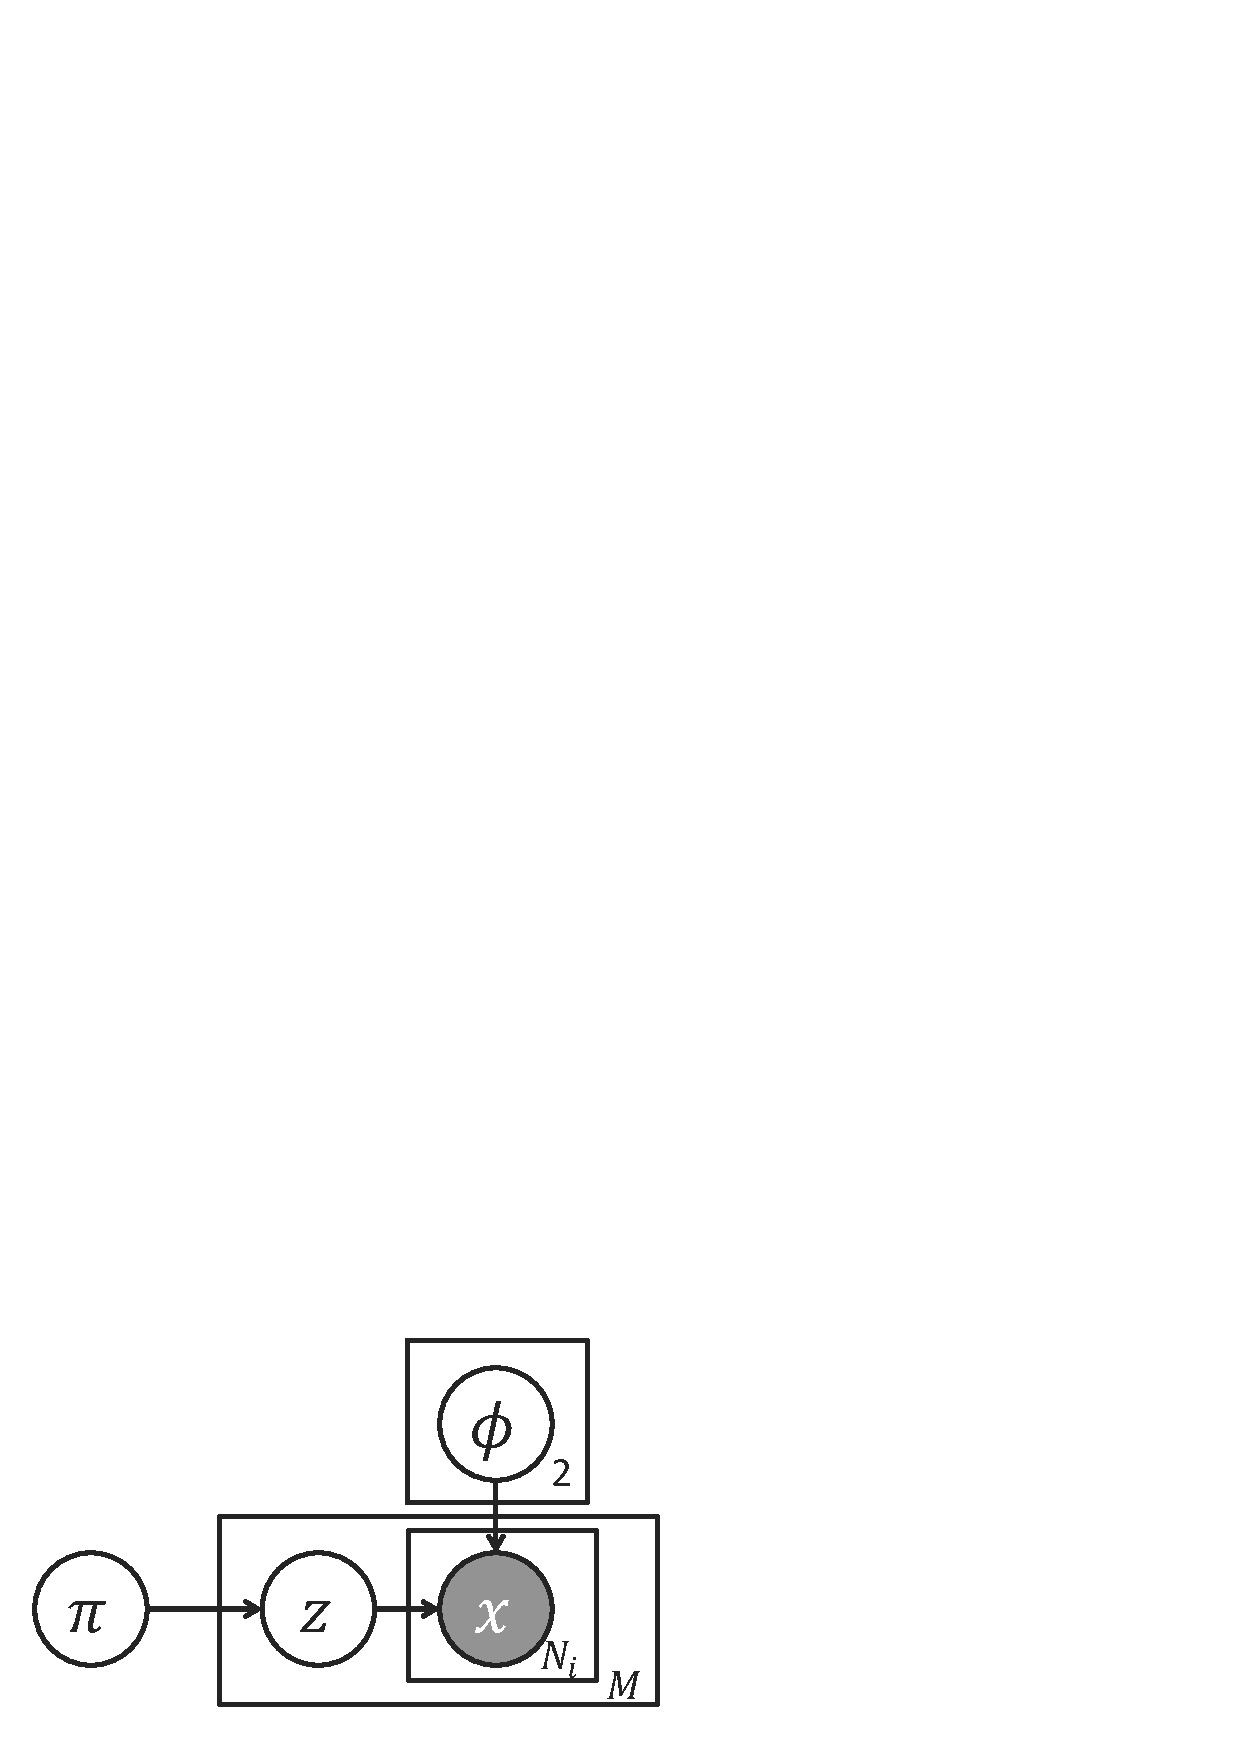
\includegraphics[width=0.25\textwidth]{figs/two_coins_nestedplates}
	\caption{Two-coin Model with Nested Plates}
	\label{fig:two_coins_nestedplates}
\end{figure}

\subsection{Bayesian Network Construction}

\begin{figure}[h]
\centering
\includegraphics[scale=0.4]{figs/two_coins_bn1.eps}
\caption{Bayesian Network Template Constructed from the Two-coin Model}
\label{fig:two_coins_bn1}
\end{figure}

An input InferSpark program is first parsed and separated into two parts: 
the model definition (``{\sf @Model} class TwoCoins'' in 
\figref{fig:two_coins_modeldef}) and
the ordinary scala program (``{\sf object Main}'' in
\figref{fig:two_coins_modeldef}). The model definition is analyzed and
transformed into valid scala classes that define a Bayesian
network constructed from the model definition 
(e.g., \figref{fig:two_coins_bn1}) and the inference/query API.
Note the Bayesian network
constructed at this stage is only a template (different than 
\figref{fig:two_coin_bn}) because some of the information is not available 
until run time (e.g., the outcomes $x$, the number of coin flippings 
and the model parameters $\alpha$ and $\beta$). 
%A snippet of generated two-coin code (with simplified variable names)
%is shown in \figref{fig:two_coins_stage1code}.
%
%\begin{figure}[h]
%\centering
%\begin{lstlisting}
%class TwoCoins(alpha: Double, beta: Double) extends ModelBase {
%	val synval$internal$parent: Array[Int] = /**/
%	var Categorical$13$isObserved: Boolean = _
%	class Categorical$13$Inferface extends RandomVariable {
%		def observe(obs: RDD[Long]) = /* ... */
%		def getResult(): RDD[CategoricalResult] = /* ... */
%	}
%	val x = new Categorical$13$Interface()
%	/* ... */
%}
%\end{lstlisting}
%\caption{Bayesian Network Code}
%\label{fig:two_coins_stage1code}
%\end{figure}
%
%The Bayesian network source code is then compiled with the
%ordinary scala program into bytecode. This bytecode will generate the
%inference code of the VMP algorithm for the model on GraphX in
%the next 4 steps.
%
%The InferSpark model definition is a scala definition with ``@Model''
%annotation. The scala parser first separates the model definition from other
%part of the program (i.e. user program). A Bayesian network is then constructed
%according to dependencies between the random variables in the model definition.
%\figref{fig:lda_bn1} is the Bayesian network constructed from the LDA model
%definition. Some information only available at runtime are missing from the
%Bayesian network, e.g. the number of topics $K$, the observed words $w$, etc.
%At this step, the analyzer also verifies that the model is in the
%exponentail-conjugate family and rejects unsupported model definitions. After
%the construction, the Bayesian network is stored in the compiled program for
%later steps to process.

%\begin{figure}[!h] 
%	\centering 
%	\includegraphics[scale=0.3]{figs/lda_bn1.eps}
%	\caption{Bayesian Network Constructed From the Model Definition}
%	\label{fig:lda_bn1}
%\end{figure}

\subsection{Metadata Collection}

Metadata such as the observed values and the plate sizes missing from the
Bayesian networks are collected at runtime. In the two-coin
model, an instance of the model is created via the constructor invocation (e.g.
``{\sf val m = new TwoCoin(1.0, 1.0)}'' on line 10 of \figref{fig:two_coins_modeldef}). The constructor call provides
the missing constants in the prior distributions of $\pi$ and $\phi$. 
For each random variable defined in the model definition, 
there is an interface field with the
same name in the constructed object. Observed values are provided to InferSpark
by calling the ``{\sf observe}'' (line 11 of \figref{fig:two_coins_modeldef}) 
API on the field. 
There, the user provides an RDD of observed outcomes ``{\sf xdata}'' to InferSpark by calling
``{\sf m.x.observe(xdata)}''. The  {\sf observe} API also triggers 
the calculation of unknown plate sizes. 
In this case, the size of plate surrounding $z$ and $x$ is
automatically calculated by counting the number of elements in the RDD.

%When the user provide the observed random variables such as the words in the
%LDA model, the number of documents and the number of words in each document
%can be inferred from the data. This is different from most libraries in that
%they require the user to explicitly set the numbers or to transform the data
%into a library-specific format. InferSpark also tries to verify that the user
%have provided consistent data. For example, InferSpark will report an error,
%if the user provides data to both the topics $z$ and the words $w$ but they
%have differnt sizes.

\subsection{Code Generation}

\begin{figure}
\centering
	\includegraphics[width=0.35\textwidth]{figs/two_coins_msg.eps}
	\caption{Bayesian Network with Messages for Two-coin Model}
	\label{fig:two_coins_msg}
\end{figure}

When the user calls ``{\sf infer}'' API (line 12 of \figref{fig:two_coins_modeldef}) 
on the model instance, InferSpark
checks whether all the missing metadata are collected. If so, it proceeds to
annotate the Bayesian network with messages used in VMP, resulting in
\figref{fig:two_coins_msg}. The expressions that calculate the messages 
(e.g., $E_{Q_\pi}[\ln \pi]$) depend on not only
the structure of the Bayesian network and whether the vertices are observed or
not, but also practical consideration of efficiency and constraints on
GraphX.  

%The inference algorithm we use is the variational message passing algorithm.
%This step annotates the messages and vertex updates of the algorithm to the
%Bayesian network from previous step and we call the resuling graph as message
%passing graph.
%
%The VMP algorithm is expressed as sending messages of functions of sufficient
%statistics of random variables and updating the sufficient statistics by
%aggregating the messages. The messages are sent in both direction of the edges
%in the Bayesian network. The vertices are updated by aggregating incoming
%messages. For the Dirichlet random variables, the update is simply adding
%together all the messages. The unobserved Categorical random variable $z$ is
%updated by normalizing the sum of the messages. The observed Categorical
%mixtures $w$ have nothing to update but have to compute the new messages to $z$
%and $\phi$ according to the incoming messages.

%\begin{figure}[h]
%	\centering	
%	\includegraphics[scale=0.3]{figs/lda_mpg.eps}
%	\caption{Message Passing Graph of LDA}
%	\label{fig:lda_mpg}
%\end{figure}


%The messages in the VMP algorithm are sent in both directions. The messages
%along the edge only depend on the sender but the messages in the reverse
%direction may also depend on other parents' message.  For example, the message
%along the edge from $z$ to $w$ only depends on the sufficient statistics of
%the Categorical variable $z$, but the reverse one will depend on the
%topic-word distributions' messages. The original VMP algorithm assumes that
%only one vertex may be updated in each step and the messages that the vertex
%depends on are always up-to-date.  However, this poses two challenges when
%implementing it as a distributed message passing algorithm. First, we have to
%relax the assumption of one vertex in each step to increase parallelism
%without violating the correctness of the algorithm. In the LDA example,
%Updating all the random variables at the same time does not guarantee to
%optimize the ELBO but we can update all the topics at the same time because it
%is equivalent to sequentially update each of the topics. Secondly, vertecies
%that have not been updated could send messages that depends on stale messages.
%If updates to the topics $z$ are immediately followed by updates to the
%topic-word distributions $\phi$, the messages from $w$ to $\phi$ will depend
%on the messages sent from $z$ to $w$ prior to the update of $z$ instead of the
%new messages from $z$ to $w$. Therefore, we choose an update schedule that is
%equivalent to sequential updates to ensure the correctness of the algorithm.

%\subsection{MPG Construction Code Generation}
To convert the Bayesian network to a message passing graph on GraphX,
InferSpark needs to construct a VertexRDD and an EdgeRDD. This step generates
the MPG construction code specific to the data.
\figref{fig:two_coins_mpg_constr_code} shows the MPG construction code
generated for the two-coin model. 
The vertices are constructed by the union
of three RDD's, one of which from the data and the others from 
parallelized collections (lines 8 and line 9 in \figref{fig:two_coins_mpg_constr_code}).
The edges are built from the data only. 
A partition strategy specific to the
data is also generated in this step.




\begin{figure}[h]
\begin{lstlisting}
class TwoCoinsPS extends PartitionStrategy {
	override def getPartition /**/
}
def constrMPG() = {
	val v1 = Categorical$13$observedValue.mapPartitions{
		initialize z, x */
	}
	val v2 = sc.parallelize(0 until 2).map{ /* initialize phi */ }
	val v3 = sc.parallelize(0 until 1).map{ /* initialize pi */ }
	val e1 = Categorical$13$observedValue.mapParititons{
		/* initialize edges */
	}
	Graph(v1 ++ v2 ++ v3, e1).partitionBy(new TwoCoinsPS())
}
\end{lstlisting}
\caption{Generated MPG Construction Code}
\label{fig:two_coins_mpg_constr_code}
\end{figure}


%Constructing the
%message passing graph of the Bayesian network is not trivial because different
%types of random variables have different initialization methods and different
%data sources. The initialization of the outcomes $x$ in the two-coin model is
%fixing its distribution to a point categorical distribution at the observed
%outcome and randomly initialize the incoming messages while the initialization
%of the choice of coins $z$ is to randomly initialize the parameters of its
%approximate marginal posterior distribution. The data source of $x$ is the
%observed outcomes while $z$ does not have data source. The initialization of
%EdgeRDD is also nontrivial because the links between different random
%variables have different structures. Inferspark finds a transformation plan
%for the MPG construction. A possible plan for the two-coin model is shown in
%\figref{fig:two_coins_mpg_construction_plan}.
%
%\begin{figure}[h]
%	\centering
%	\includegraphics[width=0.45\textwidth]{figs/two_coins_mpg_construction_plan.eps}
%	\caption{MPG Construction Plan of Two-Coin Model}
%		\label{fig:two_coins_mpg_construction_plan}
%\end{figure}

%In a typical GraphX application, the property graph has homogeneous vertex
%properties and edge properties. In the shortest distance application, the
%vertex properties are shortest distance from the origin and edges properties
%are weights. The EM algorithm implementation for LDA in Mllib, which only
%computes the Maximum A Posterior rather than the full posterior, uses the
%vertex properties as topic counts and edge propertices as word counts. However,
%the message passing graph of the VMP algorithm generally have heterogeneous
%vertex properties and edge properties. In the LDA case, we have three types of
%vertecies: observed categorical mixture, unobserved categorical variable and
%unobserved dirichlet variable. The observed categorical mixture needs to store
%the messages from parents and the observed value while the other two types need
%to store the sufficient statistics. The edges also have differnt structures.
%There's one-to-one correspondence between $z$ and $w$ while $w$ are fully
%connected to $\phi$. Therefore, the compiler need to create an unrolling plan
%so that the graph is correctly initialized. In the LDA case, a possible plan is
%to first map from the observations of x to create vertecies for $\theta$, $z$
%and $x$ and use a parallelized range to create verticies for $\phi$. Another
%possibility is to separately initialize each set of variables.  We try to
%minimize the overhead of union by merging the initialization of variables as
%much as possible.

In addition to generating code to build the large message passing graph,
the codegen module also generates code for VMP iterative inference. 
InferSpark, which
distributes the computation, needs to create a schedule of parallel updates
that is equivalent to the original VMP algorithm, which only updates one vertex
in each iteration.  Different instances of the same random variables can be
updated at the same time. An example update schedule for the two-coins model is
($\pi$ and $\phi$) $\rightarrow$ $x$ $\rightarrow$ $z$ $\rightarrow$ $x$. VMP inference code that enforces the update
schedule is then generated. % \ERIC{how to derive this indeed?}

\subsection{Getting the Results}
%InferSpark finally compiles the VMP algorithm into a separate GraphX
%program and submit it to the Spark master. The user can specify how many
%iterations to run. 
The inference results can be queried through the ``{\sf getResult}''
API on fields in the model instance that retrieves a VertexRDD of approximate
marginal posterior distribution of the corresponding random variable. For
example, in Line 13 of \figref{fig:two_coins_modeldef}, ``{\sf m.phi.getResult()}'' 
returns a VertexRDD of two Dirichlet distributions. 
The user can also call ``{\sf lowerBound}'' 
on the model instance to get the evidence lower bound (ELBO) of the result, 
which is higher when the KL divergence between the approximate posterior 
distribution and the true posterior is smaller. 

\begin{figure}[h]
\centering
\begin{lstlisting}
var lastL: Double = 0
m.infer(20, { m =>
	if ((m.roundNo > 1) || 
		(Math.abs(m.lowerBound - lastL) < 
		   Math.abs(0.001 * lastL))) {
		false
	} else {
		lastL = m.lowerBound
		true	
	}
})
\end{lstlisting}
\caption{Using Callback function in ``infer'' API}
\label{fig:two_coins_callback}
\end{figure}

The user can also provide a callback function that will be called after
initialization and each iteration. In the function, the user can write
progress reporting code based on the inference result so far. 
For example, this function may return {\em false} whenever
the ELBO improvement is smaller than a threshold 
(see \figref{fig:two_coins_callback}) indicating the result is good enough 
and the inference should be terminated. 

%With all the information collected and calculated in previous steps,
%implementation of the inference algorithm as a GraphX program is generated,
%compiled and then executed. User can retrieve the posterior distributions as
%VertexRDDs through API calls.


\section{Demostratation Plan}
\label{sec:demoplan}

%For demostratation purpose, we have built two systems, one streams real-time TV videos and 
%the other simulates the TV watching using the same weekly schedule. The latter, which is called
%``PredicTV (survey)'', is necessary because
%capturing user behavior on real TV takes a lot of time, and a simulator significantly speeds up
%our evaluation. A total of 81 channels are included in the systems.
%For each channel, we provide two beams of signals and the schedule within the whole week.
%Our service is available in pubic network. And when you watch shows in our system, 
%we will give you some recommendations.
%We also built an survey system. In the real system, we have to wait a long period of time until the user gives us reply.
%In experiment, we cannot wait so much long time. So we come up with an idea to build a survey system which can quickly collect user's viewing behavior.
%The survey system uses the same schedula data and try to simulate the true TV in a simple but effecitve manner.
%More or less, there are some information lost in simulation. But our survey system can provide enough information to caputre user's preference.
%Both systems use the same recommendation algorithms, 
%and behave the same way given the same viewing sequence.
%if a user watches program on one system and we put the viewing history to another, 
%the recommendation result will be same.

\begin{figure}[h]
\begin{center}
\epsfig{file=TV1TV2.eps,width=\columnwidth}
\caption{Snapshots of Demo: (a) PredicTV (realtime) (b) PredicTV (survey)}
\label{fig:TV1TV2}
\end{center}
\end{figure}

Figure \label{fig:TV1TV2} gives a snapshot of our system and 
they are available online \cite{tv-url}. Next we describe
three scenarios that help illustrate the features of the system. Then
we present the setup of the demo. 

%We will present our system thoroughly in our demo.
%First, we use three Scenarios to reveal our recommendation system's features.
%Next, we will focus on how we demostrate our system.

\subsection{Scenarios}

\begin{figure}[h]
\begin{center}
\epsfig{file=final.eps,width=\columnwidth}
\caption{Scenario 1: Latent Relations}
\label{fig:scenario1} 
\end{center}
\end{figure}

In scenario 1, we show how the system discover latent relations among
TV programs (Figure \ref{fig:scenario1}).
User first watches ``You Are The One'', 
a popular match-making reality
show on JSTV. The system recommends ``If You Are The One'', a movie which
shares the same Chinese name and also features a romantic story 
about match-making. After user watches ``If You Are the One'', 
the system recommends ``Be There Or Be Square'', another romantic movie 
directed by renown director Feng Xiaogang, who happened to direct 
``If You Are The One'' as well. Now, when the user again follows the
recommendation to watch ``Be There Or Be Square'', the system further
suggests ``Good Luck''. It turns out that both of these movies starred
Ge You, a popular actor in China.

%Both ``If You Are The One'' and ``My Man Can'' are reality shows hosted by the
%same is a show which has the same host and broadcasts on the same channel with "My Man Can".
%Meanwhile, "If You Are The One" is also a movie directed by Feng Xiaogang. 
%A famous chinese actor Ge You plays a role in this film.
%"Be There or Be Square" is aothner film directed by XiaoGang Feng. You Ge also plays a role in it. So our system recommends this moive to user.
%After the user watches "If You Are The One" and "Be There or Be Square",
%the system recommends "Good Luck" which again involves XiaoGang Feng and You Ge but isn't very famous to public.
%

Scenario 2 illustrates how the system adapts to the changes of user watching
behavior. When user watches 
``Scientific Career: Scientist's Life Experience'' 
and ``Exploration \& Discovery: Remove the Veil'', two science-related
program, the system suggest a reality show ``I'm An Adventure King''. 
Now suppose the user changes his interest to news programming, and 
watches ``30 Minutes in News'', the system captures this change
and recommends ``News Studio.'' The rate at which the system adapts to
such changes is determined by a decay parameter.

%We can see clearly the system captures user's preference changing. Originally, the user prefers scientific and technical program and adventure program.
%Our system captures this perference and then gives a adventure show. 
%Then user changes his interest. He begins to watch news program. 
%Our system do follow the interest change.
%After the user watch a news show, our system recommends news program 
%instead of advanture program. Actually, 
%how fast the system react to user's interest change is a
%configurable parameter in our system. The higher the value, 
%the slower the reaction.

In Scenario 3, multiple users share a TV set in a household
and watches TV at different times of the day. Suppose the grandma watches
``Beautiful Sunset'', a program for senior citizens, at 8:30 AM whereas
the grandson watches ``Cartoon First!'' from 4:15 PM to 7 PM.
The system would detect such regularity and suggest health-related programs
in the morning, while recommends ``Big Wind Mill'', an education program for
kids, in the late afternoon.

%When user watches "First Time:Information wake up everyday" from 8:00 a.m. to 9:00 a.m. on Monday and Tuesday morning,
%our system recommends programs which are all in the morning such as
%"Good Morning, HaHa(7:00)" and "Morning New Horizon(7:00)".
%
%It's the result from the recommendation results partitioning feature.
%We assume user watches program in a particular period of time, such as, children usually watch program on evening and workers usually watch program on morning and evening.
%Thus we partition the recommendation results into different time slot.
%If we detect the user usually watches shows on morning, then we give them recommendations in the morning slot instead of the whole day.

\subsection{Demo Setup}

%First, we will use a poster to give an overview of the system, including the motivation and major issues 
%addressed in the system. We will introduce the architecture and the main features of the system.
%
Before the demo, we will download and analyze the schedule for all 
81 channels for the week in which the conference takes place. 
We will identify the 3 aforementioned scenarios in this 
schedule and prepare concrete story lines. 
We will perform information extraction before hand for the programs in
that schedule and establish program models. 
During the actual demo, we will let the visitor first experience 
PredicTV(Real-time) by watching a few shows and observing the recommendation 
results. We then instruct her to repeat the same viewing sequence on
PredicTV(Survey). She will notice that the recommendations on the
survey is the same and hence understand the equivalence of the two systems.
From that point, we will guide her through the 3 scenarios on the survey
system.
%
%Next, we show that survey system and real video stream system have the same recommendation algorithm.
%We will use 3-4 different examples. After the examples, users can watch some shows by 
%their own interests on both system. They will see the same recommendation result.
%
%Then, the system will be open for all users. They can try on their own interests and get corresponding recommendation results.
%We will explain our system and new features while they play with our system.
%
%Finally, we will give a brief conclusion about TV recommendation, including what the status of current research on this topic is and what difficluties we are facing
%and what we will do in next step.
%
%Please note that this is an ongoing project. Visitors should expect the system to change. We are developing new algorithm and extracting more information about TV program.

%!TEX root = paper.tex

\section{Related Work}
\label{sec:related}

MLlib, Mahout \cite{mahout}, and MADLib \cite{madlib} are machine learning \emph{libraries} on top of distributed computing platforms and relational engines.
All of them provide many standard machine learning models such as LDA and SVM.
However, when a domain user, say, a machine learning researcher, 
is devising and testing her customized models with her big data, 
those libraries cannot help.

MATLAB and R have been the most popular systems for implementing inference algorithms.
They, however, can hardly scale up when faced with increasing amount of data
because they mostly work on a single machine and thus cannot easily scale out.
It is possible to first transform a large dataset into a smaller one
using MapReduce or Spark and then load the data to MATLAB or R to perform inference %on the smaller ones in
in some scenarios. But this approach involves multiple systems, which is hard to
develop code for and inefficient because of the data movement.
SystemML \cite{systemml} provides a similar interface for implementing inference
algorithms and transforms them to Hadoop MapReduce. It can scale out to large
clusters but coding on such a system still requires extensive knowledge in
statistical inference for end-user. 

In contrast to the systems above, MLBase \cite{mlbase} targets end-users who are not
machine learning experts. It exposes a declarative language interface and
provides a cost-based optimizer that selects the best algorithm and
parameters. It also provides MLI \cite{mli}, a set of APIs for customizing algorithms on
Spark. However, MLBase mainly supports frequentist approach, such as SVM,
and logistic regression. It does not deal with general Bayesian inference. 

There are a number of probabilistic programming frameworks other than
Infer.NET \cite{InferNET14}.  For example, Church \cite{GMR+08} is a
probabilistic programming language based on the functional programming
language Scheme.  Church programs are interpreted rather than compiled.
Random draws from a basic distribution and queries about the execution trace
are two additional type of expressions. A Church expression defines a
generative model. Queries of a Church expression can be conditioned on any
valid Church expressions. Nested queries and recursive functions are also
supported by Church. Church supports stochastic-memoizer which can be used to
express nonparametric models.  Despite the expressive power of Church, it
cannot scale for large dataset and models.  Figaro is a probabilistic
programming language implemented as a library in Scala \cite{Figaro}.  It is
similar to Infer.NET in the way of defining models and performing inferences
but put more emphasis to object-orientation. Models are defined by composing
instances of Model classes defined in the Figaro library.  Infer.NET is a
probabilistic programming framework in C\# for Bayesian Inference. A rich set
of variables are available for model definition. Models are converted to a
factor graph on which efficient built-in inference algorithms can be applied.
Infer.NET is the best optimized probabilistic programming frameworks so far.
Unfortunately, all existing probabilistic programming frameworks including
Infer.NET cannot scale out on to a distributed platform.

To the best of our knowledge, InferSpark is the only framework that can
efficiently carry out large-scale Bayesian inference through probabilistic
programming on a distributed in-memory computing platform. It targets
end-users who are not expert in Bayesian inference or distributed computing.
The inference implementation can scale out to a large cluster and scale up to
large datasets.

%
%Our proposed probabilistic programming language is also an extension to the existing language Scala, but differs from the way that Infer .NET and Figaro define models that we add additional language constructs to Scala rather than implement a library. It typically enables a cleaner syntax. 







%\item Other inference algorithms for Bayesian Networks.



\cut{%%%%%%%%%%%%%%
The Apache Hadoop library \cite{hadoop} is a distributed data storage and processing framework. Its distributed file system HDFS support the storage of large data. MapReduce is the programming model for distributed parallel processing of the large data. It is composed of two key operations map and reduce. Map operation transforms and filters the data on different nodes in parallel while reduce operations combines the results from map operation to produce results grouped by keys. In our proposal of PP, data can be distribted on a HDFS.

Spark is another distributed data processing framework that provides MapReduce operations. It differs from Hadoop in that it does not write the intermediate results to temporary storage. Instead, it caches the results in memory as resilient distributed dataset \cite{Zaharia:2012:RDD:2228298.2228301}. It can greatly speed up the processing. 

The Spark built-in machine learning library MLlib \cite{mllib} provides a variety of standard statistical inference algorithms including classification, regression, clustering, collaborative filtering and dimensionality reduction. The algorithms leverage the Spark infrastructure so that large-scale data can be processed efficiently. The algorithms are applicable when the standard models fit the data well. Users have to directly develop their own algorithms using Spark or GraphX API when a customized model has to be used. Our integration of PP with Spark can greatly reduce the amount of work to implement a new model.

GraphX \cite{Xin:2013:GRD:2484425.2484427} is Spark's built-in graph parallel computation API. User can view graphs as normal RDDs of vertices and edges and perform normal map reduce operations on them or perform graph operations like compute subgraph, reversing edges, join vertices. The Pregel operator in GraphX is used to express iterative algorithms. In each step, vertices aggregates messages along the inbound edges from previous step, compute its new value and sends messages along outbound edges in parallel. It terminates when no message is sent during a step. Our PP will be built on GraphX since it is natural to represent the factor graph in GraphX and leverage the parallel graph computing to implement message-passing style inference algorithms.

\KZ{Reduce the discussion of the following PP languages a bit. Focus on
their big-data handling capabilities, or the lack of which.}

Many recent probabilistic programming languages are implemented by extending existing conventional programming languages such as Scheme, C\#, Scala and etc.
We examine three probabilistic programming languages Church \cite{GMR+08}, Infer .NET \cite{InferNET14} and Figaro \cite{pfeffer2009figaro}.

Church is a probabilistic programming language based on the functional programming language Scheme. Random draws from a basic distribution and queries about the execution trace are two additional type of expressions. A church expression defines a generative model. Queries of a church expression can be conditioned on any valid church expressions. Nested queries and recursive functions are also supported by Church. Church supports stochastic-memoizer which can be used to express nonparametric models. Thus a wide range of probabilistic models can be concisely expressed in Church. Inference in Church is implemented by rejection sampling and Metropolis-Hastings sampling algorithms. Despite the expressive power of Church, it cannot scale up to large dataset and models. 

Our approach differs from Church in that our program is compiled rather than interpreted. Compiled program is usually more efficient than interpreted ones. We can also leverage the distributed parallel processing to scale up to large dataset and models.

Infer .NET is a probabilistic programming framework in C\# for Bayesian Inference. A rich set of variables are available for model definition. Models are converted to a factor graph on which efficient built-in inference algorithms can be applied. The algorithms include expectation propagation, variational message passing, block Gibbs sampling. Infer .NET addresses the scalability by shared variables, as discussed in Section \ref{sec:intro}.
%% ?? not sure about how the shared variable is implemented

Figaro is a probabilistic programming language implemented as a library in Scala. It is similar to Infer .NET in the way of defining models and performing inferences but put more emphasis to object-orientation. Models are defined by composing instances of Model classes defined in the Figaro library.

Our proposed probabilistic programming language is also an extension to the existing language Scala, but differs from the way that Infer .NET and Figaro define models that we add additional language constructs to Scala rather than implement a library. It typically enables a cleaner syntax. 

}%%%%%%%%%%%%%%%%

%%!TEX root = paper.tex
\section{Implementation}
\label{sec:implementation}
The main jobs of InferSpark are Bayesian network construction and  code generation (\figref{fig:workflow}).
Bayesian network construction first extracts Bayesian network template from the model definition and transforms it into a
Scala class with inference and query APIs at compile time. 
%The generated class
%is compiled with normal scala part of the program 
%Then, code generation takes those as inputs and generates a Spark program which 
%including the messaging passing graph and VMP inference code. Afterwards, the generated program is executed on Spark.
Then, code generation takes those as inputs and generates a Spark program
that can generate the messaging passing graph with VMP on top.
Afterwards, the generated program would be executed on Spark.

We use the code generation approach because it enables a more flexible API
than a library. For a library, there are fixed number of APIs for user to
provide data, while InferSpark can dynamically generate custom-made APIs 
according to the structure of the Bayesian network. 
Another reason for using code generation is
that compiled programs are always more efficient than interpreted programs.

%The code generation to implement InferSpark. 
%Stage 1 constructs
%a and submitted to Spark.  
%Stage 2 performs metadata collection using Spark and generate MPG 
%construction and VMP inference code based on the meta data at run time.


%\subsection{Stage 1 Code Generation}
\subsection{Bayesian Network Construction}\label{bnc}

In this offline compilation stage, the model definition is first transformed into a Bayesian network.
We use the macro annotation, a compile-time meta programming facility of
Scala.  It is currently supported via the macroparadise plugin. After the
parser phase, the class annotated with ``{\sf @Model}'' annotation is passed from the
compiler to its transform method. InferSpark treats the class passed to it as
model definition and transforms it into a Bayesian network.

\begin{figure}[!h]
\scriptsize
	\begin{tabular}{lrl}
		ModelDef		& ::= & `@Model' `class' id \\
					&     &`(' ClassParamsOpt `)' `\{' Stmts `\}' \\
		ClassParamsOpt	& ::= & `' /* Empty */ \\
						&	| &	ClassParams \\
		ClassParams		& ::= & ClassParam  [`,' ClassParams] \\
		ClassParam		& ::= & id `:' Type \\
		Type			& ::= & `Long' | `Double' \\
		Stmts			& ::= & Stmt [[semi] Stmts]\\
		Stmt			& ::= & `val' id = Expr \\
		Expr			& ::= & `\{' [Stmts [semi]] Expr `\}' \\
						&	| & DExpr	\\
						&   | & RVExpr \\
						&	| & PlateExpr \\
						&	| & Expr `.' `map' `(' id => Expr `)'\\
		DExpr			& ::= & Literal	\\
						&   | & id \\
						&   | & DExpr (`+' | `-' | `*' | `/') DExpr \\
						&   | & (`+' | `-') DExpr	\\
		RVExpr			& ::= & `Dirichlet' `(' DExpr `,' DExpr `)' \\
						&   | & `Beta' `(' DExpr `)' \\
						&   | & `Categorical' `(' Expr `)' \\
						&   | & RVExpr RVArgList	\\
						&   | & id	\\
		RVArgList		& ::= & `(' RVExpr `)' [ RVArgList ] \\
		PlateExpr		& ::= & DExpr `until' DExpr	\\ 
						&   | & DExpr `to' DExpr	\\
						&	| & `?' \\
						&	| & id
	\end{tabular}
\caption{InferSpark Model Definition Syntax}
\label{fig:inferspark_syntax}
\end{figure}

\figref{fig:inferspark_syntax} shows the syntax of InferSpark model
definition. The expressions in a model definition is divided into 3
categories: deterministic expressions (DExpr), random variable expressions
(RVExpr) and plate expressions. The deterministic expressions include
literals, class parameters and their arithemetic operations. The random
variable expressions define random variables or plates of random variables.
The plate expressions define plate of known size or unknown size. The random
variables defined by an expression can be binded to an identifier by the value
definition. It is also possible for a random variable to be binded to multiple
or no identifiers. To uniquely represent the random variables, we assign
internal names to them instead of using the identifiers.

\begin{figure}[ht]
\centering
	\includegraphics[width=0.6\columnwidth]{figs/two_coins_internal_bn1.eps}
	\caption{Internal Rep. of Bayesian Network}
	\label{fig:two_coins_internal_bn1}
\end{figure}

Internally, InferSpark represents a Bayesian network in a tree form, where the
leaf nodes are random variables and the non-leaf nodes are plates. The edges
in the tree represent the nesting relation between plates or between a plate
and random variables. The conditional dependencies in the Bayesian network are
stored in each node.  The root of the tree is a predefined plate TOPLEVEL with
size 1.  \figref{fig:two_coins_internal_bn1} is the internal representation of
the two-coin model in \figref{fig:two_coins_bn1}, where
$r_1$, $r_2$, $r_3$, $r_4$, correspond to $\pi$, $\phi$, $z$, $x$, respectively. 
Plate 1 and Plate 2 correponds to the plates defined on lines 3--5 in
\figref{fig:two_coins_modeldef}. 

If a plate is nested within another plate,
the inner plate is repeated multiple times, in which case,
the size attribute of the plate node will be computed by summing the size of each
repeated inner plate. We call the size attribute in the tree {\em flattened size}
of a plate. For example, in \figref{fig:two_coins_nestedplates}, the flattened
size of the innermost plate around $x$ is $\sum_i N_i$.

%\begin{figure*}[!h]
%\centering
%\scriptsize
%	\begin{tabular}{|p{0.45\textwidth}|p{0.45\textwidth}|}
%		\hline
%%		ModelDef ::= @Model class id (ClassParamsOpt) \{ Stmts \} & 
%%		\begin{tabular}{l}
%%			env = {}; \\
%%			curPlate = TOPLEVEL;\\
%%			transform(ClassParamsOpt, curPlate, env); \\
%%			transform(Stmts, curPlate, env); \\
%%			genCode(TOPLEVEL, env);
%%		\end{tabular}\\\hline
%%
%%		ClassParams ::= ClassParam [, ClassParams] & 
%%		\begin{tabular}{l}
%%			transform(ClassParam, curPlate, env);\\
%%			transform(ClassParams, curPlate, env);
%%		\end{tabular} \\\hline
%%
%		ClassParam ::= id ':' Type &
%		\begin{tabular}{l}
%			env.push(id, ClassParam(Type))
%		\end{tabular} \\\hline
%%
%%		Stmts ::= Stmt [[semi Stmts]] &
%%		\begin{tabular}{l}
%%			transform(Stmt, curPlate, env);\\
%%			transform(Stmts, curPlate, env);
%%		\end{tabular} \\\hline
%%
%%		Stmt ::= val id = Expr &
%%		\begin{tabular}{l}
%%			r = eval(Expr, curPlate, env); \\
%%			env.put(id, r);
%%		\end{tabular} \\\hline
%%
%%		Expr ::= \{ [Stmts [semi]] Expr \} &
%%		\begin{tabular}{l}
%%			transform(Stmts, curPlate, env);	\\
%%			return eval(Expr, curPlate, env);	
%%		\end{tabular} \\\hline
%%
%		Expr ::= DExpr &
%		\begin{tabular}{l}
%			return DExpr;
%		\end{tabular} \\\hline
%%
%%		Expr ::= RVExpr &
%%		\begin{tabular}{l}
%%			return eval(RVExpr, curPlate, env);
%%		\end{tabular} \\\hline
%%
%%		RVExpr ::= Dirichlet(DExpr1, DExpr2) &
%%		\begin{tabular}{l}
%%			alpha = eval(DExpr1, curPlate, env);	\\
%%			dim = eval(DExpr2, curPlate, env);	\\
%%			if (alpha.type != Double || dim.tpe != Long) error;	\\
%%			r = Dirichlet(alpha, dim);	\\
%%			curPlate.addChild(Dirichlet(alpha, dim));	\\
%%			return d;
%%		\end{tabular} \\\hline
%%
%%		RVExpr ::= Beta(DExpr) &
%%		\begin{tabular}{l}
%%			alpha = eval(DExpr, curPlate, env);	\\
%%			if (alpha.type != Double) error; \\
%%			r = Dirichlet(alpha, 2); \\
%%			curPlate.addChild(r); \\
%%			return r;
%%		\end{tabular} \\\hline
%%
%		RVExpr ::= Categorical(Expr) &
%		\begin{tabular}{l}
%			p = eval(Expr, curPlate, env); \\
%			if (p.type != DoubleVector) error;\\
%			if (p.isRV \&\& p is not Dirichlet) error;\\
%			r = Categorical(p); \\
%			curPlate.addChild(r); \\
%			return r;
%		\end{tabular} \\\hline
%
%		RVExpr ::= RVExpr RVArgList &
%		\begin{tabular}{l}
%			(r, plate) = eval(RVExpr, curPlate, env);\\
%			argList = eval(RVArgList, curPlate, env); \\
%			if (argList.length != r.depth - plate.depth) error;\\
%			if (argList.find(!conjugate to r || type is not Long)) error;\\
%			return Mixture(r, plate, argList);
%		\end{tabular} \\\hline
%%
%%		RVExpr ::= id &
%%		\begin{tabular}{l}
%%			return env.get(id);
%%		\end{tabular} \\\hline
%%
%%		PlateExpr ::= DExpr1 until DExpr2 &
%%		\begin{tabular}{l}
%%			low = eval(DExpr1, curPlate, env);\\
%%			high = eval(DExpr2, curPlate, env); \\
%%			p = Plate(ExclusiveRange(low, high)); \\
%%			curPlate.addChild(p);
%%			return p;
%%		\end{tabular} \\\hline
%%
%%		PlateExpr ::= DExpr1 to DExpr2 &
%%		\begin{tabular}{l}
%%			low = eval(DExpr1, curPlate, env);\\
%%			high = eval(DExpr2, curPlate, env); \\
%%			p = Plate(InclusiveRange(low, high)); \\
%%			curPlate.addChild(p);
%%			return p;
%%		\end{tabular} \\\hline
%%
%		PlateExpr ::= ? &
%		\begin{tabular}{l}
%			p = Plate(UnknownRange); \\
%			curPlate.addChild(p);
%			return p;
%		\end{tabular} \\\hline
%
%		Expr ::= Expr1.map(id => Expr2) &
%		\begin{tabular}{l}
%			left = eval(Expr1, curPlate, env);\\
%			if (left is plate) \{\\
%				r = eval(Expr2, left, env);\\
%				return (r, left); \\
%			\} else if (left = (r1, plate)) \{ \\
%				env.put(id, (r1, plate(r1)));\\
%				r2 = eval(Expr2, plate, env);\\
%				env.pop(id);\\
%				return (r2, plate);\\
%			\} else error;
%		\end{tabular}\\\hline
%
%	\end{tabular}
%	\caption{Transformation Rules}
%	\label{fig:transformation_rules}
%\end{figure*}

InferSpark recursively descends on the abstract syntax tree (AST) of the model definition to construct
the Bayesian network.   In the
model definition, InferSpark follows the normal lexical scoping rules.
%\figref{fig:transformation_rules} shows part of the transformation rules of each
%syntax. ``transform(ast, curPlate, env)'' transforms non-expression parts while
%``eval(ast, curPlate, env)'' transforms expression and result the evaluation result.
InferSpark evaluates the expressions to one of the following three results
\begin{itemize}
	\item a node in the tree
	\item a pair $(r, \textrm{plate})$ where $r$ is a random variable node
		and plate is a plate node among its ancestors, which represents all
		the random variables in the plate
	\item a determinstic expression that will be evaluated at run time
\end{itemize}
%When defining the random variables, InferSpark also checkes the conjugacy
%constraints of the Bayesian network.

At this point, apart from constructing the Bayesian network representation, 
InferSpark also generates the code for metadata collection, a module used in 
stage 2. For each random variable name bindings, a singleton interface object 
is also created in the resulting class. 
The interface object provides ``{\sf observe}'' and ``{\sf getResult}'' API for later use.

%Value definitions ``val'' id ``='' Expr has two functionalities in InferSpark.
%First, it binds the result of the evaluation result of an expression to an
%identifier. Secondly, it declares an interface singleton
%object for the random variable that the right hand side evaluates to.
%For value definitions that inside a plate, the singleton object
%is nested inside the outer object at definition site. For example, 
%
%\begin{figure}[h]
%\begin{lstlisting}[numbers=none]
%	val trial = ?.map{_ =>
%		val z = Categorical(pi)
%		val x = ?.map{_ => Categorical(phi(z))
%	}
%\end{lstlisting}
%\caption{Path Of Interface}
%\label{sec:path}
%\end{figure}
%defines multiple trials in which we first choose a coin and then flip it for
%multiple times. The interface singleton generated is ``trial.z'' ``trial.x''.
%To implement this feature, Inferspark calculates the path, a list of
%identifiers in the chain of value definitions. For ``z'' and ``x'', the path
%are [``trial'', ``x''] and [``trial'', ``z'], respectively.
%
%In Inferspark, the Bayesian network is represented as a tree.
%\figref{fig:two_coins_internal_bn1} is the internal representation of the
%Bayesian network of two-coin model, where $r_1$, $r_2$, $r_3$, $r_4$,
%correspond to pi, phi, z, x, respectively. The non-left nodes of the tree is
%always plates while the leaf nodes are either random variable or empty plate.
%The root is a predefined plate with constant size 1 called TOPLEVEL. The depth
%of TOPLEVEL is 0. Child node has depth one larger than parent (e.g. $r_1$,
%plate 1 and 2 are of depth 1, the others are of depth 2).
%
%An expression evaluates to one of the following three:
%\begin{itemize}
%	\item a node in the tree
%	\item a pair $(r, \textrm{plate})$ where $r$ is a random variable node
%		and plate is a plate node among its ancestors
%	\item a determinstic expression that will be evaluated at run time
%\end{itemize}
%and is divided into 3 categories: deterministic expression, random variable
%expression and plate expression.
%
%Deterministic expression can be literals of Long and Double, class parameters
%or arithmetic operations on deterministic expressions. It evaluates to itself.
%
%Plate expression includes exclusive range (e.g. ``0 until 1''), inclusive
%range (e.g. ``0 to 1'') and unknown range ``?''. Plate expressions always
%create new plates. Plate expression evaluates to the node of the new plate.
%
%Random variable expression includes primitive random distributions and
%mixture. The primitive random distributions we currently support are Beta,
%Dirichlet and categorical distribution. The parameters of the distributions
%can be a deterministic value or a random variable node. The mixture expression
%is of form ``id(id1)(id2)...(idn)'', where id evaluates to a pair $(r,
%\textrm{plate})$ where the depth of plate is $n$ smaller than that of $r$.
%`id1'' to ``idn'' evaluates to random variable nodes, which selects the
%corresponding component. We have an restriction that ``id1'', ... ``idn'' are
%independent, which we may remove in the future work.
%
%``map'' call can be applied to a plate node plate or a pair $(r,
%\textrm{plate})$. When it is applied to a plate node, the formal parameter of
%the anonymous function argument is ignored. When it is applied to a pair $(r,
%\textrm{plate})$, the formal parameter of the anonymous function is binded to
%the $r$ if $r$'s parent in the tree is plate, or another pair ($r$, plate')
%where plate' is child of plate and is ancestor of $r$. For both cases, the
%body of the anonymous function can be a sequence of value definitions followed
%by an expression. The plate or random variables defined inside the body is put
%in plate. If the body expression evaluates to a random variable node $r'$ or a
%pair $(r', \textrm{plate}')$, the ``map'' evaluates to ($r$, plate).  
%
%For example, line 4 first defines plate 2 with unknown size in the TOPLEVEL.
%Then it applies ``map'' to plate 2. Inside the anonymous function, a
%Categorical variable $r_3$ is defined and put in plate 2. The ``map''
%evaluates to a pair $(r_3, \textrm{plate 2})$, which is binded to identifier
%z. On line 5, the outermost identifier z evaluates to a pair $(r_3,
%\textrm{plate 2})$.  When ``map'' is applied to it, the formal parameter ``z''
%is binded to $r_3$. The anonymous function body defines a categorical mixture
%$r_4$ and``map'' evaluates to $(r_4, \textrm{plate 2})$. Finally, $(r_4,
%\textrm{plate 2})$ is binded to the identifier x.
%
%After the construction of the Bayesian network, Inferspark generates code that
%implements the metadata collection (e.g. ``observe'') and parts of the second
%stage compilation. These parts depends on the structure of the Bayesian
%network thus must be generated. For example, x in the two-coin model is a
%Categorical random variable inside a plate size so the observed data type is
%``RDD[Long]''. ``trial.x'' in the \figref{fig:path} has two nested plates
%around it, so the observed data type is ``RDD[Array[Long]]''. Parts that do
%not depend on the structures are put into the precompiled runtime libarary of
%Inferspark. The implementation of both parts are discussed in next subsection.

\subsection{Code Generation}

Code generation happens at run time. It is divided into 4 steps: metadata
collection, message annotation, MPG construction code generation and inference
execution code generation.

Metadata collection aims to collect the values of the model parameters,
check whether random variables are observed or not, the flattened sizes of the plates.
These metadata can help to 
assign VertexID to the vertices on the message passing graph.  
%If a plate is the innermost plate that a random variable is in, the flat size of
%the plate is defined as the number of this random variable. For example, the
%flat size of plate 2 in \figref{fig:two_coins_internal_bn1} is the number of
%outcomes $x$ or the number of the random variable $z$.  
After the flattened sizes of plates are calculated, we can assign VertexIDs to the
vertices that will be constructed in the message passing graph. Each random
variable will be instantiated into a number of vertices on the MPG where the
number equals to the flattened size of its innermost plate. The vertices
of the same random variable are assigned consecutive IDs. For example, $x$ may
be assigned ID from $0$ to $N-1$. The intervals of IDs of random variables in
the same plate are also consecutive. A possible ID assignment to $z$ is $N$ to
$2N - 1$. Using this ID assignment, we can easily i) determine which random
variable the vertex is from only by determining which interval the ID lies
in; ii) find the ID of the corresponding random variable in the same plate by
substracting or adding multiples of the flattened plate size (e.g. if $x_i$' ID is
$a$ then $z_i$'s ID is $a + N$).

Message annotation aims to annotate the Bayesian Network Template from the previous stage (Section \ref{bnc})
with messages
to be used in VMP algorithm.  The annotated messages are stored in the form of
AST and will be incorporated into the the generated code, output of this stage. 
The rules of the messages to annotate are predefined according to the
derivation of the VMP algorithm.
%The messages between different types of random variables without mixture can
%be created by looking up in a table. For a mixture variable, the message from
%it is composed from basic messages in the table. 
%\KZ{Where is the table, what
%is it like?}
%
%We also need to generate two additional functions for each random variable: a
%message merge function and a vertex update function. 
%\KZ{Don't understand:
%The messages are first
%sent to the vertices to update and merged on the fly, then joined with the
%original vertices to apply the update.}  
After the messages are generated, we
generate for each type of random variable a class with the routines for
calculating the messages and updating the vertex. 

The generated code for constructing  the message passing graph requires  building a VertexRDD
and an EdgeEDD. The VertexRDD is an RDD of VertexID and vertex attribute pairs.
Vertices of different random variables
are from different RDDs (e.g., {\sf v1}, {\sf v2}, and {\sf v3} in \figref{fig:two_coins_mpg_constr_code})
and have different initialization methods.
For unobserved random variables, the source can be any RDD that has the same
number of elements as the vertices instantiated from the random variable. For
observed random variables, the source must be the data provided by the user. If
the observed random variable is in an unnested plate, the vertex id can be
calculated by first combining the indices to the data RDD then adding an offset.

One optimization of constructing the EdgeRDD is to \emph{reverse the edges}.
If the code generation process generates an EdgeRDD in straightforward manner,
the {\sf aggregateMessages} function 
has to scan all the edges 
to find edges whose destinations are of $v$ type
because GraphX indexes the \emph{source} but not the \emph{destination}.
Therefore, when constructing the EdgeRDD, we generate code that reverses the edge
so as to enjoy the indexing feature of GraphX.
When constructing the graphs,
we also take into account the graph partitioning scheme 
because that has a strong influence on the performance.
We discuss this issue in the next section.


The final part is to generate the inference execution code that implements the
iterative update of the VMP algorithm. 
We aim to generate code that updates each vertex in the
message passing graph at least once in each iteration. 
As it is safe to update vertices that do not
have mutual dependencies, i.e., those who do not send messages to one another,
we divide each iteration into substeps.
Each substep updates a portion of the
message passing graph that does not have mutual dependencies. 

A substep in each iteration consists of two GraphX operations:
{\sf aggregateMessages} and {\sf outerJoinVertices}. Suppose {\sf g} is the message passing
graph, the code of a substep is:
\begin{lstlisting}
val prevg = g
val msg = g.aggregateMessages(sendMsg, mergeMsg, TripletFields)
g = g.outerJoinVertices(msg)(updateVertex).persist()
g.edges.count()
prevg.unpersist()
\end{lstlisting}

The RDD {\sf msg} does not need to be cached because it is only used once. But
the code generated has to cache the graph {\sf g} because the graph is used 
twice in both {\sf aggregateMessages} and {\sf outerJoinVertices}. However, only caching it is not
enough, the code generation has to include a line like 4 above to activate the caching process.
Once {\sf g} is cached, code generation evicts the previous (obsolete) graph {\sf prevg} from the cache.
To avoid the long lineage caused by iteratively updating message passing graph, which will overflow the heap space of the drive,
the code generation process also adds a line of code to checkpoint the graph to HDFS 
every $k$ iterations.

\subsection{Execution}

The generated code at run time are sent to the Scala compiler. The resulting
byte code are added to the classpath of both the driver and the workers. Then
InferSpark initiates the inference iterations via reflection invocation.

%\subsection{Optimizations}
%
% 
%
%Some part of messages may be wasted because the receiver does not need it. For
%example, we only send the component in a vector message that is actually
%needed by the receiver. The index of the needed component is stored as an Edge
%attribute.
%
%We also constrain the {\sf sendMsg} function of each vertex to use only the
%attribute of the sender. This allows the {\sf aggregateMessages} to use only one end of
%the edge triplet. In this case, only the used side of an edge will be
%replicated in the edge partition, which reduces the memory footprint.
%
%\KZ{Is the following too much detail? and the optimization doesn't seem to be too big.
%One thing reminds me, do we have experiments that show the results with and without
%these optimizations?}
%We use {\sf aggregateMessages} to pull messages from multiple senders. The senders
%may have edges that do not point to the receiver we want to update in the
%substep, but all the edges pointing to the receiver have some message to send.
%In this case, it is more efficient to do an index scan on the all the edges
%destined at the vertices that we want to update and then apply the {\sf sendMsg}
%function because it scans fewer edges. However, the GraphX only builds index
%on the source end in each edge partitions. To utilize the index, we reverses
%all the edges so that the receiver of the messages is the source end of the
%edges. This optimization is useful because in each substep we usually do not
%pull messages from all the vertices. Another issue in utilizing the index is
%that we have to apply an activeSet and also an activeDirection to specify the
%sources and direction of edges to filter. In this case, we want to filter out all
%the vertices that are not updated in this iteration and we only need outgoing
%edges. The public API in GraphX does not support it but the internal API
%{\sf aggregateMessageWithActiveSet} does implement the feature. We case the graph to
%GraphX's internal implementation to use the feature.
%
%Next optimization is related to {\sf outerJoinVertices}. When GraphX does outerJoin,
%it first performs the join on the vertices. Then it ships the updated vertices
%to edge partitions where the vertex is needed. Howvever, the incremental
%update of edge partitions is only allowed when the two joined VertexRDD has
%the same vertex attribute type. In our case, the incremental update requires
%the messages and vertices to be the same type. While it is tedious for human
%to code, we generate code so that vertices and messages share the common base
%type and insert cast when necessary. This fools the {\sf outerJoinVertices} to apply
%incremental update.

\subsection{Discussion on Partitioning Strategies}

\begin{figure}[h]
	\includegraphics[width=0.45\textwidth]{figs/mixture_mpg.eps}
	\caption{Message Passing Graph of a Mixture Model}
	\label{fig:mixture_mpg}
\end{figure}

GraphX adopts a vertex-cut partitioning approach.
The vertices are replicated in edge partitions instead of edges being replicated in vertex
partitions. 
%This replication creates a triplet view, which is a 3-tuple of
%source vertex, edge and destination vertex. The triplet view is not
%materialized until referenced. For our purpose, only {\sf aggregateMessages}
%use the destination end of the triplet view, so only the destination of each
%edge is replicated in the edge partitions. We want to minimize the number of
%replications so that outerJoin is more efficient. 
The four built-in partition
strategies in GraphX are: 
EdgePartition1D (1D),
EdgePartition2D  (2D),
RandomVertexCut (RVC), and
CanonicalRandomVertexCut (CRVC).
In the following, we first show that these general 
partitioning strategies perform badly for the VMP algorithm on MPG.
Then, we introduce our own partitioning strategy.

\figref{fig:mixture_mpg} shows a more typical message passing graph of a
mixture model instead of the toy two-coin model that we have used so far. $N$
is the number of $x$ and $z$, $K$ is the number of $\phi$, $D$ is the number
of $\theta$. Typically, $N$ is very large because that is the data size (e.g.,
number of words in LDA), $K$ is a small constant (e.g., number of topics in
LDA), and $D$ could be a constant or as large as $N$ (e.g., number of
documents in LDA). 


EdgePartition1D essentially is a random partitioning strategy, except that it
co-locates all the edges with the same source vertex. Suppose all the edges from
$\phi_k$ are assigned to partition $k$. Since there's an edge from $\phi_k$ to
each one of the $N$ vertices $x$, partition $k$ will have the replications
of all $x_1, x_2, \ldots, x_N$. In the best case, 
edges from different $\phi_k$ are assigned to different
partitions. Then the largest edge partition still have at least $N$ vertices.
When $N$ is very large, the largest edge partition is also very large, which
will easily cause the size of an edge partition to exceed the RDD block size limit. However,
the best case turns out to be the worst case 
when it comes to the number of vertex replications
because it actually replicates the size $N$ data $K$ times, which is
extremely space inefficient. The over-replication also incurs large amount of
shuffling when we perform outer joins because each updated vertex has to
be shipped to every edge partition, prolonging the running time. 

We give a more formal analysis of the number of vertices in the largest edge
partition and the expected number of replications of $x_i$ under
EdgePartition1D. As discussed above, there's at least one edge partition that
has replications of all the $x_i$'s. 
Observe that the graph has an upper bound of
$3N + K$ vertices, so the number of vertices in the largest edge partition is
$O(N)$. Let $N_{x_i}$ be the number of replications of $x_i$, then the expected
number of replication of $x_i$ is 
\begin{align*}
	E[N_{x_i}] &= M(1 - (1 - \frac{1}{M})^{K+1}) \\
		&= \left\{
			\begin{array}{ll}
				(K + 1) + o(1) & K = O(1) \\
				M + o(1) & K = O(M) 
			\end{array}
		\right.%}
\end{align*}



%first introduction 
%then analysis
\begin{figure}[h]
	\centering
	\includegraphics[scale=0.3]{figs/2dhash.eps}
	\caption{EdgePartition2D.  Each grid is a partition. The possible partitions in which $x_i$ is
	replicated is shaded}
	\label{fig:2dhash}
\end{figure}

EdgePartition2D evenly divides the adjacency matrix of the graph into $\sqrt{M}
\times \sqrt{M}$ partitions. The vertices are uniformly distributed along the
edges of the adjacency matrix by hashing into $\sqrt{M}$ buckets. The upper
bound of the number of replications of a vertex $x_i$ is $\sqrt{M}$ because all
the edges that point to it are distributed to at most $\sqrt{M}$ partitions
in shown as \figref{fig:2dhash}.  Meanwhile, there are $K+1$
edges pointing to $x_i$, so the number of replications of $x_i$ cannot exceed
$K+1$ as well. Therefore, the upper bound of replications of $x_i$ is actually
$\min(K+1, \sqrt{M})$. On the other hand, suppose each of the $\phi_k$ is
hashed to different bucket and $N$ $x$'s are evenly distributed into the
$\sqrt{M}$ buckets, then the number of largest partition is at least
$\frac{N}{\sqrt{M}}$, which is still huge when the average number of words per
partition is fixed. Following is the formal analysis of the EdgePartition2D.

Let $B$ be an arbitrary
partition in the dark column on \figref{fig:2dhash}.
Let $Y_{x_i, B}$ be the indicator variable for the event that $x_i$ is replicated in 
Then the expectation of $Y_{x_i, B}$ is
\begin{align*}
	E[Y_{x_i, B}] &= 1 - (1 - \frac{1}{\sqrt{M}})^{K+1} \\
\end{align*}

The number of vertices $N_B$ in the largest partition $B$ is at least the expectation
of the number of vertices in a partition, which is also at least the
expectation of the number of $x_i$ in it:
\begin{align*}
	E[N_{B}] &= \sum_{v} E[Y_{v, B}] \\
		&\ge \frac{N}{\sqrt{M}} E[Y_{x_i, B}]	\\
		& = \left\{
				\begin{array}{ll}
					(K + 1)\eta	+ o(1) & K = O(1) \\
					\sqrt{M}\eta + o(1) & K = O(M) 
				\end{array}
			\right.%}
\end{align*}

The expected number of replications of $x_i$ is
\begin{align*}
	E[N_{x_i}] &= \sqrt{M}E[Y_{x_i, B}] \\
		&= \left\{
			\begin{array}{ll}
				(K + 1) + o(1) & K = O(1) \\
				\sqrt{M} + o(1) & K = O(M) 
			\end{array}
		\right.%}
\end{align*}


%
RandomVertexCut (RVC) uniformly assigns each edge to one of the $M$
partitions. The expected number of replications of $x_i$ tends to be $O(K)$
when $K$ is a constant and tends to be $O(N)$ when $K$ is proportional to the
number of partitions. The number of vertices in the largest partition is also
excessively large. It is $O(K\frac{N}{M})$ when K is a constant and $O(N)$
when $K$ is proportional to the number of partitions.  CanonicalRandomVertexCut
assigns two edges between the same pair of vertices with opposite directions
to the same partition. For VMP, it is the same as RandomVertexCut since only
the destination end of an edge is replicated. For example, if $x_i$ has $K +1$
incoming edges, then the probability that $x_i$ will be replicated in a
particular partition is independent from whether edges in opposite
direction are in the same partition or randomly distributed. Therefore 
CRVC will have the same result as RVC.  
\tabref{tab:max_v_per_edge_part_O1} and
\tabref{tab:max_v_per_edge_part_OM} summarize the comparison of different
partition strategies.

InferSpark's partitioning strategy is actually tailor-made for VMP's message passing graph.
The intuition is that the MPG has a special structure.
For example, in \figref{fig:mixture_mpg},
we see that the MPG essentially has $D$ ``independent'' trees rooted at $\theta_i$,
where the leaf nodes  are $x$'s and they form a complete bipartite graph with all $\phi$'s.
In this case, one good partitioning strategy is to form $D$ partitions, 
with each tree going to one partition and the $\phi$'s getting replicated $D$ times.
We can see that such a partition strategy incurs no replication on $\theta$, $z$, and $x$,
and incurs $D$ replications on $\theta$.

Generally, our partitioning works as follows: Given an edge, we first determine
which two random variables (e.g. $x$ and $z$) are connected by the edge. It is
quite straightforward because we assign ID to the set of vertices of the same
random variable to a consecutive interval. We only need to look up which
interval it is in and what the interval corresponds to. Then we compare the
total number of vertices correponding to the two random variables and choose
the larger one. Let the Vertex ID range of the larger one to be $L$ to $H$. We
divide the range from $L$ to $H$ into $M$ subranges. The first subrange is $L$
to $L + \frac{H-L+1}{M}$; the second is $L + \frac{H-L+1}{M} + 1$ to $L +
2\frac{H-L+1}{M}$ and so on. If the vertex ID of the edge's chosen vertex falls
into the $m^{th}$ subrange, the edge is assigned to partition $m$.

In the mixture case, at least one end of every edge is $z$ or $x$. Since
the number of $z$'s and $x$'s are the same, 
each set of edges that link to the $z_i$ or $x_i$ with 
the same $i$ are co-located. This guarantees that $z_i$
and $x_i$ only appears in one partition. All the $\phi_k$'s are replicated in each
of the $M$ partitions as before. The only problem is that many $\theta_j$ with
small $N_j$ could be replicated to the same location. In the worst case, the
number of $\theta$ in one single partition is exactly $\eta$. However, it is
not an issue in that case because the number of vertices in the largest
partition is still a constant $3\eta + K$. It is also independent from whether $K
= O(1)$ or $K = O(M)$.


\begin{table}[h]
	\centering
	\caption{Analysis of Different Partition Strategies When $K = O(1)$}
	\label{tab:max_v_per_edge_part_O1}
	\begin{tabular}{lll}
		\hline
		Partition Strategy & $E[N_{x_i}]$ & $E[N_B]$\\\hline\hline
		1D & $O(K)$ & $O(N)$ \\\hline
		2D & $O(K)$ & $O(K\frac{N}{M})$ \\\hline
		RVC & $O(K)$ & $O(K\frac{N}{M})$ \\\hline
		CRVC & $O(K)$ & $O(K\frac{N}{M})$ \\\hline
		{\bf InferSpark} & 1 & $3\frac{N}{M}+1$ \\\hline
	\end{tabular}
\end{table}

\begin{table}[h]
	\centering
	\caption{Analysis of Different Partition Strategies When $K = O(M)$}
	\label{tab:max_v_per_edge_part_OM}
	\begin{tabular}{lll}
		\hline
		Partition Strategy & $E[N_{x_i}]$ & $E[N_B]$\\\hline\hline
		1D & $O(M)$ & $O(N)$ \\\hline
		2D & $O(\sqrt{M})$ & $O(\sqrt{M}\frac{N}{M})$ \\\hline
		RVC & $O(M)$ & $O(N)$ \\\hline
		CRVC & $O(M)$ & $O(N)$ \\\hline
		{\bf InferSpark} & 1 & $3\frac{N}{M}+1$ \\\hline
	\end{tabular}
\end{table}

%%%%%%%%%%%%%%
%
%If there is an edge between two vertices, then there is also one in the
%opposite direction.  The number of edges between $\theta$ and $z$ is always
%$N$. $z$ and $x$ are one-to-one correspondence. 
%$x$ and $\phi$ form a full bipartite graph.
%
%
%When the data size $N$ increases, it is also natural to scale up the cluster
%size. Let $M$ be the number of partitions that the edges and vertices will be
%partitioned into. We assume that the average number of data points in each
%vertex partition $\eta = \frac{N}{M}$ is a large constant.  In the rest of
%of this subsection, we denote the degree and in-degree of a vertex $v$ in the
%MPG as $D(v)$ and $D_{in}(v)$.
%Let $B_1, B_2, \ldots, B_M$ be the $M$ partitions and
%$N_{B_m}$ be the number of vertices replicated in partition $B_m$. \KZ{why
%replicated in partition Bm? I thought all the vertices are replicated in a
%partition anyway?} We also write $N_{x, B_m}$ to represent the number 
%of $x$'s in partition $B_m$.  For a
%vertex $v$ in the graph, We define $Y_{v,B_m}$ to be the indicator variable of
%the event that vertex $v$ is in $B_m$. Let $N_{v}$ be the number of
%replications of the vertex $v$. We analyze the lower bound of the maximum
%number of verticies replicated in a partition $\max{N_{B_M}}$ and the expected
%number of replications of $x_i$ $E[N_{x_i}]$ for two cases where $K =
%O(1)$ and $K = O(M)$.
%
%
%We first analyze the 2D hash partitioning \cite{graphX} that comes with GraphX. The
%2D hash partitioning evenly divide the adjacency matrix of the graph into
%$\sqrt{M} \times \sqrt{M}$ partitions. The vertices are uniformly 
%distributed along the edges of the adjacency matrix by hashing into $\sqrt{M}$
%buckets. In the general case where both source and destination of an edge can be
%replicated, the upper bound of replication of a vertex $v$ is $\min(2\sqrt{M}
%- 1,D(v))$ (\figref{fig:2dhash}). In our VMP implementation, the upper bound is
%$\min(\sqrt{M}, D_{in}(v))$ because only the destination end of an edge could
%be replicated. Due to this upper bound, 2D hash partitioning is much better
%than the other three when $K = O(M)$ and it at least the same when $K = O(1)$.
%However, we show in the following that the upper bound can be attained in both
%cases.
%
%Let $v$ be an arbitrary vertex in the graph and $B_m$ be an arbitrary
%partition in the dark column on the right hand side of \figref{fig:2dhash}.
%The probability that $v$ is replicated in $B_m$ or the expectation of $Y_{v,
%B_m}$ is
%\begin{equation}
%	E[Y_{v, B_m}] = p(Y_{v, B_m}) = 1 - (1 - \frac{1}{\sqrt{M}})^{D_{in}(v)}
%\end{equation}
%Substituting $x_i$ for $v$, we get
%\begin{align*}
%	E[Y_{x_i, B_m}] &= 1 - (1 - \frac{1}{\sqrt{M}})^{K+1} \\
%\end{align*}
%
%Hence, the expected number of vertices replicated in the partition $B_{m}$ is
%at least the expectation of the number of $x_i$ in it,
%\begin{align*}
%	E[N_{B_m}] &= \sum_{v} E[Y_{v, B_m}] \\
%		&\ge \frac{N}{\sqrt{M}} E[Y_{x_i, B_m}]	\\
%		& = \left\{
%				\begin{array}{ll}
%					(K + 1)\eta	+ o(1) & K = O(1) \\
%					\sqrt{M}\eta + o(1) & K = O(M) 
%				\end{array}
%			\right.%}
%\end{align*}
%
%The expected number of replications of $x_i$ is
%\begin{align*}
%	E[N_{x_i}] &= \sqrt{M}E[Y_{x_i, B_m}] \\
%		&= \left\{
%			\begin{array}{ll}
%				(K + 1) + o(1) & K = O(1) \\
%				\sqrt{M} + o(1) & K = O(M) 
%			\end{array}
%		\right.%}
%\end{align*}
%
%From above we find that each mixture variable $x_i$'s number of replication
%reaches the upper bound in expectation. The largest partition size grows
%propotional to $K + 1$ when $K = O(1)$ and $\sqrt{M}$ when $K = O(M)$.
%
%
%Next, we analyze the 1D hash partitioning. The 1D hash partitioning strategy
%uniformly assigns edges to each partition according to the hash value of the
%source vertex ID. Since $\phi_k$ in the graph has $N$ edges that link to each
%of the $x_i$, the $N$ edges are hashed to the same partition. So the maximum
%size of partition is at least $N = M\eta$ in all cases. This is essentially
%the worst case that could happen because we replicate at least one third of
%the graph in a single partition.
%The expected number of replications of $x_i$ is 
%\begin{align*}
%	E[N_{x_i}] &= M E[Y_{x_i, B_m}] \\
%			&= M (1 - (1 - \frac{1}{M})^{K+1}) \\
%			&= \left\{
%				\begin{array}{ll}
%					K+1 + o(1) & K = O(1) \\
%					O(M) & K = O(M)
%				\end{array}
%			\right.%}
%\end{align*}
%This number is the same as 2D when $K = O(1)$. When $K = O(M)$, it is much worse the 2D
%because it increases linearly.
%
%
%\begin{figure}[h]
%	\centering
%	\includegraphics[scale=0.4]{figs/mixture_part_mpg.eps}
%	\caption{Part of the Message Passing Graph of Mixture Model}
%	\label{fig:mixture_part_mpg}
%\end{figure}

%The reason why the built-in partition strategy fails is that they randomly
%distribute the edges, which causes over-replication of the vertices. Consider
%part of the graph in \figref{fig:mixture_part_mpg}. An intuitive partition
%strategy is to colocate all the edge shown in the part. Then we only have one
%replications of $\theta$, $x$ and $z$, while all the $\phi$'s are replicated
%in every one of the $M$ partitions. The replication of $\phi$ is okay because
%$K$ is much smaller than $N$. Under the intuitive partition strategy, the
%shuffling of the largest part of the graph $x$, $z$ is minimal while the
%smaller part is broadcasted to each partition. If $N_1 = N_2 = \ldots = N_D =
%\frac{N}{D}$, then each partition roughly have the same number of vertices
%$\frac{D}{M} + 2\eta + K$, regardless of $K = O(1)$ or $K = O(M)$. However,
%the intuitive strategy performs bad when the data is skewed. For example, when
%$N_1 = N - D, N_2 = \ldots = N_D = 1$, the largest partition has at least
%$2(N-D) + K + 1$ vertices, which is as bad as 1D partition strategy.
%
%\KZ{Is the following paragraph InferSpark partitioning strategy?}
%Based on the observation, we give InferSpark partitioning strategy that evenly
%distribute the vertices while preserving the structure of the graph. 



%\figref{fig:max_v_per_edge_part_O1} and \figref{fig:max_v_per_edge_part_OM}
%shows the comparison of different partition strategies. RVC refers to Random
%Vertex Cut and CRVC refers to Canonical Random Vertex Cut. RVC uniformaly
%distribute the edges according to the hash of both source and destination ID.
%CRVC chooses a canonical direction when hashing the edges so that edges in
%opposite directions are colocated. The two strategy are the same in our case.
%The probability of a vertex replicated to a partition is the same because we
%only replicate the destination. From the two tables, we find that our
%partition strategy is the only one that is irrelevant to $K$ and the number of
%partitions $M$, and data size $N$ as long as the average number of data points
%in each partition is a constant, so it will scale better than the built-in
%partition strategies. \KZ{What exactly is the InferSpark's partition strategy.
%Did I miss something?}

%--------------------------------------------------------------------------
%	BELOW ME ARE NOT REWRITTEN
%--------------------------------------------------------------------------
%\begin{figure*}[!ht]
%	\centering
%\begin{tabular}{l*{5}{p{50pt}}}
%	\hline
%	Name & InferSpark & 2D & 1D & RVC & CRVC \\\hline
%	$E[N_{x_i}]$ & $1$ & $O(K)$ & $O(K)$ &
%	$O(K)$ & $O(K)$ \\\hline
%	$\max N_{b_m}$ & $2\eta + 1$ & $O(K\eta)$ &
%	$O(p\eta)$ & $O(K\eta)$ & $O(K\eta)$  \\\hline
%\end{tabular}
%\caption{Comparison of maximum number of vertices per edge partition when $K = O(1)$}
%\label{fig:max_v_per_edge_part_O1}
%\end{figure*} 
%
%\begin{figure*}[!ht]
%\begin{tabular}{l*{5}{p{50pt}}}
%	\hline
%	Name & InferSpark & 2D & 1D & RVC & CRVC \\\hline
%	of Replications of $x_i$ & $1$ & $O(\sqrt{p})$ &
%	$O(p)$ & $O(p)$ & $O(p)$ \\\hline
%	$\max $ \#vertices per Partition & $2\eta + 1$ &
%	$O(\sqrt{p}\eta)$ & $O(p\eta)$ & $O(p\eta)$ & $O(p\eta)$ \\\hline
%\end{tabular}
%\caption{Comparison of maximum number of vertices per edge partition when $K = O(p)$}
%\label{fig:max_v_per_edge_part_Op}
%\end{figure*}
%
%The mixture model is common in various models (e.g. the two-coin, GMM, LDA)
%and is often the bottleneck of scalability. Without loss of generality, we
%consider the mixture of $K$ Categorical distributions there are $N$ such
%mixture random variables. Denote the parameters of each Categorical
%distribution as $\phi_k$, which has Dirichlet priors. The mixture random
%variables are denoted as $x_i$ and the corresponding choice mixture is denoted
%as $z_i$. In the two-coin model, $K = 2$. In the LDA model, $K$ both
%constants.  We consider two situations: $K = O(1)$ and $K = cp$, where $c$ is a
%small constant.  We ignore other parts of the model because they only takes up
%a small fraction of the graph compared to $x$ and $z$. 
%
%Let $p$ be the number of partitions of the graph. It is reasonable to assume
%that the average number of raw data of $x$ per partition $\eta = \frac{N}{p}$
%is a constant because we would scale up the cluster size when the data size
%increases. and we
%analyze Inferspark's partition strategies and 4 GraphX built-in partition
%strategies. Our VMP implementation only uses the destination end of the
%triplet view so only the destination end is replicated in the edge partitions.

%Our partition strategy evenly distribute the edges between two random
%variables in the Bayesian network by the end whose multiplicity is larger. In
%the mixture case, $N >> K$, so the edges between $x$ and $\phi$ are
%partitioned by $x$'s id. The first $\eta$ $x$'s edges from and to $\phi$ are
%located in partition 2, the second $\eta$ $x$'s edeges are in partition 2 and
%etc. The $x_i$ and $z_i$ are one-to-one so the edge between $x_i$ and $z_i$
%are colocated with edges between $x_i$ and $\phi$.
%\figref{fig:inferspark_partitionstrategy} shows our partition strategy. Under
%this partition strategy, the number of replication of x and z is 1 because all
%the edges with destination $x_i$ and $z_i$ are in the same partition. The
%smaller part $\phi$ are replicated in each partition. The number of vertices
%per edge partition is $2\eta + K$. This is constant regardless of whether $K
%= O(1)$ or $K = O(p)$ and increase of datasize or number of partitions.
%
%The built-in 2D hash paritition strategy (EdgePartition2D) \cite{graphX}
%divides each side of the adjacency matrix into $\sqrt{p}$ equal size buckets
%and each vertex is hashed into the buckets.  The whole adjacency matrix is
%divided into $p = \sqrt{p} \times \sqrt{p}$ partitions. Let $D(\cdot)$,
%$D_{out}(\cdot)$, $D_{int}(\cdot)$ be the degrees of $\cdot$.
%
%\begin{figure}[h]
%	\includegraphics[width=0.45\textwidth]{figs/inferspark_partitionstrategy.eps}
%	\label{fig:inferspark_partitionstrategy}
%	\caption{InferSpark Partition Strategy}
%\end{figure}
%
%
%The 2D hash partition has an upper bound $\min(D(v), 2\sqrt{p} -1)$ of number
%of replication of each vertices $v$ in the graph.  In our case, the upper
%bound is $\min(D_{in}(v), \sqrt{p})$ because only destination side is
%replicated in the edge partition.
%
%Let the parition on
%the $r^{th}$ row and $s^{th}$ column be $P_{rs}$. Let $Y_{\cdot,P_{rs}}$ be the
%indicator variable for $\cdot$ is replicated in $P_{rs}$. Since there are $K+1$
%edges whose destination is $x_i$, the expectation of $Y_{x_i, P_{rs}}$ is
%\begin{equation} 
%	E[Y_{x_i, P_{rs}}] = 1 - (1 - \frac{1}{\sqrt{p}})^{K + 1}
%\end{equation}
%
%For each $x_i$, the expectated number of replications is
%\begin{align*}
%	E[\#\textrm{ replications of }x_i] &= \sqrt{p} E[Y_{x_i, P_{rs}}] \\
%		&= \sqrt{p} (1 - (1 - \frac{1}{\sqrt{p}})^{K + 1}) \\
%		&= \left\{
%			\begin{array}{ll}
%				K+1 + o(1) & K = O(1) \\
%				(1 - \frac{1}{e^{2c}})\sqrt{p} + o(1) &  K = cp
%			\end{array}
%		\right.%}
%\end{align*}
%, which shows the upper bound is tight in our case. The size of each partition
%is even worse, because the expected number of $x_i$'s in a partition grows
%with the scaling factor $K + 1$ when $K = O(1)$ or $\sqrt{p}$ when $K = O(p)$.
%\begin{align*}
%	E[\#x_i\textrm{ in partition }P_{rs}] &= \frac{N}{\sqrt{p}} E[Y_{x_i, P_{rs}}]\\
%		&= \eta \sqrt{p}(1 - (1 - \frac{1}{\sqrt{p}})^{K + 1}) \\
%		&= \left\{
%			\begin{array}{ll}
%				(K + 1)\eta + o(1) & K = O(1) \\
%				(1 - \frac{1}{e^{2c}})\sqrt{p}\eta + o(1) &  K = cp
%			\end{array}
%		\right.%}
%\end{align*}
%
%The expected total number of vertices per edge partition is roughly
%$(K+2)\eta$ when $K = O(1)$ and $((1-\frac{1}{e^{2c}})\sqrt{p} + 1)\eta$ when
%$K = cp$.  The maximum is at least the expectation, so the maximum number of
%vertices per each partition is at least the expectated number of vertices per
%edge partition.
%
%When $K = O(1)$, it is worse than Inferspark because $K >= 2$. When $K = O(p)$
%it is even worse because it increases when $p$ increases.
%
%Using similar analysis, the table (\figref{fig:max_v_per_edge_part_O1},
%\figref{fig:max_v_per_edge_part_Op}) gives the expected number of replications
%of $x_i$and the maximum size of partitions.  The replication of  $z_i$ is
%always 1 because it has only $1$ in-degree. The $\phi$ are replicated for at
%most $p$ times and the number of $\phi$ is small enough to ignore. Note random
%vertex cut is the same as canonical vertex cut because only one end of an edge
%is replicated in the edge partition.
%
%Inferspark partition strategy is better than all the built-in partition
%strategy because it scales on $N$ with a constant factor.


%\subsection{Why Do We Use Code Generation}
%\begin{itemize}
%	\item it enable a more elegant syntax
%		
%		The inference and query APIs are generated because they have
%		signatures that depend on the structure of the Bayesian network. For
%		example, the outcomes $x$ in the two coin model is a Categorical
%		variable in a plate, so the type of the argument of ``observe'' method
%		is ``RDD[Long]''. If we toss each chosen coin for multiple times, the
%		outcomes is in two nested plates. Then the type of the argument to
%		``observe'' is ``RDD[Array[Long]]''. Without code generation, we need
%		to provide separate implementations for each cases. The syntax of
%		nested plate may look like
%		\begin{lstlisting}
%			val x = z.mapToPlate2D(z => Plate1D(?, Categorica(phi(z))))
%		\end{lstlisting}, instead of
%		\begin{lstlisting}
%			val x = z.map(z => ?.map(_ => Categorical(phi(z))))
%		\end{lstlisting}
%
%	\item compiled programs are more efficient than interpreted ones
%		
%		The VMP inference program iteratively sends messages and updates
%		vertices, which depends on the different structure of Bayesian
%		network. Without code generation, we have to represent each expression
%		as a tree and interpret it at runtime. The interpreting overhead is
%		too expensive for such computation-intensive programs.  SparkSQL
%		\cite{sparksql} also uses code generation to speed up query execution
%		and reports a 3-time speed up of adding three numbers.
%\end{itemize}

%\subsection{Message Annotation}
%For example the message from $\phi_i$ to $x_i$ in the two-coin model is a
%vector of the expectation of logarithms of its values $m_{\phi_k \rightarrow
%x_i} = \Spvek{E_{Q_{\phi_k}}[\ln \phi_{k1}];E_{Q_{\phi_k}}[\ln \phi_{k2}]}$.
%Note that the vector is the same for all $x_i$. For a single-machine
%implementation, it is natural to implement the message as a single vector
%shared by all the $x_i$. \KZ{Rephrase: For a GraphX implementation, 
%each individual vertex
%has to be sent a copy of the vector because only the vertex can only access
%messages actually sent to it during update.} \KZ{The following is implementation
%details? Move to section 4?} However, only one of the elements 
%in the vector is actually needed by each $x_i$ (the first one if $x_i$ is
%head; the second one if $x_i$ is tail). Half of the messages are simply
%wasted. For efficiency consideration, we may choose to send only the 
%required half of the vector to each $x_i$. 
%As such, the expression of the message from $\phi_k$ to $x_i$
%will also depends on the value of $x_i$ instead of only $\phi_k$.
%
%\subsection{MPG Construction Planning}
%Building the message passing graph in a single machine implementation is
%trivial because only a few arrays of parameters and messages need to be
%initialized. In GraphX, creating a graph consisting of different types of
%vertexes, however, is non-trivial because InferSpark needs to find i) the
%data source of the random variable; ii) the vertex ID assignments that allow
%the edges to be created.  InferSpark searches for a plan to build the message
%passing graph in this stage. \KZ{Explain what is vertex id assignment? What
%do you mean by search? Is there multiple plans to choose from? Where do you
%those candidate plans?}
%
%The vertex properties may have different types and and difference sources. For
%example, the vertex property of $x$ in the two-coin model is a single integer
%from the input while that of $z$ is a vector of probabilities to be randomly
%initialized. The source RDD to transform from is also different for different
%variables. $x$ must be transformed from the input data RDD because it stores
%the input value. $\pi$ and $\phi$ has to be transformed from a parallelized
%collection because there's no corresponding input source. $z$ can be mapped
%from either $x$ or a parallelized collection because it does not have source
%data and have the same size as $x$.
%
%InferSpark also computes a vertex id assignment that enables the edge
%building.  An arbitrary vertex id assignment does not work because the vertex
%id of an edge has to be computed from only local information during the
%transformation of an RDD. \KZ{I don't understand the following. 
%Which fig are you talking about?} For example, the 4 edges from or to 
%the same $x_i$
%can be {\KZ flat} mapped from $x_i$'s input. 
%Alternatively, the number of $x_i$'s
%edges to be built can be precomputed and the edges are created by mapping each
%number to a collection of edges in each partition but the latter requires the
%start VertexId of $x_i$ can be calculated based on partition ID.
%\KZ{You didn't mention the plan except for the first para. 
%Something is missing...}
%
%\subsection{Stage 1 Compilation}
%
%corresponding to parsing and BN construction, metadata collection
%
%\subsection{Stage 2 Compilation}
%
%corresponding to mpg construction,eunrolling planning, executino scheduling,
%inference execution
%
%\subsection{Runtime}

%implementation of some APIs, two Compilers

%\subsection{Algorithms}
%
%The inference task of general bayesian networks is intractable
%\cite{Koller2009probabilistic}, even when approximate algorithms are
%considered. Though the inference algorithms either do not run in polynomial
%time in worst case or have no guarantee on the bound of the difference of the
%exact result and where the algorithm converges to, the algorithms work
%surprisingly good on real world models. We specifically consider two types of
%inference algorithms: variational inference and Markov chain Monte Carlo. In
%the following subsection, we denote observed data as $X$ and latent variables
%as $Z$.
%
%Variational inference is an inference technique that approximates intractable
%Bayesian posterior distributions $P(Z|X)$ with a distribution $Q(Z)$ from
%tractable families and minimizes the Kullback-Leibler divergence $KL(Q||P)$.
%Varational message passing \cite{winn2005variational} is a variational
%inference algorithm that applies to models in exponential family and have
%conjugate priors. 
%
%In VMP, the approximate distribution $Q(Z) = \prod_{z \in Z}Q(z)$ is fully
%factorized over all the latent variables, which imposes the assumption that
%latent variables are independent in the posterior distribution. Since the
%assumption may not be true, the optimum distribution in this family may not be
%the exact posterior distribution. To optimize the KL-divergence between $Q(Z)$
%and $P(Z|x)$, the likelihood of the observed data can be reformulated as 
%
%\begin{equation}
%	P(X) = KL(Q||P) + \mathcal{L}(Q)
%\end{equation}
%
%where
%\begin{equation}
%	KL(Q||P) = \mathbb{E}_{Q}[\ln\frac{Q(Z)}{P(Z|X)}]
%\end{equation}
%\begin{equation}
%	\mathcal{L}(Q) = \mathbb{E}_{Q}[\ln\frac{P(Z, X)}{Q(Z)}]
%\end{equation}
%
%Since $P(X)$ is a constant, minimizing the KL-divergence $KL(Q||P)$ is
%equivalent to maximizing the lower bound $\mathcal{L}(Q)$. The lower bound
%$\mathcal{L}$ is maximized by iterate through all latent variables $z \in Z$
%and update the factor of $z$ as 
%
%\begin{equation}
%Q(z) = \mathbb{E}_{Q(Z \backslash \{z\})}[\ln P(Z, X)]
%\end{equation}
%
%For factors that are in exponential family and have conjugate priors, the
%update does not change the analytical form of the p.d.f of $z$ and only
%involves updating the parameters by summing up functions of sufficient
%statistics of parents, children and co-parents. The components of the
%summations can be defined as messages sent from adjacent nodes in the bayesian
%network. Hence, the variational inference on exponential-conjugate family can
%be viewed as a message passing algorithm.
%
%// TODO Gibbs sampling
%
%\subsection{Switch between algorithms}
%
%\subsection{Optimization}
%
%In the LDA model, the red, blue and green vertices are of the same number with
%that of elements in the input RDD and edges among them are sparse so vertices
%and edges among them can be mapped from the input RDD. The number of purple
%nodes only depend on model parameters, which is relatively small, and are
%fully connected to green nodes so the purple nodes can be built from a range
%and the edges between purple and green are flat mapped from the input rdd.
%
%Spark caches intermediate RDDs if the user marks them as persistent but they
%are not computed until the first action is invoked. The lazy evaluation
%strategy makes Spark easy to run out of memory because of the cached
%RDDs when too many stages are stacked between two actions. To alleviate the
%memory consumption, we need to frequently force the materialization of RDDs
%and unpersist intermediate results that are no longer needed.
%
%To evenly distribute the computation cost, the input RDD is repartitioned into
%four times the number of cores partitions. It greatly reduces the computation
%cost by parallelizing the tasks. These reduces the graph building time from
%several hours to 15 minutes and avoids frequent crash of executors due to running
%out of memory or connction lost.
%
%In the LDA model, the edges are partitioned so that edges in the same document
%are colocated. In particular, edges among the red node and corresponding blue
%and green node are in the same partition and the edges from the green nodes to
%the purple nodes are located in the same partition as the edges from the
%greens to the corresponding blues. With this partition strategy, both the edge
%partitions and the vertex partitions are roughly of the same size, while the
%the sizes of the partitions differ by 10 times without the partition strategy.
%It also reduces the shuffle read/write so that the heap space of the jvm is
%less likely to run out and crash the executors.
%
%An alternate approaches may be considered to deal with the full connectivity
%between green nodes and purple nodes. We can exclude the edges from the graph
%and perform the message passing and updating using broadcast variables and
%accumulator variables. (TODO experiment)
%
%
%\begin{figure*}[t]
%	\centering
%	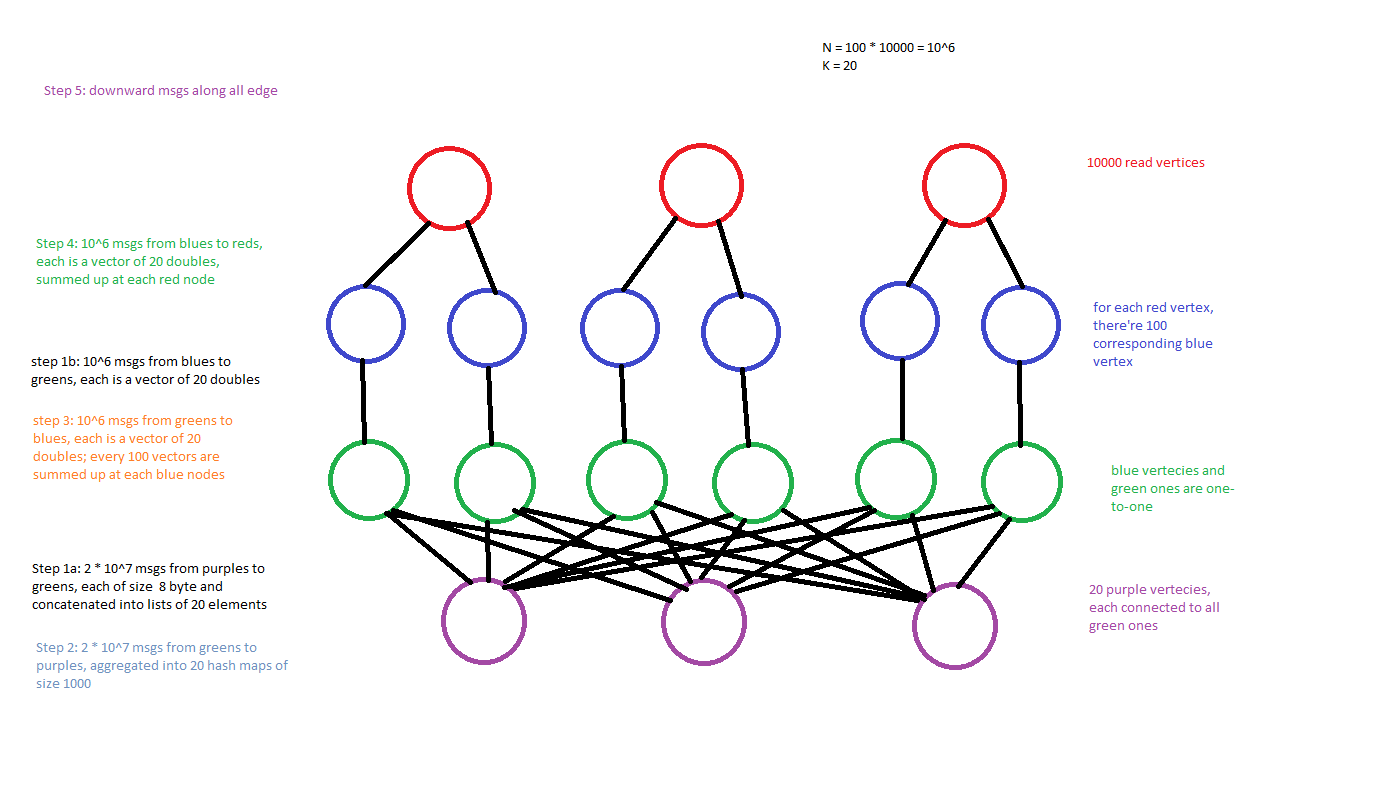
\includegraphics[scale=0.5]{lda.png}
%	\caption{Unrolled LDA bayesian network (TODO replace this with TSM)}
%\end{figure*}


%\section{Experimental Results}
\label{sec:eval}
In this section, we first present the data set, 
then compare the fuzzy match results
of the ODL system with three other competing methods, before evaluating the
effects of incremental manual correction strategies.

\subsection{Dataset and Preprocessing}
%\JY{
%The dataset that we used for evaluation comes from real life ECG reports. 
%These reports come from different hospitals recorded at different times
%and they can be divided into many different formats. 
%For our experiment, we choose four different formats. 
%The examples about these formats are shown in \figref{fig:dataset}.
%One of the reason that we choose images in these four formats is 
%these four formats have the largest number of images. 
%Another reason is they contain different attributes, languages, and so on.
%}
The dataset we use are from real ECG reports, and are recorded at 
different times and different hospitals. Those reports can be 
divided into several different categories. We chose four typical kinds 
of reports which include many images and contain much useful information 
such as attributes, languages so that we could extract more data 
from them (see \figref{fig:dataset}).
% and they can be divided into four different formats with examples shown in \figref{fig:dataset}. 
The statistics about our dataset is shown in \tabref{tab:statis}. 

\begin{figure}[th]
\centering
\subfloat[Format 1]{
\label{fig:dataset:1}
\epsfig{file=figure/f1.eps, width=0.24\columnwidth}
}
% \hfill
\subfloat[Format 2]{
\label{fig:dataset:2}
\epsfig{file=figure/f2.eps, width=0.24\columnwidth}
}
%\hfill
\subfloat[Format 3]{
\label{fig:dataset:3}
\epsfig{file=figure/f3.eps, width=0.24\columnwidth}
}
\subfloat[Format 4]{
\label{fig:dataset:4}
\epsfig{file=figure/f4.eps, width=0.24\columnwidth}
}
\caption{Examples of Four Kinds of ECGs}
\label{fig:dataset}
\end{figure}

\begin{table}[th]
\centering
\caption{Statistics for The Dataset}
\label{tab:statis}
\begin{tabular}{|c|c|c|c|c|}
\hline
Format & 1 & 2 & 3 & 4\\
\hline \hline
Number of Images & 124 & 113 & 102 & 97\\ 
\hline
Number of Attributes per Image & 17 & 16 & 18 & 15 \\
\hline
\end{tabular}
\end{table}

As the examples shown, these ECG images are in different colors 
and have many noises like grid lines. 
Because these variations and noises affect the performance of the OCR engine, 
we preprocess the images into a clean version. 
The detailed techniques are discussed in \secref{sec:discuss}. 

% we use auto thresholding to 
% preprocess the images to remove the noisy lines and 
% turn the color images into black and white. 
% An example of the preprocessing result is shown in \figref{fig:preprocess}. 
% Auto thresholding is to segment the images based on the colour 
% features automatically. In our system we make use of the tool 
% ImageJ\cite{schneider2012671} to do the preprocessing.  
% \begin{figure}[ht]
% \centering
% \subfloat[Before Preprocessing]{
% \label{fig:preprocess:1}
% \epsfig{file=figure/f1.eps, width=0.48\columnwidth}
% }
% % \hfill
% \subfloat[After Preprocessing]{
% \label{fig:preprocess:2}
% \epsfig{file=figure/pref1.eps, width=0.48\columnwidth}
% }
% \caption{Results of Preprocessing}
% \label{fig:preprocess}
% \end{figure}

\subsection{Extraction Accuracy}
Next, we compare our method with three competing methods.
The first and most naive method for information extraction from medical images 
is to write a simple parser for the XML results of the OCR engine. 
We consider this approach to be the baseline for 
evaluation. In this parser, we didn't include any fuzzy matching 
strategies, but instead extracted all results using exact matches. 

The second competing method involves marking all zones of interest 
on images and getting all the OCR results in them. 
To adjust the small changes of 
zone areas between images, a marker zone is set so that 
all other zones of interest can be adjusted against it as
a reference point. 
An example image after being marked with the zones of interest 
and the marker zone is shown in \figref{fig:zOCR} (Zones of interest 
are in blue and the marker zone is in red).

\begin{figure}[th]
\begin{minipage}{0.5\columnwidth}
\centering
\epsfig{file=figure/17_zOCR.eps, width=0.7\columnwidth}
\caption{Image Marked With Zones}
\label{fig:zOCR}
\end{minipage}
\begin{minipage}{0.5\columnwidth}
\centering
\epsfig{file=figure/17_pl.eps, width=0.7\columnwidth}
\caption{Page Layout Analysis Result}
\label{fig:pl}
\end{minipage}
\end{figure}

The third approach is to use the page layout analysis 
technique \cite{o1993document}. 
This method is used to determine where the text 
resides on a page. 
By this method, the hierarchy of physical components 
can be generated against which we can match the predefined 
hierarchy of logical components. An example result of our page layout 
analysis is shown in \figref{fig:pl}.

\begin{figure}[th]
\centering
\epsfig{file=figure/2_pl.eps, width=0.5\columnwidth}
\caption{An Error Page Layout Analysis Result}
\label{fig:errorpl}
\end{figure}


The results of comparison are shown in \tabref{tab:compare}. 
We only calculated the accuracies for extracting the results of 
variables since we already know the exact values of constant 
expressions. Based on our experiment, our method of fuzzy matching 
outperforms all other methods on all 4 types of ECGs. 
The reason is that zonal OCR and page layout analysis are highly 
related to image processing in order to extract data. The accuracy of 
zonal OCR is greatly affected by the setting of zones of interest. 
If the zones of interest are too large, it's possible that noises are
also extracted; while if the zones of interest are too small, results 
can be incomplete. For page layout analysis, the accuracy is 
affected by the granularity of the page layout unit and the 
misrecognition affects the matching with the predefined 
hierarchy of logical components. For our method, the smallest 
unit is word in text so our description can be very accurate. 
At the same time, the fuzzy matching strategies also enable 
the description to omit some unnecessary details.
% \KZ{Need focus on explaining why we are only slightly better, and what are
% the problems of the other three methods, despite that their accuracies are
% not that bad! e.g., efforts to mark the zones, I'm still not convinced
% how come without fuzzy match, zonal methods can be so good since the dist
% between the marker zone and the interesting zones can be slightly off in each
% image.}   

Even though the two competing approaches seem just marginally outperformed
by our fuzzy matching approach, these two approaches have their own 
important limitations. 
In a zonal OCR, it's important to adjust the zones of interest 
based on the marker zone. Misrecognition of the marker 
is disasterous, as all the extracted information will be incorrect. 
The other approach, page layout analysis, requires analyzing 
the text boxes in images before conducting logical labeling. 
If the text boxes are recognized incorrectly, some of the
important information may be omitted from output. 
As shown in \figref{fig:errorpl}, 
text box recognition errors cause the OCR to overlook the unit and 
other valuable information. 
However, the fuzzy match design of our system can 
tolerate these types of errors that the OCR engine often makes. 
We seek to find an optimized solution which can extract 
correct information as much as possible. 


\begin{table}[th]
\centering
\caption{Accuracy For Different Methods}
\label{tab:compare}
\begin{tabular}{|c|c|c|c|c|}
\hline
Format & 1 & 2 & 3 & 4\\
\hline \hline
Exact Match & 58.8\% & 56.3\% & 61.1\% & 53.4\% \\
\hline
Zonal OCR & 81.2\% & 79.8\% & 81.7\% & 80.6\% \\
\hline
Page Layout & 79.7\% & 80.2\% & 81.2\% & 81.1\% \\
\hline
Our Fuzzy Match & {\bf 85.5\%} & {\bf 83.8\%} & {\bf 84.9\%} & {\bf 84.0\%}\\ 
\hline
\end{tabular}
\end{table}

\subsection{Incremental Manual Correction}
%In this section, we compare the performance of 
%the human correction part in our system. 
%Another important part of our system is the human correction 
%process. By making use of the human power, we can correct 
%the errors that occur due to the OCR engine. 
We compare the two policies for recommending errors for manual correction, 
namely, random recommendation and most frequent error 
description element recommendation. The relationship between the 
amount of corrections and the accuracy of different types of 
ECGs are shown in \figref{fig:humancorr}. 
%For random correction, we randomly suggest that some errors be 
%corrected each time. 
%The accuracy of random correction is calculated by averaging 
%the results 100 times. For the most frequent error 
%description element recommendation, 
%corrections for most frequently made errors will be suggested first. 

%\KZ{Some of the words are incorrectly displayed in the following figures.}

\begin{figure}[!ht]
\centering
\subfloat{
%% \label{fig:hc:1}
\epsfig{file=figure/hcf1.eps, width=0.48\columnwidth}
}
% \hfill
% \centering
\subfloat{
% \label{fig:hc:2}
\epsfig{file=figure/hcf2.eps, width=0.48\columnwidth}
}
\hfill
% % \centering
\subfloat{
% \label{fig:hc:3}
\epsfig{file=figure/hcf3.eps, width=0.48\columnwidth}
}
% % \centering
\subfloat{
% \label{fig:hc:4}
\epsfig{file=figure/hcf4.eps, width=0.48\columnwidth}
}
\caption{Comparison of Two Correction Strategies in 4 Types of Images}
\label{fig:humancorr}
\end{figure}

% \KZ{Need to modify the figs so that lines don't touch into
% the legends, ad the caption don't overlap with the figs.}

As shown in \figref{fig:humancorr}, the more corrections we make, 
the better accuracy we get. 
The improvement to the accuracy rate is better 
when using the most frequent recommendation, compared with random 
recommendation. Using the most 
frequent recommendation is more effective, 
since we can correct more errors than random recommendation. 
With more corrections made, the improvement of 
accuracy tends to saturate, especially with regard to the 
most frequent error strategy. This is the effect of diminishing
returns, as corrections learned later tend to be minor ones and make
less impact to the overall performance.
% \KZ{Need to explain why there's only limited improvement after 15 corrections.
% Maybe because the data size is not big enough, so there's not many repeated
% errors?}
The improvement of accuracy is limited after 15 corrections. 
The main reason is that there are not many repeated errors due to 
the small size of the data set and furthermore, our system 
can only make corrections according to the correction model, 
which is sensitive to repeated errors.

% \begin{enumerate}
% \item Compare the description code with generated code to show our language is a simple one;
% \item Compare the accuracy with baseline, exact match on the OCR results, to show our language can tolerate the noises and errors;
% \item Compare the performance on different image formats;

% \item Compare the accuracy between our approach and others, including using related image position;


% \item Experiments about the relationship of the accuracy rate 
% and the number of errors corrected;

% \begin{table}[!hbp]
% \centering
% \caption{Most Frequent}
% \begin{tabular}{|c|c|c|c|c|}
% \hline
% Type & 1 & 2 & 3 & 4\\
% \hline
% Accuracy(0 errors) & 85.5\% & 83.8\% & 84.9\% & 84.0\%\\ 
% \hline
% Accuracy(1 errors) & 85.7\% & 84.0\% & 85.0\% & 84.2\%\\ 
% \hline
% Accuracy(5 errors) & 86.2\% & 84.6\% & 85.6\% & 84.8\% \\
% \hline
% Accuracy(10 errors) & 86.6\% & 85.2\% & 86.2\% & 85.5\% \\
% \hline
% Accuracy(15 errors) & 86.8\% & 85.7\% & 86.6\% & 85.9\% \\
% \hline
% % \caption{Most Frequent}
% \end{tabular}
% \end{table}

% 0 85.5 85.5
% 1 85.7 85.5
% 5 86.2 85.7
% 10 86.6 86.0
% 15 86.8 86.2

% 0 83.8 83.8
% 1 84.0 83.9
% 5 84.6 84.1
% 10 85.2 84.4
% 15 85.7 84.7

% 0 84.9 84.9
% 1 85.0 84.9
% 5 85.6 85.1
% 10 86.2 85.4
% 15 86.6 85.7

% 0 84.0 84.0
% 1 84.2 84.1
% 5 84.8 84.4
% 10 85.5 84.7
% 15 85.9 85.1

% \begin{table}[!hbp]
% \centering
% \caption{Random}
% \begin{tabular}{|c|c|c|c|c|}
% \hline
% Type & 1 & 2 & 3 & 4\\
% \hline
% Accuracy(0 errors) & 85.5\% & 83.8\% & 84.9\% & 84.0\%\\ 
% \hline
% Accuracy(1 errors) & 85.5\% & 83.9\% & 84.9\% & 84.1\%\\ 
% \hline
% Accuracy(5 errors) & 85.7\% & 84.1\% & 85.1\% & 84.4\% \\
% \hline
% Accuracy(10 errors) & 86.0\% & 84.4\% & 85.4\% & 84.7\% \\
% \hline
% Accuracy(15 errors) & 86.2\% & 84.7\% & 85.7\% & 85.1\% \\
% \hline
% % \caption{Random}
% \end{tabular}
% \end{table}


% \begin{figure}
% \centering
% \subfloat[ECG1]{
% \label{fig:hcre:a}
% \epsfig{file=figure/f1.eps, width=0.48\columnwidth}
% }
% \hfill
% \subfloat[ECG2]{
% \label{fig:hcre:b}
% \epsfig{file=figure/f2.eps, width=0.48\columnwidth}
% }
% \hfill
% \subfloat[ECG3]{
% \label{fig:hcre:c}
% \epsfig{file=figure/f3.eps, width=0.48\columnwidth}
% }
% \hfill
% \subfloat[ECG4]{
% \label{fig:hcre:d}
% \epsfig{file=figure/f4.eps, width=0.48\columnwidth}
% }
% % \caption{E}
% \label{fig:hcre}
% \end{figure}

% \item Compare different strategies for correcting errors, including most frequent error elements, most frequent error types.
% \end{enumerate}

%%!TEX root = paper.tex

\section{Related Work}
\label{sec:related}

MLlib, Mahout \cite{mahout}, and MADLib \cite{madlib} are machine learning \emph{libraries} on top of distributed computing platforms and relational engines.
All of them provide many standard machine learning models such as LDA and SVM.
However, when a domain user, say, a machine learning researcher, 
is devising and testing her customized models with her big data, 
those libraries cannot help.

MATLAB and R have been the most popular systems for implementing inference algorithms.
They, however, can hardly scale up when faced with increasing amount of data
because they mostly work on a single machine and thus cannot easily scale out.
It is possible to first transform a large dataset into a smaller one
using MapReduce or Spark and then load the data to MATLAB or R to perform inference %on the smaller ones in
in some scenarios. But this approach involves multiple systems, which is hard to
develop code for and inefficient because of the data movement.
SystemML \cite{systemml} provides a similar interface for implementing inference
algorithms and transforms them to Hadoop MapReduce. It can scale out to large
clusters but coding on such a system still requires extensive knowledge in
statistical inference for end-user. 

In contrast to the systems above, MLBase \cite{mlbase} targets end-users who are not
machine learning experts. It exposes a declarative language interface and
provides a cost-based optimizer that selects the best algorithm and
parameters. It also provides MLI \cite{mli}, a set of APIs for customizing algorithms on
Spark. However, MLBase mainly supports frequentist approach, such as SVM,
and logistic regression. It does not deal with general Bayesian inference. 

There are a number of probabilistic programming frameworks other than
Infer.NET \cite{InferNET14}.  For example, Church \cite{GMR+08} is a
probabilistic programming language based on the functional programming
language Scheme.  Church programs are interpreted rather than compiled.
Random draws from a basic distribution and queries about the execution trace
are two additional type of expressions. A Church expression defines a
generative model. Queries of a Church expression can be conditioned on any
valid Church expressions. Nested queries and recursive functions are also
supported by Church. Church supports stochastic-memoizer which can be used to
express nonparametric models.  Despite the expressive power of Church, it
cannot scale for large dataset and models.  Figaro is a probabilistic
programming language implemented as a library in Scala \cite{Figaro}.  It is
similar to Infer.NET in the way of defining models and performing inferences
but put more emphasis to object-orientation. Models are defined by composing
instances of Model classes defined in the Figaro library.  Infer.NET is a
probabilistic programming framework in C\# for Bayesian Inference. A rich set
of variables are available for model definition. Models are converted to a
factor graph on which efficient built-in inference algorithms can be applied.
Infer.NET is the best optimized probabilistic programming frameworks so far.
Unfortunately, all existing probabilistic programming frameworks including
Infer.NET cannot scale out on to a distributed platform.

To the best of our knowledge, InferSpark is the only framework that can
efficiently carry out large-scale Bayesian inference through probabilistic
programming on a distributed in-memory computing platform. It targets
end-users who are not expert in Bayesian inference or distributed computing.
The inference implementation can scale out to a large cluster and scale up to
large datasets.

%
%Our proposed probabilistic programming language is also an extension to the existing language Scala, but differs from the way that Infer .NET and Figaro define models that we add additional language constructs to Scala rather than implement a library. It typically enables a cleaner syntax. 







%\item Other inference algorithms for Bayesian Networks.



\cut{%%%%%%%%%%%%%%
The Apache Hadoop library \cite{hadoop} is a distributed data storage and processing framework. Its distributed file system HDFS support the storage of large data. MapReduce is the programming model for distributed parallel processing of the large data. It is composed of two key operations map and reduce. Map operation transforms and filters the data on different nodes in parallel while reduce operations combines the results from map operation to produce results grouped by keys. In our proposal of PP, data can be distribted on a HDFS.

Spark is another distributed data processing framework that provides MapReduce operations. It differs from Hadoop in that it does not write the intermediate results to temporary storage. Instead, it caches the results in memory as resilient distributed dataset \cite{Zaharia:2012:RDD:2228298.2228301}. It can greatly speed up the processing. 

The Spark built-in machine learning library MLlib \cite{mllib} provides a variety of standard statistical inference algorithms including classification, regression, clustering, collaborative filtering and dimensionality reduction. The algorithms leverage the Spark infrastructure so that large-scale data can be processed efficiently. The algorithms are applicable when the standard models fit the data well. Users have to directly develop their own algorithms using Spark or GraphX API when a customized model has to be used. Our integration of PP with Spark can greatly reduce the amount of work to implement a new model.

GraphX \cite{Xin:2013:GRD:2484425.2484427} is Spark's built-in graph parallel computation API. User can view graphs as normal RDDs of vertices and edges and perform normal map reduce operations on them or perform graph operations like compute subgraph, reversing edges, join vertices. The Pregel operator in GraphX is used to express iterative algorithms. In each step, vertices aggregates messages along the inbound edges from previous step, compute its new value and sends messages along outbound edges in parallel. It terminates when no message is sent during a step. Our PP will be built on GraphX since it is natural to represent the factor graph in GraphX and leverage the parallel graph computing to implement message-passing style inference algorithms.

\KZ{Reduce the discussion of the following PP languages a bit. Focus on
their big-data handling capabilities, or the lack of which.}

Many recent probabilistic programming languages are implemented by extending existing conventional programming languages such as Scheme, C\#, Scala and etc.
We examine three probabilistic programming languages Church \cite{GMR+08}, Infer .NET \cite{InferNET14} and Figaro \cite{pfeffer2009figaro}.

Church is a probabilistic programming language based on the functional programming language Scheme. Random draws from a basic distribution and queries about the execution trace are two additional type of expressions. A church expression defines a generative model. Queries of a church expression can be conditioned on any valid church expressions. Nested queries and recursive functions are also supported by Church. Church supports stochastic-memoizer which can be used to express nonparametric models. Thus a wide range of probabilistic models can be concisely expressed in Church. Inference in Church is implemented by rejection sampling and Metropolis-Hastings sampling algorithms. Despite the expressive power of Church, it cannot scale up to large dataset and models. 

Our approach differs from Church in that our program is compiled rather than interpreted. Compiled program is usually more efficient than interpreted ones. We can also leverage the distributed parallel processing to scale up to large dataset and models.

Infer .NET is a probabilistic programming framework in C\# for Bayesian Inference. A rich set of variables are available for model definition. Models are converted to a factor graph on which efficient built-in inference algorithms can be applied. The algorithms include expectation propagation, variational message passing, block Gibbs sampling. Infer .NET addresses the scalability by shared variables, as discussed in Section \ref{sec:intro}.
%% ?? not sure about how the shared variable is implemented

Figaro is a probabilistic programming language implemented as a library in Scala. It is similar to Infer .NET in the way of defining models and performing inferences but put more emphasis to object-orientation. Models are defined by composing instances of Model classes defined in the Figaro library.

Our proposed probabilistic programming language is also an extension to the existing language Scala, but differs from the way that Infer .NET and Figaro define models that we add additional language constructs to Scala rather than implement a library. It typically enables a cleaner syntax. 

}%%%%%%%%%%%%%%%%

%\section{Conclusion}

In this paper, we incorporated the idea of Cookie Theft picture description task into the evaluation of the high-level cognitive abilities of LVLMs and designed a novel evaluation benchmark called CogBench.
% Images in CogBench are of high quality and require more cognitive reasonings to understand, which makes it different from existing image datasets.
The images in CogBench are of high quality and demand more complex cognitive reasoning for interpretation, setting it apart from existing image datasets.
% It consists of a image description task and a VQA task.
Experiments show that there is still a large gap between the cognitive abilities of LVLMs and human beings, indicating CogBench is a challenging benchmark.

% In the future

%\subsection{Future Directions}
\label{sec:future}


We discuss some possible future directions and organize them into
three dimensions: \textit{task scenarios}, \textit{approaches} and \textit{evaluations}. 


\subsubsection{More Complicated and Controllable Scenarios}

Newly explored scenarios such as multi-lingual, multi-modal, multi-session and personalized dialogue summarization are worth researching.
%In addition, we put forward {personalized dialogue summarization} as a novel future direction that pays special attention to speaker or reader-related information neglected by previous works.

\textbf{Multilingual dialogue summarization} is a rising topic. It considers multiple languages existing in the dialogue and summary on three levels of granularity. The most fine-grained one considers interactions between peers who are fluent in multiple languages resulting in the intra-utterance multilingual phenomenon is called ``code-mixing'' strictly~\cite{mehnaz2021gupshup}. Second, dialogues happening among multinational participants where they use their mother tongue to communicate lead to the inter-utterance multilingual phenomenon is called ``code-switching''~\cite{mehnaz2021gupshup}, i.e., mix-lingual in~\cite{feng2022msamsum}. Third, summarizing a monolingual dialogue in a different language is called ``cross-lingual'' in~\citet{wang2022clidsum}. Different multilingual datasets have been constructed for these settings based on the existing datasets~\cite{gliwa2019samsum, chen2021dialsumm,zhu2021mediasum,zhong2021qmsum} by human annotations~\cite{wang2022clidsum,mehnaz2021gupshup,chen2022cross} or machine translation~\cite{feng2022msamsum}. Preliminary studies in these papers show the potential of end-to-end multilingual models, such as mBART~\cite{tang2021multilingual},  in this task and their weaknesses in low-resource languages, poor domain transfer ability~\cite{wang2022clidsum} and performance drops when processing multiple languages with a single model~\cite{feng2022msamsum}. \citet{chen2022cross,chen2023revisiting} proposed the cross-lingual conversation summarization challenge, paving the way for the prosperity of research in this direction. Our survey focuses on approaches for monolingual dialogue summarization, which we expect to provide a backbone for this raising area.



\textbf{Multi-modal dialogue summarization} refers to dialogues occurring in 
multi-modal settings, which are rich in non-verbal information 
that often complements the verbal part and therefore contributes to 
summary contents. Some early work did research on speech dialogue summarization. 
However, most of them only extract audio features from speech and text 
features from ASR transcripts independently to produce extractive summaries. 
There is also work on video summarization~\cite{hussain2021video} focusing 
on highlighting critical clips while a textual summary is not considered.
Fusing the synchronous and asynchronous information among modalities 
is challenging. AMI and ICSI are still valuable resources for 
research on multi-modal dialogue summarization.



\textbf{Multi-session dialogue summarization} is required when conversations 
occur multiple times among the same group of speakers. 
The Information mentioned in previous sessions becomes their consensus and 
may not be explained again in the current session. 
The summary generated merely from the current session is unable to 
recover such information and may lead to implausible reasoning. 
A similar multi-session task has been proposed by~\citet{xu2021beyond}. 
This setting also has some correlations with life-long learning~\cite{liu2021lifelong}.
Such multi-session dialogues exists in ODS datasets, such as SubTitles~\cite{malykh2020sumtitles} and SummScreen~\cite{chen2021summscreen}. However, current approaches generally break down the long dialogue and summary into shorter chunks. 
For task-oriented scenarios, it is also common in real life. For example, the customer may repeatedly ask for help from the agent with the same issue that hasn't been solved before. An updated summary covering the questions and answers can remind participants of the long dialogue history and therefore facilitate the negotiation process. 



Recent work mainly focuses on summarizing the dialogue content but ignores the speaker-related or reader-related information. 
\textbf{personalized dialogue summarization} can be understood in two ways. 
On the one hand, a personalized dialogue refers to the consideration of 
personas for interlocutors in dialogues. For example, the character 
role-playing information is indispensable information for generating 
summaries given dialogue from CRD3~\cite{rameshkumar2020storytelling}.
On the other hand, it refers to generating different dialogue summaries for 
different readers or speakers. \citet{tepper2018personal} is a demo paper raising the 
requirements for personalized chat summarization. They did the first trial 
on this task considering the personalized topics of interests and social ties 
during the selection of dialogue segments to be summarized. 
Some task-oriented datasets, such as CSDS~\cite{lin2021csds}, contain summaries from both the user and agent aspect are similar
to the problem here. Recent work from~\citet{lin2022other} solved this problem by adding the cross attention interaction and the decoder self-attention interaction to interactively acquire other roles' critical information. This work is designed only for scenarios with two roles.
Scenarios with a variety number of speakers and summary readers from different social groups pose more challenges, raising an
expectation for related datasets and approaches, which is a possible interdisciplinary research orientation.


\subsubsection{Innovations in Approach} 
Approach innovations include four parts:  feature analysis, person-related features, generalizable and non-labored techniques, and the robustness of models.

From \secref{sec:observations}, although tens of papers 
introduce different features for dialogue summarization, there is still 
a lot of work to do. Comprehensive experiments to \textbf{compare the} \textbf{features} and 
their combinations upon the same benchmark are expected, 
for features both in the same category or across categories. 
One can consider unifying the definition of similar features, 
e.g., different classification criteria of discourse relations or graphs emphasizing phrase-level semantic flows. 
These analyses would help design features for new applications and interpret dialogue models.
%It's also \KZ{substantial for explanations of dialogue modeling, and also helpful for feature selection} in new applications. 


More \textbf{person-related features} can be incorporated, 
such as speaker personalities~\cite{zhang2019consistent} and 
emotions~\cite{majumder2019dialoguernn}. A speaker's background can help understand the underlying motivation and select the content to be summarized, especially for personalized dialogue summarization.
A plug-and-play mechanism on top of the decoder for persona-controlled summarization may be a solution~\cite{DathathriMLHFMY20}.
 



\textbf{Generalizable and non-labored techniques} have attracted increasing attention on other dialogue modeling tasks, 
such as multi-turn response selection~\cite{xu2021learning} and 
dialogue generation~\cite{zhang2019consistent}. 
These works proposed different self-supervised training tasks, largely relieving human labor.
However, dialogue summarization approaches overwhelmingly 
rely on injecting pre-processed features, which are mostly labor-intensive and has poor generalization ability among scenarios.
Recently, large language models~(LLMs) with tons of billions of parameters like GPT-3~\cite{brown2020language} and LLaMA~\cite{touvron2023llama} have demonstrated drastically lifted text generation ability compared to previous pre-trained language models. To accomplish summarization task, LLMs are typically prompted with instructions like ``\textit{Summarize the above article:}'' or chain-of-thought~\cite{cot,wang-etal-2023-element} methods that elicit LLMs to extract various features, e.g., events, that are helpful to compose the final summary. Compared with traditional methods, LLM-based methods largely alleviate the tedious human labor and can be more generalizable due to the removal of unintended annotation artifacts. Nevertheless, approaches previously applied to small pre-trained language models may also provide inspirations and be adapted to augment LLMs for better dialogue summarization performance.

Approaches nowadays are mostly built on the pre-trained language models, which are sensitive to trivial changes~\cite{wang-etal-2022-rely,yan2022robustness}. 
Nevertheless, the \textbf{robustness of models} hasn't been widely-investigated in dialogue summarization. The only work from~\citet{jia2023reducing} proposed that switching an un-grounded speaker name shouldn't influence the models' generation. According to their experiments with BART fine-tuned on SAMSum, such changes can lead to dramatically different summaries with information divergence and various reasoning results. This may further result in unintended ethical issues by showing discrimination against specific groups of names. Thus, analysis and improvements of models' robustness are in urgent need for practical applications.



\subsubsection{Datasets and Evaluation Metrics}
Expectations on datasets and evaluation metrics for dialogue summarization are as follows.

\secref{sec:observations} shows that \textbf{high-quality datasets} 
expedite the research. Besides the expectations on benchmark datasets for the above emerging scenarios, datasets for task-oriented dialogue summarization 
with privacy issues are also sought after. They can be in small sizes with 
real cases after anonymization or can be collected by selecting 
drama conversations in specific scenarios and annotated with 
domain experts. 

\textbf{Evaluation metrics} are significant which guides the improvement directions for upcoming models. However, 
widely used evaluation metrics in Sec.~\ref{sec:evalmetric} are all borrowed from document summarization 
tasks and their effectiveness is unverified.
Recent work from~\citet{gao2022dialsummeval} re-evaluated 18 evaluation metrics and did a unified human evaluation with 14 dialogue summarization models on SAMSum dataset. 
Their results not only show the inconsistent performances of metrics between document summarization and dialogue summarization, and none of them excel in all dimensions for dialogue summarization, but also raise a warning on rethinking whether recently proposed complex models and fancy techniques truly improve the backbone language model.
Considering that human evaluation results are difficult to reproduce due to variations of annotator background and unpredictable situations in the annotation progress~\cite{clark2021all},
automatic metrics specially designed for dialogue summarization are urgently needed.


Factual errors caused by the mismatch between speakers and events are 
common as a result of complicated discourse relations among utterances 
in dialogues. \citet{tang2021confit} introduced a taxonomy of factual errors for abstractive summarization and did human evaluation based on this categorization. \citet{liu2021controllable} made the first attempt by inputting the 
dialogue and summary together into a BERT-based classifier and claimed 
high accuracy on their own held-out data. \citet{wang2022analyzing} classified factual errors in a similar way to~\citet{tang2021confit} and propose a model-level evaluation schema for discriminating better summarization models, which is different from the widely-accepted sample-level evaluation schema that scores generated summaries. They evaluated the model by calculating the generation probability of faithful and unfaithful summaries collected by rule-based transformations. The generalization ability for this work is doubtful, since a similar work, FactCC~\cite{kryscinski2020evaluating}, which is a metric trained based on rule-based synthetic datasets shows a poor generalization ability~\cite{laban2022summac}. With the strong generation ability of current LLMs, there's another doubt that whether the previous taxonomy of error types and evaluation metrics are still suitable.
In a word, both \textbf{meta-evaluation benchmarks} and \textbf{evaluation methods} call for innovations.





{
\scriptsize
\bibliographystyle{abbrv}
\bibliography{pp}
}

%\appendix
%\subsection{Syntax}
\label{sec:syntax}
% Describe the syntax of the description language.
% \begin{enumerate}
% \item Syntax for the description language, including CFG and type 
% system;
% \item Emphasize the description about spatial information (differences with pads) and constrains;
% \item Description examples.
% \end{enumerate}

%In this section, we briefly describe what an ODL data description looks like by presenting some illustrative examples. 
%
% \newsavebox{\absfalign}
% \begin{lrbox}{\absfalign}
% % \fontsize{6pt}{7pt}\selectfont
% \begin{align*}
% \text{int} ::= ~&[-+]?[0-9]+ \\
% \text{float} ::= ~&[-+]?[0-9]*.[0-9]+ \\
% \text{num} ::= ~&int|float\\
% \text{len} ::= ~&num ~~ (pixel|cm) \\
% \text{coord} ::= ~&\langle len_1, ~~ len_2, ~~ len_3, ~~ len_4\rangle \\
% \text{bop} ::= ~&+|-|*|/|=|!=|<|>|<=|>=\\
% % \text{datatype} ::=
% % ~&Oint(int, int)\\
% % |~& Ofloat(int, int, int, int)\\
% % |~& Ostring(string)\\
% \text{Value v} ::=
% ~&() \\
% |~& int \\
% |~& float \\
% |~& string \\
% |~& len \\
% |~& coord \\
% % |~& {v_1, ~~ ..., ~ v_n}\\
% %|~& \{v_1 | v_2 | ... | v_n\}\\
% |~& \{v_1, ..., v_n\} \\
% \end{align*}
% \end{lrbox}

% \newsavebox{\abssalign}
% \begin{lrbox}{\abssalign}
% % \fontsize{6pt}{7pt}\selectfont
% \begin{align*}
% \text{Expression e} ::=
% % |~& datatype ~~ x \tag{variable}\label{syntax:variable}\\
% ~&c \tag{constant}\label{syntax:constant}\\
% |~& x \tag{name}\label{syntax:name}\\
% % |~& nop ~~ e\\
% |~& e_0(e_1, e_2, ..., e_n) \tag{constraints} \label{syntax:constraints}\\
% % |~& \lambda x.e \tag{funciton}\label{syntax:function}\\
% % |~& e_1 ~~ e_2 \tag{apply}\label{syntax:apple}\\
% |~& hskip ~~e \tag{horizontal skip}\label{syntax:hskip}\\
% |~& vskip ~~e \tag{vertical skip}\label{syntax:vskip}\\
% |~& \{e_1 | e_2 | ... | e_n\} \tag{union}\label{syntax:union}\\
% % |~& \{e_1, ~~ ..., ~~ e_n\}\\
% % |~& e.i\\
% |~& \{e_1, ..., e_n\} \tag{struct}\label{syntax:struct}\\
% |~& e ~~ list \tag{list}\label{syntax:list}\\
% % |~& e_1[e_2] \tag{list element}\label{syntax:listele}\\
% |~& e ~~ as ~~ x \tag{blinding}\label{syntax:blinding}\\
% |~& e_1 ~~ bop ~~ e_2 \tag{binary operation}\label{syntax:bop}\\
% \end{align*}
% \end{lrbox}

% \begin{figure}[h]
% % \centering
% % \subfloat{\parbox{0.5\textwidth}{
% % {\usebox\absfalign}
% \begin{align*}
% \text{int} ::= ~&[-+]?[0-9]+ \\
% \text{float} ::= ~&[-+]?[0-9]*.[0-9]+ \\
% \text{num} ::= ~&int|float\\
% \text{len} ::= ~&num ~~ (pixel|cm) \\
% \text{coor} ::= ~&\langle len_1, ~~ len_2, ~~len_3, ~~ len_4\rangle \\
% \text{bop} ::=
% ~&+|-|*|/\\
% |~& =|!=\\
% |~& <|>|<=|>=\\
% % \text{datatype} ::=
% % ~&Oint(int, int)\\
% % |~& Ofloat(int, int, int, int)\\
% % |~& Ostring(string)\\
% \text{v} ::=
% ~&() \\
% |~& int \\
% |~& float \\
% |~& string \\
% |~& len \\
% |~& coor \\
% % |~& {v_1, ~~ ..., ~ v_n}\\
% %|~& \{v_1 | v_2 | ... | v_n\}\\
% |~& \{v_1, ..., v_n\} \\
% % a = b\\
% % \end{align*}
% % }}
% % \end{subfloat}
% % \hfill
% % \subfloat{
% % \subfloat{\parbox{0.5\textwidth}{
% % {\usebox\abssalign}
% % \begin{align*}
% \text{e} ::=
% % |~& datatype ~~ x \tag{variable}\label{syntax:variable}\\
% ~&c \tag{constant}\label{syntax:constant}\\
% |~& x \tag{name}\label{syntax:name}\\
% % |~& nop ~~ e\\
% |~& e_0(e_1, e_2, ..., e_n) \tag{constraints} \label{syntax:constraints}\\
% % |~& \lambda x.e \tag{funciton}\label{syntax:function}\\
% % |~& e_1 ~~ e_2 \tag{apply}\label{syntax:apple}\\
% |~& hskip ~~e \tag{horizontal skip}\label{syntax:hskip}\\
% |~& vskip ~~e \tag{vertical skip}\label{syntax:vskip}\\
% |~& \{e_1 | e_2 | ... | e_n\} \tag{union}\label{syntax:union}\\
% % |~& \{e_1, ~~ ..., ~~ e_n\}\\
% % |~& e.i\\
% |~& \{e_1, ..., e_n\} \tag{struct}\label{syntax:struct}\\
% |~& e ~~ list \tag{list}\label{syntax:list}\\
% % |~& e_1[e_2] \tag{list element}\label{syntax:listele}\\
% |~& e ~~ as ~~ x \tag{blinding}\label{syntax:blinding}\\
% |~& e_1 ~~ bop ~~ e_2 \tag{binary operation}\label{syntax:bop}\\
% % c = d\\
% % \text{Expression e} ::=
% % % |~& datatype ~~ x \tag{variable}\label{syntax:variable}\\
% % ~&c\\
% % |~& x\\
% % % |~& nop ~~ e\\
% % |~& e_0(e_1, e_2, ..., e_n)\\
% % % |~& \lambda x.e \tag{funciton}\label{syntax:function}\\
% % % |~& e_1 ~~ e_2 \tag{apply}\label{syntax:apple}\\
% % |~& hskip ~~e\\
% % |~& vskip ~~e\\
% % |~& \{e_1 | e_2 | ... | e_n\}\\
% % % |~& \{e_1, ~~ ..., ~~ e_n\}\\
% % % |~& e.i\\
% % |~& \{e_1, ..., e_n\}\\
% % |~& e ~~ list\\
% % % |~& e_1[e_2] \tag{list element}\label{syntax:listele}\\
% % |~& e ~~ as ~~ x\\
% % |~& e_1 ~~ bop ~~ e_2\\
% \end{align*}
% % }}
% % \end{subfloat}
% \caption{Syntax}
% \label{fig:syntax}
% \end{figure}

\begin{figure*}[!ht]
%\small
%\setlength{\abovecaptionskip}{0.cm}
%\setlength{\belowcaptionskip}{-0.cm}
%\scalebox{0.5}{
\begin{minipage}{0.8\columnwidth}
\begin{align*}
%\text{int} ::=~& \land-?\backslash d+\$\\
%\text{float} ::=~& \land(-?\backslash d+)(.\backslash d+)?\$\\
\text{num} ::=~& int|float\\
\text{len} ::=~& num  (pixel|l|w) ~~ | ~~ \backslash s ~~ | ~~ \backslash n\\
\text{coor} ::=~& \langle len_1, len_2, len_3, len_4\rangle\\
\text{bop} ::=
~& +|-|*|/|\%\\
|~&=|!=|<|>|<=|>=\\
% \text{datatype} ::=
% ~&Oint(int, int)\\
% |~& Ofloat(int, int, int, int)\\
% |~& Ostring(string)\\
\text{c} ::=~& ()~ |~ int~ |~ float~ |~ string \\
% |~& len \\
% |~& coor \\
% |~& {v_1, ~~ ..., ~ v_n}\\
%|~& \{v_1 | v_2 | ... | v_n\}\\
%|~& \{v_1, ..., v_n\} \\
\end{align*}
\end{minipage}
%\scalebox{0.5}{
\begin{minipage}{0.8\columnwidth}
\begin{align*}
\text{e} ::=
% |~& datatype ~~ x \tag{variable}\label{syntax:variable}\\
~& c \tag{constant}\label{syntax:constant}\\
|~& x \tag{variable}\label{syntax:name}\\
% |~& nop ~~ e\\
% |~& \lambda x.e \tag{funciton}\label{syntax:function}\\
% |~& e_1 ~~ e_2 \tag{apply}\label{syntax:apple}\\
|~& hskip ~~len \tag{horizontal skip}\label{syntax:hskip}\\
|~& vskip ~~len \tag{vertical skip}\label{syntax:vskip}\\
|~& \{e_1 | e_2 | ... | e_n\} \tag{union}\label{syntax:union}\\
|~& \{e_1, ..., e_n\} \tag{struct}\label{syntax:struct}\\
|~& e ~~ list \tag{list}\label{syntax:list}\\
% |~& e_1[e_2] \tag{list element}\label{syntax:listele}\\
|~& e ~~ as ~~ x \tag{binding}\label{syntax:binding}\\
|~& e_1 ~~ bop ~~ e_2 \tag{binary operation}\label{syntax:bop}\\
|~& e_0(e_1, e_2, ..., e_n) \tag{constraint} \label{syntax:constraints}\\
\end{align*}
\end{minipage}
\caption{Syntax of OCR description language.}
\label{fig:syntax}

\end{figure*}

% \KZ{Make \figref{fig:syntax} double column and more compact.}


%\subsubsection{Example}
%The examples we are using are shown in \secref{sec:appro}. Those are the ECG images in the real life 
%and we want to extract the time, the values for different tests, the interperation report of the ECG and the detail parameters in drawing the ECG. The ODL description for \figref{fig:ecgexample1} and \figref{fig:ecgexample2} is shown in \figref{fig:absdes} by using the abstract syntax. The out layer of the whole description is a struct expression, which combines the subdescription of four kinds of information together. 
%
% In this section, a concert example will be used to illustrate how to provide a image form description in ODL to extract information from images sharing the same form.

% For a sample ECG image \figref{fig:ecgexample}, we can write ODL description shown in \figref{fig:description}. To extract useful information from images sharing the same form. In this case, we want to extract the values for thoses four attributes on ECG. Different images will have the same name for the attributes in similar position if using similar form. So we can write the description shown in fig.
% Each line of the description is a naming expression to simply the description and the name description is used as the key word for entry of the description. 
% The out layer of the description is a struct expression provide with coordinates information. We set the coordinates of the box to avoid distributing by noises else where. The coordinates is just estimated number to make the description easy to write. In the struct named triples, we describe all important data on images and some important spational relation between them. Since thoses attributes have the form of key name, value, and optional unit. Since value differs between different images, we use variable expressions with constrains like normal range, and type. Each triples are in different line, so we use vertical skip function to indicate it. Horizontal skip function also used in order to provide detail information about layout to improve the accuracy of results.

%\subsubsection{Syntax and Type System}
% \KZ{There are still many, many typos and grammatical errors through out 
% this section and the following sections. Run a spell checker, such as aspell
% and read the sections through very carefully.}
The abstract syntax of ODL is formally described in \figref{fig:syntax}.
%\JL{
The first six types in \figref{fig:syntax} are basic types. 
%}
ODL can be used to describe both semi-structured data and 
spatial information for the physical layout. Next we 
will discuss the 
syntax and type system in more detail. 

\subsubsection{Values}

% \KZ{Discuss what types of values are there, sand it relationship with the 
% expression. Basically expression can be parsed into values. Constants
% can also be any of the values. Need to explain len, coord, etc. There's no
% such thing as $v_1$ | $v_2$ | ..| $v_n$. I removed it.}

% \KZ{Is it coor or coord? Make it consistent thruout the paper.}

Basically, all expressions in ODL can be parsed into values. Values 
in ODL can take the form of extracted textual information or the spatial parameters. 
%\JL{
	We can see that a value can take on many different shapes 
in \figref{fig:syntax}. For example, {\em ()} can be regarded as a value.
{\em int}, 
{\em float} and {\em string} can also be regarded as values.
%} 
{\em len} and {\em coor} are two special vlaue types in ODL. They indicate 
the values of spatial parameters. {\em len} contains two parameters: the  
length and the unit for the spatial description. {\em coor} {indicate  values of those
coordinates, and it contains four {\em len} values representing 
the coordinates of the top left corner and the bottom right corner of 
the region of interest (see it in \figref{fig:syntax}). The last definition for value  {\em $\{v_1, ..., v_n\}$} indicates that a struct which contains many values can also be defined as a value. 

\subsubsection{Primitive Expression}
Primitive expressions include {\em constant} and {\em name} , which are the first two definitions for expressoin.
%The idea of ODL is to describe the data information on images 
%based on the data type. 
%This idea comes from PADS, which uses types to describe ad hoc data \cite{fisher2011pads}.
%{\em Constant} and {\em name} are the basic data description 
%expressions in ODL. 
Constants represent fixed-valued strings or numerical values to be recognized from the 
image. In \figref{fig:absdes}, the key name ``Vent. rate'' and the unit 
``bpm'' for the medical test are constant expressions 
%in all ECGs of the same
%format. Constants are usually markers or delimiters in semi-structured
%data formats.

%For ECGs in the same format, the key name for the test value is always 
%``Vent. rate'' and the unit for the test value is always ``bpm''. 
On the other hand, if a data field has variable values,
but we know the data type or the constraints of the data field,
(e.g., a numeric type), we can use a {\em name}. 
In \figref{fig:absdes}, the value for ``Vent. rate'' is a variable by
the patient and their different medical tests, we use a name $x$ to represent that. 
In addition, we know that the value for ``Vent. rate'' should be an integer 
between 60 and 100, so we combine {\em name} and {\em constraints} 
to describe the whole field. 
%With the help of {\em constant} and {\em name}, ODL can be used for 
%describing a data form by using {\em constant} for shared data 
%information and {\em name} for different data on individual images.

\subsubsection{Spatial Expression}
Spatial description expressions include % {\em function}, 
{\em hskip e} and {\em vskip e}. 
These are essential constructs for ODL to describe spaces in the images. 
For ODL, an image document can be considered the combination of 
one or more text areas, or text boxes. In \figref{fig:ecgexample2}, 
there are four separate text boxes on the image. 
%In this case, we designed ODL with expressions for describing 
%this spatial information. 
In ODL, the text boxes are described by using the coordinates of 
the corners of the box. This coordinates information also serves to define 
constraints. Text boxes can be specified if we want 
to describe the layout on large scale. 
% \KZ{What's the diff between information box and text box?} 
{\em hskip e} and {\em vskip e} can be used for describing 
approximate distances horizontally or vertically. 
%So in ODL, rough spatial description can also be used to indicate 
%that there is a small space or there is a large space. 
%\JL{
%The detailed process of choosing final results with the 
%help of spatial description will be discussed later 
%in section \ref{sec:semantics}. 
%}
% Fuzzy matching the layout description with the real input 
% will be discussed later in section \ref{sec:semantics}. 
Since spatial information is usually described together with the 
measurement unit, like pixel or centimeter, 
the spatial description expression in ODL can only 
be generated with ``len'' expressions. 
In the example, the coordinates of the upper left corner and 
the bottom right corner for four main parts of the image are outlined in the 
constraints and the symbol ``\_'' means default, which means the 
coordinates of the upper left corner and the bottom right corner of the 
whole document. {\em hskip $\backslash$s} indicates that there are some spaces 
between the key ``Vent. rate'' and the value $x$. And {\em vskip $\backslash$s} 
indicates that there are some vertical spaces between information about 
interpretation and parameters. 
% \KZ{Why not also $vskip~\backslash s$?}

\subsubsection{Composition}
Composition expressions are compound expressions constructed from other
expressions. These include 
{\em union}, {\em struct}, {\em list}, 
{\em constraints}, {\em binding} and {\em bop}.

%With the help of the two kinds of expressions before, we can describe what's on the image and where are they. We combine these two parts in ODL by using complex type expressions. In the example, {\em struct}, {\em union} and {\em list} is used. 
{\em Struct} is used to describe a text box by using both data description 
expressions and spatial description expressions. 
In {\em struct}, all sub-expressions are described in a sequence, 
and the default sequence is from left to right and from top to bottom. In the struct description for ``tuples'', key, value and unit are listed from left to right. 
%Exceptions happen when the space skip function is applied to a negative number, which means moving the cursor backwards. 
{\em Union} means there are many potential data or potential spatial operations to consider. The union description for ``month'' is the enumeration of all abbreviations of the names of the months.
{\em List} is used to indicate that a sequence of similar data or the same spatial operations should be applied multiple times. In the example, {\em list} is used to indicate that there are many blank lines between descriptions for interpretation and parameters.
{\em Constraints} can  
be set based on both data description expressions and 
spatial description expressions. In ODL, constraints can be put on 
% primitive expressions or composition expressions. 
data or a text box. 
% \KZ{What's the difference between data and a text box?}
%Detailed constraints on data can be about the 
%type of the data or the value of the data, while constraints for a
%text box are coordinates that specify the spatial boundaries of the text box. 
Other expressions like {\em binding} and {\em bop} are designed to 
simplify the description and make ODL more expressive. 
The function of {\em binding} is to give a name {\em x} to 
the expression {\em e} so that we can reuse the parsing result of {\em e} 
in the latter description. 
% \KZ{Can say a bit more about what is the purpose of binding.}

% \figref{fig:ecgexample} gives an example ECG report. An ECG report 
% contains values for different attributes. 
% Those values are important for doctors to know the physical condition 
% of patients and make decisions about the treatment. 
% For most of the medical images, values of different test results 
% usually appear in the similar key-value pair format. 
% In this case, we propose ODL data description language to describe the 
% structured information on medical images easily and extract them efficiently.

% \begin{figure}[h]
% \begin{eqnarray*}
% &&\{``Vent.", ``rate", Oint ~~ valueVent, (hskip ``s"), ``bpm", (vskip ``n")\} ~~ as ~~ triples\\
% &&triples_{(imageWidth/10, default, imageWidth/2, default)} ~~ as ~~ description\\
% \end{eqnarray*}
% \caption{Description}\label{fig:description}
% \end{figure}
% % ?general description, features
% ODL uses a type system and spatial description to 
% describe data on medical images. 
% Base types describe atomic pieces of data or represent 
% spatial information and complex types describe how 
% to build compund descriptions from simpler ones. ODL 
% also use additional information to provide constrains 
% based on doctors' knowledge. 
% Besides the description of the data itself, 
% ODL provides spatial description expression to allow users 
% to descrbe the physical layout of the data on the image. 


% %syntax and examples
\subsection{Expression}
The syntax of ODL is formally described in 
\figref{fig:syntax}. An example 
description for \figref{fig:ecgexample} is show in 
\figref{fig:description}. 

% \newsavebox{\absfalign}
% \begin{lrbox}{\absfalign}
% % \fontsize{6pt}{7pt}\selectfont
% \begin{align*}
% \text{int} ::= ~&[-+]?[0-9]+ \\
% \text{float} ::= ~&[-+]?[0-9]*.[0-9]+ \\
% \text{num} ::= ~&int|float\\
% \text{len} ::= ~&num ~~ (pixel|cm) \\
% \text{coord} ::= ~&\langle len_1, ~~ len_2, ~~ len_3, ~~ len_4\rangle \\
% \text{bop} ::= ~&+|-|*|/|=|!=|<|>|<=|>=\\
% % \text{datatype} ::=
% % ~&Oint(int, int)\\
% % |~& Ofloat(int, int, int, int)\\
% % |~& Ostring(string)\\
% \text{Value v} ::=
% ~&() \\
% |~& int \\
% |~& float \\
% |~& string \\
% |~& len \\
% |~& coord \\
% % |~& {v_1, ~~ ..., ~ v_n}\\
% %|~& \{v_1 | v_2 | ... | v_n\}\\
% |~& \{v_1, ..., v_n\} \\
% \end{align*}
% \end{lrbox}

% \newsavebox{\abssalign}
% \begin{lrbox}{\abssalign}
% % \fontsize{6pt}{7pt}\selectfont
% \begin{align*}
% \text{Expression e} ::=
% % |~& datatype ~~ x \tag{variable}\label{syntax:variable}\\
% ~&c \tag{constant}\label{syntax:constant}\\
% |~& x \tag{name}\label{syntax:name}\\
% % |~& nop ~~ e\\
% |~& e_0(e_1, e_2, ..., e_n) \tag{constraints} \label{syntax:constraints}\\
% % |~& \lambda x.e \tag{funciton}\label{syntax:function}\\
% % |~& e_1 ~~ e_2 \tag{apply}\label{syntax:apple}\\
% |~& hskip ~~e \tag{horizontal skip}\label{syntax:hskip}\\
% |~& vskip ~~e \tag{vertical skip}\label{syntax:vskip}\\
% |~& \{e_1 | e_2 | ... | e_n\} \tag{union}\label{syntax:union}\\
% % |~& \{e_1, ~~ ..., ~~ e_n\}\\
% % |~& e.i\\
% |~& \{e_1, ..., e_n\} \tag{struct}\label{syntax:struct}\\
% |~& e ~~ list \tag{list}\label{syntax:list}\\
% % |~& e_1[e_2] \tag{list element}\label{syntax:listele}\\
% |~& e ~~ as ~~ x \tag{blinding}\label{syntax:blinding}\\
% |~& e_1 ~~ bop ~~ e_2 \tag{binary operation}\label{syntax:bop}\\
% \end{align*}
% \end{lrbox}

% \begin{figure}[h]
% % \centering
% % \subfloat{\parbox{0.5\textwidth}{
% % {\usebox\absfalign}
% \begin{align*}
% \text{int} ::= ~&[-+]?[0-9]+ \\
% \text{float} ::= ~&[-+]?[0-9]*.[0-9]+ \\
% \text{num} ::= ~&int|float\\
% \text{len} ::= ~&num ~~ (pixel|cm) \\
% \text{coor} ::= ~&\langle len_1, ~~ len_2, ~~len_3, ~~ len_4\rangle \\
% \text{bop} ::=
% ~&+|-|*|/\\
% |~& =|!=\\
% |~& <|>|<=|>=\\
% % \text{datatype} ::=
% % ~&Oint(int, int)\\
% % |~& Ofloat(int, int, int, int)\\
% % |~& Ostring(string)\\
% \text{v} ::=
% ~&() \\
% |~& int \\
% |~& float \\
% |~& string \\
% |~& len \\
% |~& coor \\
% % |~& {v_1, ~~ ..., ~ v_n}\\
% %|~& \{v_1 | v_2 | ... | v_n\}\\
% |~& \{v_1, ..., v_n\} \\
% % a = b\\
% % \end{align*}
% % }}
% % \end{subfloat}
% % \hfill
% % \subfloat{
% % \subfloat{\parbox{0.5\textwidth}{
% % {\usebox\abssalign}
% % \begin{align*}
% \text{e} ::=
% % |~& datatype ~~ x \tag{variable}\label{syntax:variable}\\
% ~&c \tag{constant}\label{syntax:constant}\\
% |~& x \tag{name}\label{syntax:name}\\
% % |~& nop ~~ e\\
% |~& e_0(e_1, e_2, ..., e_n) \tag{constraints} \label{syntax:constraints}\\
% % |~& \lambda x.e \tag{funciton}\label{syntax:function}\\
% % |~& e_1 ~~ e_2 \tag{apply}\label{syntax:apple}\\
% |~& hskip ~~e \tag{horizontal skip}\label{syntax:hskip}\\
% |~& vskip ~~e \tag{vertical skip}\label{syntax:vskip}\\
% |~& \{e_1 | e_2 | ... | e_n\} \tag{union}\label{syntax:union}\\
% % |~& \{e_1, ~~ ..., ~~ e_n\}\\
% % |~& e.i\\
% |~& \{e_1, ..., e_n\} \tag{struct}\label{syntax:struct}\\
% |~& e ~~ list \tag{list}\label{syntax:list}\\
% % |~& e_1[e_2] \tag{list element}\label{syntax:listele}\\
% |~& e ~~ as ~~ x \tag{blinding}\label{syntax:blinding}\\
% |~& e_1 ~~ bop ~~ e_2 \tag{binary operation}\label{syntax:bop}\\
% % c = d\\
% % \text{Expression e} ::=
% % % |~& datatype ~~ x \tag{variable}\label{syntax:variable}\\
% % ~&c\\
% % |~& x\\
% % % |~& nop ~~ e\\
% % |~& e_0(e_1, e_2, ..., e_n)\\
% % % |~& \lambda x.e \tag{funciton}\label{syntax:function}\\
% % % |~& e_1 ~~ e_2 \tag{apply}\label{syntax:apple}\\
% % |~& hskip ~~e\\
% % |~& vskip ~~e\\
% % |~& \{e_1 | e_2 | ... | e_n\}\\
% % % |~& \{e_1, ~~ ..., ~~ e_n\}\\
% % % |~& e.i\\
% % |~& \{e_1, ..., e_n\}\\
% % |~& e ~~ list\\
% % % |~& e_1[e_2] \tag{list element}\label{syntax:listele}\\
% % |~& e ~~ as ~~ x\\
% % |~& e_1 ~~ bop ~~ e_2\\
% \end{align*}
% % }}
% % \end{subfloat}
% \caption{Syntax}
% \label{fig:syntax}
% \end{figure}

\begin{figure*}[!ht]
%\small
%\setlength{\abovecaptionskip}{0.cm}
%\setlength{\belowcaptionskip}{-0.cm}
%\scalebox{0.5}{
\begin{minipage}{0.8\columnwidth}
\begin{align*}
%\text{int} ::=~& \land-?\backslash d+\$\\
%\text{float} ::=~& \land(-?\backslash d+)(.\backslash d+)?\$\\
\text{num} ::=~& int|float\\
\text{len} ::=~& num  (pixel|l|w) ~~ | ~~ \backslash s ~~ | ~~ \backslash n\\
\text{coor} ::=~& \langle len_1, len_2, len_3, len_4\rangle\\
\text{bop} ::=
~& +|-|*|/|\%\\
|~&=|!=|<|>|<=|>=\\
% \text{datatype} ::=
% ~&Oint(int, int)\\
% |~& Ofloat(int, int, int, int)\\
% |~& Ostring(string)\\
\text{c} ::=~& ()~ |~ int~ |~ float~ |~ string \\
% |~& len \\
% |~& coor \\
% |~& {v_1, ~~ ..., ~ v_n}\\
%|~& \{v_1 | v_2 | ... | v_n\}\\
%|~& \{v_1, ..., v_n\} \\
\end{align*}
\end{minipage}
%\scalebox{0.5}{
\begin{minipage}{0.8\columnwidth}
\begin{align*}
\text{e} ::=
% |~& datatype ~~ x \tag{variable}\label{syntax:variable}\\
~& c \tag{constant}\label{syntax:constant}\\
|~& x \tag{variable}\label{syntax:name}\\
% |~& nop ~~ e\\
% |~& \lambda x.e \tag{funciton}\label{syntax:function}\\
% |~& e_1 ~~ e_2 \tag{apply}\label{syntax:apple}\\
|~& hskip ~~len \tag{horizontal skip}\label{syntax:hskip}\\
|~& vskip ~~len \tag{vertical skip}\label{syntax:vskip}\\
|~& \{e_1 | e_2 | ... | e_n\} \tag{union}\label{syntax:union}\\
|~& \{e_1, ..., e_n\} \tag{struct}\label{syntax:struct}\\
|~& e ~~ list \tag{list}\label{syntax:list}\\
% |~& e_1[e_2] \tag{list element}\label{syntax:listele}\\
|~& e ~~ as ~~ x \tag{binding}\label{syntax:binding}\\
|~& e_1 ~~ bop ~~ e_2 \tag{binary operation}\label{syntax:bop}\\
|~& e_0(e_1, e_2, ..., e_n) \tag{constraint} \label{syntax:constraints}\\
\end{align*}
\end{minipage}
\caption{Syntax of OCR description language.}
\label{fig:syntax}

\end{figure*}

% \KZ{Make \figref{fig:syntax} double column and more compact.}


\begin{figure}[h]
\begin{eqnarray*}
&&\{``Vent.'', ``rate'', valueVent_{(``int'')}, (hskip ``s''), ``bpm'', (vskip ``n'')\} ~~ as ~~ triples\\
&&triples_{(imageWidth/10, default, imageWidth/2, default)} ~~ as ~~ description\\
\end{eqnarray*}
\caption{Description}\label{fig:description}
\end{figure}

% blinding and entry
\subsubsection*{Blinding}
Each line in the example description is a blinding expression, which 
means we assign a name for each expression. 
We use the key word \emph{description} as the signal for the 
entry. 
% struct expression and sequence
\subsubsection*{Struct}
In this example, we want to describe \emph{triples}, which is a struct type data. 
A struct type data means all sub descriptions of the struct appear sequentially on 
the image. The default sequence we used for describe the physical layout 
is from left to right and from top to bottom. 
% hskip and vskip expression
\subsubsection*{Spatial Function}
However, there are two violations: 
applying horizontal skip function and vertical skip function with negative 
number. These functions are used to indicate that there are some spaces or irrelevant 
data we want to skip in the description. They can be applied with the spatial 
value. 
Spatial values different from normal values in that they are to describe space 
information. 
They can be the combination of number and spatial unit or some rough description, 
like using ``s'' to indicate a small space or ``n'' to indicate a new line. 
When the skip functions applied with negative spatial values, it means 
the position of the cursor should be moved backward. 
% base type constant and variable
\subsubsection*{Constant and Variable}
In the example, we use some base type expression as the sub expressions of  
\emph{triples}. Constant expressions are used when we can determine the exact  
value. Variable expressions are defined by providing additional information, like 
type constarin, range constarin or precision constarin (for floating point). 
They are used when we know some constarins for the data instead of the exact value. 
By combining the constant expression and the variable expression, ODL have the ability 
to play the role of describing data format by using constant expressions for 
the common values for images sharing the same format, while using variables expressions 
for changeable values for individual images. 
% coordinate information
\subsubsection*{Additional Information}
In order to narrow down the search area for extracting information, 
we use coordinates for the corners of the rough searching area in the image. 
Additional information expression is used for providing such constrains by 
listing them in the subscript expression. 
% abstract syntax and type
% example

\subsubsection{Type System}


\begin{figure}[ht!]
\centering
\tiny
\begin{minipage}{0.45\columnwidth}
\centering
\begin{align*}
  \tag{T-VARIABLE}
  &\frac
  {\Gamma(x)=t}
  {\Gamma \vdash x:t}\\
  \tag{T-INT ARITH}
  &\frac
  {\Gamma \vdash e_1:int ~~ \Gamma \vdash e_2:int ~~ bop \in \{+,-,*,/,\%\}}
  % bop \in \{+,-,*,/,\%, =, !=, >, <, <=, >=\}
  {\Gamma \vdash e_1 ~~ bop ~~ e_2 :int} \\
  \tag{T-INT REL}
  &\frac
  {\Gamma \vdash e_1:int ~~ \Gamma \vdash e_2:int ~~ bop \in \{=, !=, <, >, <=, >=\}}
  % bop \in \{+,-,*,/,\%, =, !=, >, <, <=, >=\}
  {\Gamma \vdash e_1 ~~ bop ~~ e_2 :bool} \\
  \tag{T-FLOAT ARITH}
  &\frac
  {\Gamma \vdash e_1:float ~~ \Gamma \vdash e_2:float ~~ bop \in \{+,-,*,/,\%\}}
  % bop \in \{+,-,*,/,\%, =, !=, >, <, <=, >=\}
  {\Gamma \vdash e_1 ~~ bop ~~ e_2 :float}\\
  \tag{T-FLOAT REL}
  &\frac
  {\Gamma \vdash e_1:float ~~ \Gamma \vdash e_2:float ~~ bop \in \{=, !=, <, >, <=, >=\}}
  % bop \in \{+,-,*,/,\%, =, !=, >, <, <=, >=\}
  {\Gamma \vdash e_1 ~~ bop ~~ e_2 :float}\\
  \tag{T-CONSTRAINT}
  &\frac
  {\Gamma \vdash e_0:t_0}
  {\Gamma \vdash e_0(e_1, e_2, ..., e_n):t_0}\\
  % \tag{T-FUNCTION}
  % &\frac
  % {\Gamma[x:t_1] \vdash e:t_2}
  % {\Gamma \vdash fn ~~ x=> e:t_1 \rightarrow t_2} \\
  \end{align*}
 \end{minipage}
%\hfill
% \begin{minipage}{0.45\columnwidth}
%\begin{align*}
%  \tag{T-HSKIP}
%  &\frac
%  {\Gamma \vdash e:len}
%  {\Gamma \vdash hskip ~~ e:unit}\\
%  \tag{T-VSKIP}
%  &\frac
%  {\Gamma \vdash e:len}
%  {\Gamma \vdash vskip ~~ e:unit}\\
%  \tag{T-UNION}
%  &\frac
%  {for ~~ each ~~ i ~~ \Gamma \vdash e_i:t_i }
%  {\Gamma \vdash \{e_1|...|e_n\}:t_1+...+t_n}\\
%  \tag{T-STRUCT}
%  &\frac
%  {for ~~ each ~~ i ~~ \Gamma \vdash e_i:t_i }
%  {\Gamma \vdash \{e_1, ..., e_n\}:t_1*...*t_n}\\
%  % \tag{T-UNION}
%  % &\frac
%  % {for ~~ each ~~ i ~~ \Gamma \vdash e_i:t_i }
%  % {\Gamma \vdash \{e_1|...|e_n\}:t_1+...+t_n}\\
%  \tag{T-LIST}
%  &\frac
%  {\Gamma \vdash e:t}
%  {\Gamma \vdash e~~list:t~~list}\\
%  % \tag{T-LIST ELEMENT}
%  % &\frac
%  % {\Gamma \vdash e_1:t~~list ~~ \Gamma \vdash e_2:int}
%  % {\Gamma \vdash e_1[e_2]:t}\\
%\end{align*}
%\end{minipage}
\caption{Selected Typing Rules}\label{fig:typingrule}
\end{figure}


In ODL, we can assign a type to every value and expression. We set up some rules  determining types for values and expressions, which make up a complete type system.Some selected parts of type system of ODL is shown in \figref{fig:type} and \figref{fig:typingrule}. \figref{fig:type} shows the basic principles for detemining types and \figref{fig:typingrule} extends it by giving some of judgement forms which can be seen as inductive typing rules.
{\em T-VARIABLE} indicates that the type of {\em name} expression is based on 
the type of name in the typing context. {\em T-INT ARITH}, {\em T-INT REL}, 
{\em T-FLOAT ARITH} and {\em T-FLOAT REL} 
indicate that the two expressions of the {\em bop} are of the same type, int or float, and 
the final type of the {\em bop} expression is based on the binary operation. 
{\em T-CONSTRAINT} indicates that the types of the expressions 
in the constraints have nothing to do with the 
final type of the {\em constraints} expression, which is the same as the original 
expression {\em $e_0$}. 
%{\em T-HSKIP} and {\em T-VSKIP} are rules for two spatial expressions. 
%The expression {\em e} in {\em horizontal skip} and {\em vertical skip} 
%should have spatial parameters and be of the {\em len} type. The type of 
%these two expressions should be {\em unit}. The last three of all the typing rules are for 
%the composition expressions. {\em T-STRUCT} indicates that the type 
%of {\em struct} is the combination of the types of all sub-expressions. 
%{\em T-UNION} indicates that the type of {\em union} can be 
%any type of the sub-expressions. {\em T-LIST} indicates that the type of 
%{\em list} is a sequence of the same type. 
% {\em unit} type are for the 
% expression of {\em ()} value. {\em int}, {\em float} and {\em float} are types 
% of the expressions that can be parsed into these type of values. {\em len} is 
% the type of {\em len} value. The rest four kinds of types are the combination of 
% all the types. {\em $\langle len ~~ len, ~~ len, ~~ len\rangle$} is the type for 
% {\em coord}. {\em $\{t_1 + t_2 + ... + t_n\}$} is the type for {\em union} expression, which 
% means the type of the value of {\em union} can be any type of the components of the expression. 
% {\em $\{l_1 : t_1, ~~ ..., ~~ l_n : t_n\}$} is the type for {\em struct}. All the types of 
% the subexpressions in {\em struct} are recorded. Finally, {\em t ~~ list} is the type for 
% {\em list}. {\em list} is made up of a sequence of the expressions in the same type. 
% In \figref{fig:typingrule}, the detailed typing rules are described. Other than the types 
% of the expressions, {\em T-INT ARITH}, {\em T-INT REL}, {\em T-FLOAT ARITH} and {\em T-FLOAT REL} 
% indicate that the two expressions of the {\em bop} shown be in the same type, int or float, and 
% the final type of the {\em bop} expression is based on the binary operation. {\em T-CONSTRAINS} 
% indicates that the types of the expressions in the constraints have nothing to do with the 
% final type of the {\em constranints} expression.


%\section{Joint RE Tagging Model}
\label{sec:tagging}

We propose a joint learning model with three modules, namely
sentence representation, RTD and the basic RE tagging, 
as illustrated in \figref{fig:model}. 
Sentence representation module is to encode a sentence to a matrix, which is the 
base of whole model. Other two modules deal with the auxiliary task and 
the main task. Note that superscript ($^S$), ($^R$) and ($^T$) is used
to indicate variables belonging to sentence representation,
RTD and basic RE tagging modules respectively.


\begin{figure}[th]
\centering
\includegraphics[width=\columnwidth]{pictures/model.eps}
\caption{The joint RE tagging model \label{fig:model}}
\end{figure}

\subsection{Sentence Representation Module}
Sentence representation module represents token sequence and extracts low level
features. A sentence $s$ is a sequence of tokens $(w_1, w_2, \ldots, w_i,
\ldots, w_n)$, where $w_i$ is the $i^{th}$ token in $s$, and is represented by
a 1-hot vector $v_i$ with length $|\mathcal{V}|$, where $\mathcal{V}$ is 
the vocabulary. We pretrain word embedding matrix $D$, and use a BiLSTM to
represent a sentence:

\begin{align*}
    \overrightarrow{h}_i^S &= LSTM(\overrightarrow{h}_{i-1}^S, v_iD) \nonumber \\
    \overleftarrow{h}_i^S &= LSTM(\overleftarrow{h}_{i+1}^S, v_iD) \nonumber \\
    h_i^S &= [\overrightarrow{h}_i^S, \overleftarrow{h}_i^S] \nonumber
\end{align*}

Where $\overrightarrow{h}_i^S$ and $\overleftarrow{h}_i^S$ are the hidden state
of forward and backward LSTM. Their concatenation $h_i^S$ is used as the feature
of token $w_i$.


%\subsection{NER Module}
%Typically, NER can also be treated as Tagging problem under ``BIES'' tagging
%scheme \YY{Add some references}. For example, tag sequence ``Person-B Person-E''
%of ``Tim Cook'' indicate that this is a person entity which begins with ``Tim''
%and ends with ``Cook''.
%
%
%
%We decode entity tag sequence using another LSTM. For token
%$w_i$, the input of decoder LSTM, $h_i^S$, is from the sentence module, and the
%output is $h_i^E$. Formally,
%
%\begin{align*}
%  h_i^E &= LSTM(h_{i-1}^E, h_i^S) \nonumber \\
%  p_i^E &= softmax(W^Eh_i^E + b^E) \nonumber
%\end{align*}
%
%$p_i^E$ is the probability vector over NER tag set. Given entity tag sequence,
%all entities can be recovered easily without ambiguity. \YY{Add references}
%
%

\subsection{RTD Module}
The RTD sub-task is similar to RC but detects all relation types in a sentence
without entity information. Different from tagging problem which predicts each
tag on the feature representation of each token, relation type is bounded with
the semantic of whole sentence. We use a CNN to make this multi-label
prediction.

The input of CNN is a feature matrix $H^S$ from sentence module, each column is
the feature vector of corresponding token. Therefore, $H^S$ has two dimension, feature
dimension and sentence length dimension. Considering the linear structural of
sequence, here we choose 1d convolution by treating the feature dimension as
input channels. We
use $K$ kernels to extract sentence level features. The output of $j$th kernel
is $conv_j$. Then max pooling is applied  get the maximum feature value
$pool_j$. The representation of whole sentence $h^R$ is the combination of
$pool_j$ of each kernel. The size of feature vector $h^R$ is the number of
kerners $K$. Here, we can treat each kernel as a feature extractor which is
responsible for some kind of sentence level feature.

\begin{align*}
  H^s &= [h_1^S; h_2^S; \ldots; h_n^S] \nonumber \\
  conv_j &= Relu(kernel_j(H^S)) \nonumber \\
  pool_j^R &= \max(conv_j) \nonumber \\
  h^R &= [pool_1^R, pool_2^R, \ldots, pool_K^R] \nonumber \\
  p_i^R &= sigmoid(W^RH^R + b^R) \nonumber
\end{align*}

To predict relation types, We use a linear layer to convert $h^R$ to label space
vector. Because RTD is a multi-label classification problem, sigmoid function is
chosen as activation function. 
The $k$th element of sigmoid output $p_i^R$ is the
probability of $k$th relation type mentioned in the sentence or not.

\KZ{Add a sentence or two to highlight high level feature fed to
the basic tagging module.}

\subsection{Basic RE Tagging Module}

We use a LSTM to decode the RE tags. The input for 
token $w_i$ is  $h_i^S$ from sentence module, and the output is $h_i^T$. 
$h_i^T$ is a feature representation of token $w_i$, which extracts features by
focusing on the tokens near $w_i$. 
We argue that relation extraction should be based on 
both local and global features. Local features means the
information near by one token while global features means the information of
whole sentence. Obviously, for token $w_i$, the local features can be
represented by $h_i^T$. We use the output $h^R$ of max pooling in the RTD module
as global features, which is a feature representation of the sentence from 
the angle of relation semantic information. 
We call the concatenation of the local features
$h_i^T$ and global features $h^R$,  $h_i^{TR}$, which is used to
predict the tag of $w_i$. Intuitively, mixed features add capabilities to
the decoder. Before predicting the tag by the local features, the decoder can
have a glance at the relation information of the whole sentence. Formally,

\begin{align*}
  h_i^T, c_i^T &= LSTM(h_{i-1}^T, c_{i-1}^T, h_i^S) \nonumber \\
  h_i^{TR} &= [h_i^T, h^R] \nonumber \\
  p_i^T &= softmax(W^Th_i^{TR} + b^T) \nonumber
\end{align*}


%\section{Variational Message Passing}

Let $\Theta$ be the set of hidden variables and $X$ be the observed variables.
parametric family of distributions. We use capital letters $P$, $Q$ to
represent distributions, and corresponding small letters $p$, $q$ to denote
its probabilistic density function or probability mass function.
Variational inference approximates the posterior distribution
$P_{\Theta|X}$ with a distrbution $Q_{\Theta}$ from a
A simple choice of the
approximating
family is,
\begin{equation*}
	q(\Theta) = \prod_{\theta \in \Theta} q(\theta)
\end{equation*}
, the fully factorized family over the parameters. This choice assumes that
all hidden variables are independent in the approximate distribution. Since
the independence assumption may not be true in the posterior distribution, the
algorithm may not be able to find the exact posterior distribution. The
algorithm iteratively minimizes the Kullback-Leibler divergence
$\mathrm{KL}(Q||P)$ between the approximate distribution and
the true distribution so that the approximate distribution is as close as
possible to the true posterior. Although the KL divergence cannot be computed
without knowing the true posterior, it is not necessary to
directly optimize the KL divergence. Instead, the algorithm maxmizes the
evidence lower bound (ELBO) 
\begin{equation}
	\label{eqn:ELBO}
	\mathcal{L}(Q) = E_Q[\ln p(\Theta, X) - \ln q(\Theta)] 
\end{equation} 
, maximizing which is equivalent to minimizing the KL divergence. ELBO only
involves the expectation of the log likelihoods in terms of the approximate
distribution $Q$ and it is straight forward to calculate. 

Separating out terms related to one of the hidden variables $\theta \in
\Theta$ and let $F_{(\cdot)}$ be the parent of the variable and
$\mathrm{C}_{(\cdot)}$ be the set of children of the variable, the ELBO can be
rewritten as
\begin{align*}
	&\mathcal{L}(Q) = -\mathrm{KL}(Q_\theta || \tilde{P}_\theta) +
	\mathrm{Const}(\theta) \numberthis \label{eqn:ELBO_one_term}
\end{align*}
, where $\mathrm{Const}(\theta)$ is a constant with respect to $\theta$ and $\tilde{P_\theta}$ is defined as
\begin{align*}
	&\ln\tilde{p}(\theta) = E_{Q_{\Theta \backslash
	\theta}}[\ln p(\theta|\mathrm{F}_\theta) + \sum_{\phi \in
	\mathrm{C}_\theta }p(\phi|\mathrm{F}_\phi)] + Z
\end{align*}
$Z$ is a normalizing constant. The KL divergence is always non-negative. It
equals to zero if and only if the two distributions are the same. Therefore,
setting $Q_\theta$ to $\tilde{P}_\theta$ maximizes the ELBO with regard to
$\theta$.  Since the model is in exponential family and have conjugate priors,
all terms in $\ln \tilde{p}(\theta)$ has the same form of the dot product of
parameters and sufficient statistics except the normalizing constant.
Therefore, the ELBO is maximized by letting $\ln q(\theta)$ have the same form
as $p(\theta|\mathrm{F}_\theta)$ and setting the parameters to those of
$\tilde{P_\theta}$.  In the coin flipping case, if the probability of head has
$\mathrm{Beta}(\alpha, \beta)$ prior,
\begin{align*}
\ln\tilde{p}(\phi) &= [\alpha - 1 \quad \beta - 1] 
	\begin{bmatrix} \ln \phi \\ \ln(1-\phi) \end{bmatrix}  \\
	&+ [H \quad N-H]  \begin{bmatrix} \ln \phi \\ \ln(1-\phi) \end{bmatrix} + Z
\end{align*}
The ELBO is maximized when the $Q$ is set to $\mathrm{Beta}(\alpha + H,
\beta + N - H)$. Note in the one coin model, $Q$ is exactly the true
posterior in \eqnref{eqn:coin_posterior} because the independence assumption
naturally holds for a univariate distribution.

\begin{figure}[h]
	\includegraphics[scale=0.5]{figs/two_coins_latent.eps}
	\label{fig:two_coins_latent}
	\caption{Introducing additional hidden variables to mixture model}
\end{figure}

Mixture models (e.g. flipping two coins) are no longer in Exponential conjugate
family. To apply the variational algorithm, the trick is to introduce
additional hidden variables. For example, we can add the choice of the coins
(i.e. $z_i$ in \figref{fig:two_coins_latent}) for each of the outcomes. Let
$z_{ik} = 1$ if $z_i = k$, $z_{ik} = 0$ otherwise, and $x_{i} = 1$ if $x_i$ is
head, $x_{i} = 0$ if $x_i$ is tail, the log likelihood of
$x_i$ is 
\begin{align*}
	\ln p(x_i|\phi_1, \phi_2, z_i) = \sum_{k=1}^2 z_{ik} [x_{i} \quad 1-x_{i}]
\begin{bmatrix} \ln \phi_k \\ \ln (1-\phi_k) \end{bmatrix}
\end{align*}
The log likehood has the same forms as the prior $\ln f(\phi_k; \alpha, \beta)$.
Hence the model is conjugate.

The updates to the parameters of approximate distributions $Q$
are the aggregation of terms that either only depends on the parent or depends
on one child and the other parents of it. The terms in the updates can be
computed locally at the neighbours of the updated random variable.  For
example, the update of $z_i$'s parameters in the
two coins model is
\begin{equation}
	E[\ln \pi] + E[\ln p(x|\phi)]
\end{equation}
The first term can be computed locally at $\pi$ and the second term can be
computed locally at $x_i$ given $\phi_1$ and $\phi_2$.  The VMP algorithm
defines the terms as messages to be sent along both directions of edges in the
Bayesian network. In each step, one of the vertecies is chosen to pull
messages from its neighbours and update itself by aggregating the messages.
If a message is from the child and also depends on co-parents, the child will
pull messages from the co-parent as well. 

%\subsection{Syntax}
\label{sec:syntax}
% Describe the syntax of the description language.
% \begin{enumerate}
% \item Syntax for the description language, including CFG and type 
% system;
% \item Emphasize the description about spatial information (differences with pads) and constrains;
% \item Description examples.
% \end{enumerate}

%In this section, we briefly describe what an ODL data description looks like by presenting some illustrative examples. 
%
% \newsavebox{\absfalign}
% \begin{lrbox}{\absfalign}
% % \fontsize{6pt}{7pt}\selectfont
% \begin{align*}
% \text{int} ::= ~&[-+]?[0-9]+ \\
% \text{float} ::= ~&[-+]?[0-9]*.[0-9]+ \\
% \text{num} ::= ~&int|float\\
% \text{len} ::= ~&num ~~ (pixel|cm) \\
% \text{coord} ::= ~&\langle len_1, ~~ len_2, ~~ len_3, ~~ len_4\rangle \\
% \text{bop} ::= ~&+|-|*|/|=|!=|<|>|<=|>=\\
% % \text{datatype} ::=
% % ~&Oint(int, int)\\
% % |~& Ofloat(int, int, int, int)\\
% % |~& Ostring(string)\\
% \text{Value v} ::=
% ~&() \\
% |~& int \\
% |~& float \\
% |~& string \\
% |~& len \\
% |~& coord \\
% % |~& {v_1, ~~ ..., ~ v_n}\\
% %|~& \{v_1 | v_2 | ... | v_n\}\\
% |~& \{v_1, ..., v_n\} \\
% \end{align*}
% \end{lrbox}

% \newsavebox{\abssalign}
% \begin{lrbox}{\abssalign}
% % \fontsize{6pt}{7pt}\selectfont
% \begin{align*}
% \text{Expression e} ::=
% % |~& datatype ~~ x \tag{variable}\label{syntax:variable}\\
% ~&c \tag{constant}\label{syntax:constant}\\
% |~& x \tag{name}\label{syntax:name}\\
% % |~& nop ~~ e\\
% |~& e_0(e_1, e_2, ..., e_n) \tag{constraints} \label{syntax:constraints}\\
% % |~& \lambda x.e \tag{funciton}\label{syntax:function}\\
% % |~& e_1 ~~ e_2 \tag{apply}\label{syntax:apple}\\
% |~& hskip ~~e \tag{horizontal skip}\label{syntax:hskip}\\
% |~& vskip ~~e \tag{vertical skip}\label{syntax:vskip}\\
% |~& \{e_1 | e_2 | ... | e_n\} \tag{union}\label{syntax:union}\\
% % |~& \{e_1, ~~ ..., ~~ e_n\}\\
% % |~& e.i\\
% |~& \{e_1, ..., e_n\} \tag{struct}\label{syntax:struct}\\
% |~& e ~~ list \tag{list}\label{syntax:list}\\
% % |~& e_1[e_2] \tag{list element}\label{syntax:listele}\\
% |~& e ~~ as ~~ x \tag{blinding}\label{syntax:blinding}\\
% |~& e_1 ~~ bop ~~ e_2 \tag{binary operation}\label{syntax:bop}\\
% \end{align*}
% \end{lrbox}

% \begin{figure}[h]
% % \centering
% % \subfloat{\parbox{0.5\textwidth}{
% % {\usebox\absfalign}
% \begin{align*}
% \text{int} ::= ~&[-+]?[0-9]+ \\
% \text{float} ::= ~&[-+]?[0-9]*.[0-9]+ \\
% \text{num} ::= ~&int|float\\
% \text{len} ::= ~&num ~~ (pixel|cm) \\
% \text{coor} ::= ~&\langle len_1, ~~ len_2, ~~len_3, ~~ len_4\rangle \\
% \text{bop} ::=
% ~&+|-|*|/\\
% |~& =|!=\\
% |~& <|>|<=|>=\\
% % \text{datatype} ::=
% % ~&Oint(int, int)\\
% % |~& Ofloat(int, int, int, int)\\
% % |~& Ostring(string)\\
% \text{v} ::=
% ~&() \\
% |~& int \\
% |~& float \\
% |~& string \\
% |~& len \\
% |~& coor \\
% % |~& {v_1, ~~ ..., ~ v_n}\\
% %|~& \{v_1 | v_2 | ... | v_n\}\\
% |~& \{v_1, ..., v_n\} \\
% % a = b\\
% % \end{align*}
% % }}
% % \end{subfloat}
% % \hfill
% % \subfloat{
% % \subfloat{\parbox{0.5\textwidth}{
% % {\usebox\abssalign}
% % \begin{align*}
% \text{e} ::=
% % |~& datatype ~~ x \tag{variable}\label{syntax:variable}\\
% ~&c \tag{constant}\label{syntax:constant}\\
% |~& x \tag{name}\label{syntax:name}\\
% % |~& nop ~~ e\\
% |~& e_0(e_1, e_2, ..., e_n) \tag{constraints} \label{syntax:constraints}\\
% % |~& \lambda x.e \tag{funciton}\label{syntax:function}\\
% % |~& e_1 ~~ e_2 \tag{apply}\label{syntax:apple}\\
% |~& hskip ~~e \tag{horizontal skip}\label{syntax:hskip}\\
% |~& vskip ~~e \tag{vertical skip}\label{syntax:vskip}\\
% |~& \{e_1 | e_2 | ... | e_n\} \tag{union}\label{syntax:union}\\
% % |~& \{e_1, ~~ ..., ~~ e_n\}\\
% % |~& e.i\\
% |~& \{e_1, ..., e_n\} \tag{struct}\label{syntax:struct}\\
% |~& e ~~ list \tag{list}\label{syntax:list}\\
% % |~& e_1[e_2] \tag{list element}\label{syntax:listele}\\
% |~& e ~~ as ~~ x \tag{blinding}\label{syntax:blinding}\\
% |~& e_1 ~~ bop ~~ e_2 \tag{binary operation}\label{syntax:bop}\\
% % c = d\\
% % \text{Expression e} ::=
% % % |~& datatype ~~ x \tag{variable}\label{syntax:variable}\\
% % ~&c\\
% % |~& x\\
% % % |~& nop ~~ e\\
% % |~& e_0(e_1, e_2, ..., e_n)\\
% % % |~& \lambda x.e \tag{funciton}\label{syntax:function}\\
% % % |~& e_1 ~~ e_2 \tag{apply}\label{syntax:apple}\\
% % |~& hskip ~~e\\
% % |~& vskip ~~e\\
% % |~& \{e_1 | e_2 | ... | e_n\}\\
% % % |~& \{e_1, ~~ ..., ~~ e_n\}\\
% % % |~& e.i\\
% % |~& \{e_1, ..., e_n\}\\
% % |~& e ~~ list\\
% % % |~& e_1[e_2] \tag{list element}\label{syntax:listele}\\
% % |~& e ~~ as ~~ x\\
% % |~& e_1 ~~ bop ~~ e_2\\
% \end{align*}
% % }}
% % \end{subfloat}
% \caption{Syntax}
% \label{fig:syntax}
% \end{figure}

\begin{figure*}[!ht]
%\small
%\setlength{\abovecaptionskip}{0.cm}
%\setlength{\belowcaptionskip}{-0.cm}
%\scalebox{0.5}{
\begin{minipage}{0.8\columnwidth}
\begin{align*}
%\text{int} ::=~& \land-?\backslash d+\$\\
%\text{float} ::=~& \land(-?\backslash d+)(.\backslash d+)?\$\\
\text{num} ::=~& int|float\\
\text{len} ::=~& num  (pixel|l|w) ~~ | ~~ \backslash s ~~ | ~~ \backslash n\\
\text{coor} ::=~& \langle len_1, len_2, len_3, len_4\rangle\\
\text{bop} ::=
~& +|-|*|/|\%\\
|~&=|!=|<|>|<=|>=\\
% \text{datatype} ::=
% ~&Oint(int, int)\\
% |~& Ofloat(int, int, int, int)\\
% |~& Ostring(string)\\
\text{c} ::=~& ()~ |~ int~ |~ float~ |~ string \\
% |~& len \\
% |~& coor \\
% |~& {v_1, ~~ ..., ~ v_n}\\
%|~& \{v_1 | v_2 | ... | v_n\}\\
%|~& \{v_1, ..., v_n\} \\
\end{align*}
\end{minipage}
%\scalebox{0.5}{
\begin{minipage}{0.8\columnwidth}
\begin{align*}
\text{e} ::=
% |~& datatype ~~ x \tag{variable}\label{syntax:variable}\\
~& c \tag{constant}\label{syntax:constant}\\
|~& x \tag{variable}\label{syntax:name}\\
% |~& nop ~~ e\\
% |~& \lambda x.e \tag{funciton}\label{syntax:function}\\
% |~& e_1 ~~ e_2 \tag{apply}\label{syntax:apple}\\
|~& hskip ~~len \tag{horizontal skip}\label{syntax:hskip}\\
|~& vskip ~~len \tag{vertical skip}\label{syntax:vskip}\\
|~& \{e_1 | e_2 | ... | e_n\} \tag{union}\label{syntax:union}\\
|~& \{e_1, ..., e_n\} \tag{struct}\label{syntax:struct}\\
|~& e ~~ list \tag{list}\label{syntax:list}\\
% |~& e_1[e_2] \tag{list element}\label{syntax:listele}\\
|~& e ~~ as ~~ x \tag{binding}\label{syntax:binding}\\
|~& e_1 ~~ bop ~~ e_2 \tag{binary operation}\label{syntax:bop}\\
|~& e_0(e_1, e_2, ..., e_n) \tag{constraint} \label{syntax:constraints}\\
\end{align*}
\end{minipage}
\caption{Syntax of OCR description language.}
\label{fig:syntax}

\end{figure*}

% \KZ{Make \figref{fig:syntax} double column and more compact.}


%\subsubsection{Example}
%The examples we are using are shown in \secref{sec:appro}. Those are the ECG images in the real life 
%and we want to extract the time, the values for different tests, the interperation report of the ECG and the detail parameters in drawing the ECG. The ODL description for \figref{fig:ecgexample1} and \figref{fig:ecgexample2} is shown in \figref{fig:absdes} by using the abstract syntax. The out layer of the whole description is a struct expression, which combines the subdescription of four kinds of information together. 
%
% In this section, a concert example will be used to illustrate how to provide a image form description in ODL to extract information from images sharing the same form.

% For a sample ECG image \figref{fig:ecgexample}, we can write ODL description shown in \figref{fig:description}. To extract useful information from images sharing the same form. In this case, we want to extract the values for thoses four attributes on ECG. Different images will have the same name for the attributes in similar position if using similar form. So we can write the description shown in fig.
% Each line of the description is a naming expression to simply the description and the name description is used as the key word for entry of the description. 
% The out layer of the description is a struct expression provide with coordinates information. We set the coordinates of the box to avoid distributing by noises else where. The coordinates is just estimated number to make the description easy to write. In the struct named triples, we describe all important data on images and some important spational relation between them. Since thoses attributes have the form of key name, value, and optional unit. Since value differs between different images, we use variable expressions with constrains like normal range, and type. Each triples are in different line, so we use vertical skip function to indicate it. Horizontal skip function also used in order to provide detail information about layout to improve the accuracy of results.

%\subsubsection{Syntax and Type System}
% \KZ{There are still many, many typos and grammatical errors through out 
% this section and the following sections. Run a spell checker, such as aspell
% and read the sections through very carefully.}
The abstract syntax of ODL is formally described in \figref{fig:syntax}.
%\JL{
The first six types in \figref{fig:syntax} are basic types. 
%}
ODL can be used to describe both semi-structured data and 
spatial information for the physical layout. Next we 
will discuss the 
syntax and type system in more detail. 

\subsubsection{Values}

% \KZ{Discuss what types of values are there, sand it relationship with the 
% expression. Basically expression can be parsed into values. Constants
% can also be any of the values. Need to explain len, coord, etc. There's no
% such thing as $v_1$ | $v_2$ | ..| $v_n$. I removed it.}

% \KZ{Is it coor or coord? Make it consistent thruout the paper.}

Basically, all expressions in ODL can be parsed into values. Values 
in ODL can take the form of extracted textual information or the spatial parameters. 
%\JL{
	We can see that a value can take on many different shapes 
in \figref{fig:syntax}. For example, {\em ()} can be regarded as a value.
{\em int}, 
{\em float} and {\em string} can also be regarded as values.
%} 
{\em len} and {\em coor} are two special vlaue types in ODL. They indicate 
the values of spatial parameters. {\em len} contains two parameters: the  
length and the unit for the spatial description. {\em coor} {indicate  values of those
coordinates, and it contains four {\em len} values representing 
the coordinates of the top left corner and the bottom right corner of 
the region of interest (see it in \figref{fig:syntax}). The last definition for value  {\em $\{v_1, ..., v_n\}$} indicates that a struct which contains many values can also be defined as a value. 

\subsubsection{Primitive Expression}
Primitive expressions include {\em constant} and {\em name} , which are the first two definitions for expressoin.
%The idea of ODL is to describe the data information on images 
%based on the data type. 
%This idea comes from PADS, which uses types to describe ad hoc data \cite{fisher2011pads}.
%{\em Constant} and {\em name} are the basic data description 
%expressions in ODL. 
Constants represent fixed-valued strings or numerical values to be recognized from the 
image. In \figref{fig:absdes}, the key name ``Vent. rate'' and the unit 
``bpm'' for the medical test are constant expressions 
%in all ECGs of the same
%format. Constants are usually markers or delimiters in semi-structured
%data formats.

%For ECGs in the same format, the key name for the test value is always 
%``Vent. rate'' and the unit for the test value is always ``bpm''. 
On the other hand, if a data field has variable values,
but we know the data type or the constraints of the data field,
(e.g., a numeric type), we can use a {\em name}. 
In \figref{fig:absdes}, the value for ``Vent. rate'' is a variable by
the patient and their different medical tests, we use a name $x$ to represent that. 
In addition, we know that the value for ``Vent. rate'' should be an integer 
between 60 and 100, so we combine {\em name} and {\em constraints} 
to describe the whole field. 
%With the help of {\em constant} and {\em name}, ODL can be used for 
%describing a data form by using {\em constant} for shared data 
%information and {\em name} for different data on individual images.

\subsubsection{Spatial Expression}
Spatial description expressions include % {\em function}, 
{\em hskip e} and {\em vskip e}. 
These are essential constructs for ODL to describe spaces in the images. 
For ODL, an image document can be considered the combination of 
one or more text areas, or text boxes. In \figref{fig:ecgexample2}, 
there are four separate text boxes on the image. 
%In this case, we designed ODL with expressions for describing 
%this spatial information. 
In ODL, the text boxes are described by using the coordinates of 
the corners of the box. This coordinates information also serves to define 
constraints. Text boxes can be specified if we want 
to describe the layout on large scale. 
% \KZ{What's the diff between information box and text box?} 
{\em hskip e} and {\em vskip e} can be used for describing 
approximate distances horizontally or vertically. 
%So in ODL, rough spatial description can also be used to indicate 
%that there is a small space or there is a large space. 
%\JL{
%The detailed process of choosing final results with the 
%help of spatial description will be discussed later 
%in section \ref{sec:semantics}. 
%}
% Fuzzy matching the layout description with the real input 
% will be discussed later in section \ref{sec:semantics}. 
Since spatial information is usually described together with the 
measurement unit, like pixel or centimeter, 
the spatial description expression in ODL can only 
be generated with ``len'' expressions. 
In the example, the coordinates of the upper left corner and 
the bottom right corner for four main parts of the image are outlined in the 
constraints and the symbol ``\_'' means default, which means the 
coordinates of the upper left corner and the bottom right corner of the 
whole document. {\em hskip $\backslash$s} indicates that there are some spaces 
between the key ``Vent. rate'' and the value $x$. And {\em vskip $\backslash$s} 
indicates that there are some vertical spaces between information about 
interpretation and parameters. 
% \KZ{Why not also $vskip~\backslash s$?}

\subsubsection{Composition}
Composition expressions are compound expressions constructed from other
expressions. These include 
{\em union}, {\em struct}, {\em list}, 
{\em constraints}, {\em binding} and {\em bop}.

%With the help of the two kinds of expressions before, we can describe what's on the image and where are they. We combine these two parts in ODL by using complex type expressions. In the example, {\em struct}, {\em union} and {\em list} is used. 
{\em Struct} is used to describe a text box by using both data description 
expressions and spatial description expressions. 
In {\em struct}, all sub-expressions are described in a sequence, 
and the default sequence is from left to right and from top to bottom. In the struct description for ``tuples'', key, value and unit are listed from left to right. 
%Exceptions happen when the space skip function is applied to a negative number, which means moving the cursor backwards. 
{\em Union} means there are many potential data or potential spatial operations to consider. The union description for ``month'' is the enumeration of all abbreviations of the names of the months.
{\em List} is used to indicate that a sequence of similar data or the same spatial operations should be applied multiple times. In the example, {\em list} is used to indicate that there are many blank lines between descriptions for interpretation and parameters.
{\em Constraints} can  
be set based on both data description expressions and 
spatial description expressions. In ODL, constraints can be put on 
% primitive expressions or composition expressions. 
data or a text box. 
% \KZ{What's the difference between data and a text box?}
%Detailed constraints on data can be about the 
%type of the data or the value of the data, while constraints for a
%text box are coordinates that specify the spatial boundaries of the text box. 
Other expressions like {\em binding} and {\em bop} are designed to 
simplify the description and make ODL more expressive. 
The function of {\em binding} is to give a name {\em x} to 
the expression {\em e} so that we can reuse the parsing result of {\em e} 
in the latter description. 
% \KZ{Can say a bit more about what is the purpose of binding.}

% \figref{fig:ecgexample} gives an example ECG report. An ECG report 
% contains values for different attributes. 
% Those values are important for doctors to know the physical condition 
% of patients and make decisions about the treatment. 
% For most of the medical images, values of different test results 
% usually appear in the similar key-value pair format. 
% In this case, we propose ODL data description language to describe the 
% structured information on medical images easily and extract them efficiently.

% \begin{figure}[h]
% \begin{eqnarray*}
% &&\{``Vent.", ``rate", Oint ~~ valueVent, (hskip ``s"), ``bpm", (vskip ``n")\} ~~ as ~~ triples\\
% &&triples_{(imageWidth/10, default, imageWidth/2, default)} ~~ as ~~ description\\
% \end{eqnarray*}
% \caption{Description}\label{fig:description}
% \end{figure}
% % ?general description, features
% ODL uses a type system and spatial description to 
% describe data on medical images. 
% Base types describe atomic pieces of data or represent 
% spatial information and complex types describe how 
% to build compund descriptions from simpler ones. ODL 
% also use additional information to provide constrains 
% based on doctors' knowledge. 
% Besides the description of the data itself, 
% ODL provides spatial description expression to allow users 
% to descrbe the physical layout of the data on the image. 


% %syntax and examples
\subsection{Expression}
The syntax of ODL is formally described in 
\figref{fig:syntax}. An example 
description for \figref{fig:ecgexample} is show in 
\figref{fig:description}. 

% \newsavebox{\absfalign}
% \begin{lrbox}{\absfalign}
% % \fontsize{6pt}{7pt}\selectfont
% \begin{align*}
% \text{int} ::= ~&[-+]?[0-9]+ \\
% \text{float} ::= ~&[-+]?[0-9]*.[0-9]+ \\
% \text{num} ::= ~&int|float\\
% \text{len} ::= ~&num ~~ (pixel|cm) \\
% \text{coord} ::= ~&\langle len_1, ~~ len_2, ~~ len_3, ~~ len_4\rangle \\
% \text{bop} ::= ~&+|-|*|/|=|!=|<|>|<=|>=\\
% % \text{datatype} ::=
% % ~&Oint(int, int)\\
% % |~& Ofloat(int, int, int, int)\\
% % |~& Ostring(string)\\
% \text{Value v} ::=
% ~&() \\
% |~& int \\
% |~& float \\
% |~& string \\
% |~& len \\
% |~& coord \\
% % |~& {v_1, ~~ ..., ~ v_n}\\
% %|~& \{v_1 | v_2 | ... | v_n\}\\
% |~& \{v_1, ..., v_n\} \\
% \end{align*}
% \end{lrbox}

% \newsavebox{\abssalign}
% \begin{lrbox}{\abssalign}
% % \fontsize{6pt}{7pt}\selectfont
% \begin{align*}
% \text{Expression e} ::=
% % |~& datatype ~~ x \tag{variable}\label{syntax:variable}\\
% ~&c \tag{constant}\label{syntax:constant}\\
% |~& x \tag{name}\label{syntax:name}\\
% % |~& nop ~~ e\\
% |~& e_0(e_1, e_2, ..., e_n) \tag{constraints} \label{syntax:constraints}\\
% % |~& \lambda x.e \tag{funciton}\label{syntax:function}\\
% % |~& e_1 ~~ e_2 \tag{apply}\label{syntax:apple}\\
% |~& hskip ~~e \tag{horizontal skip}\label{syntax:hskip}\\
% |~& vskip ~~e \tag{vertical skip}\label{syntax:vskip}\\
% |~& \{e_1 | e_2 | ... | e_n\} \tag{union}\label{syntax:union}\\
% % |~& \{e_1, ~~ ..., ~~ e_n\}\\
% % |~& e.i\\
% |~& \{e_1, ..., e_n\} \tag{struct}\label{syntax:struct}\\
% |~& e ~~ list \tag{list}\label{syntax:list}\\
% % |~& e_1[e_2] \tag{list element}\label{syntax:listele}\\
% |~& e ~~ as ~~ x \tag{blinding}\label{syntax:blinding}\\
% |~& e_1 ~~ bop ~~ e_2 \tag{binary operation}\label{syntax:bop}\\
% \end{align*}
% \end{lrbox}

% \begin{figure}[h]
% % \centering
% % \subfloat{\parbox{0.5\textwidth}{
% % {\usebox\absfalign}
% \begin{align*}
% \text{int} ::= ~&[-+]?[0-9]+ \\
% \text{float} ::= ~&[-+]?[0-9]*.[0-9]+ \\
% \text{num} ::= ~&int|float\\
% \text{len} ::= ~&num ~~ (pixel|cm) \\
% \text{coor} ::= ~&\langle len_1, ~~ len_2, ~~len_3, ~~ len_4\rangle \\
% \text{bop} ::=
% ~&+|-|*|/\\
% |~& =|!=\\
% |~& <|>|<=|>=\\
% % \text{datatype} ::=
% % ~&Oint(int, int)\\
% % |~& Ofloat(int, int, int, int)\\
% % |~& Ostring(string)\\
% \text{v} ::=
% ~&() \\
% |~& int \\
% |~& float \\
% |~& string \\
% |~& len \\
% |~& coor \\
% % |~& {v_1, ~~ ..., ~ v_n}\\
% %|~& \{v_1 | v_2 | ... | v_n\}\\
% |~& \{v_1, ..., v_n\} \\
% % a = b\\
% % \end{align*}
% % }}
% % \end{subfloat}
% % \hfill
% % \subfloat{
% % \subfloat{\parbox{0.5\textwidth}{
% % {\usebox\abssalign}
% % \begin{align*}
% \text{e} ::=
% % |~& datatype ~~ x \tag{variable}\label{syntax:variable}\\
% ~&c \tag{constant}\label{syntax:constant}\\
% |~& x \tag{name}\label{syntax:name}\\
% % |~& nop ~~ e\\
% |~& e_0(e_1, e_2, ..., e_n) \tag{constraints} \label{syntax:constraints}\\
% % |~& \lambda x.e \tag{funciton}\label{syntax:function}\\
% % |~& e_1 ~~ e_2 \tag{apply}\label{syntax:apple}\\
% |~& hskip ~~e \tag{horizontal skip}\label{syntax:hskip}\\
% |~& vskip ~~e \tag{vertical skip}\label{syntax:vskip}\\
% |~& \{e_1 | e_2 | ... | e_n\} \tag{union}\label{syntax:union}\\
% % |~& \{e_1, ~~ ..., ~~ e_n\}\\
% % |~& e.i\\
% |~& \{e_1, ..., e_n\} \tag{struct}\label{syntax:struct}\\
% |~& e ~~ list \tag{list}\label{syntax:list}\\
% % |~& e_1[e_2] \tag{list element}\label{syntax:listele}\\
% |~& e ~~ as ~~ x \tag{blinding}\label{syntax:blinding}\\
% |~& e_1 ~~ bop ~~ e_2 \tag{binary operation}\label{syntax:bop}\\
% % c = d\\
% % \text{Expression e} ::=
% % % |~& datatype ~~ x \tag{variable}\label{syntax:variable}\\
% % ~&c\\
% % |~& x\\
% % % |~& nop ~~ e\\
% % |~& e_0(e_1, e_2, ..., e_n)\\
% % % |~& \lambda x.e \tag{funciton}\label{syntax:function}\\
% % % |~& e_1 ~~ e_2 \tag{apply}\label{syntax:apple}\\
% % |~& hskip ~~e\\
% % |~& vskip ~~e\\
% % |~& \{e_1 | e_2 | ... | e_n\}\\
% % % |~& \{e_1, ~~ ..., ~~ e_n\}\\
% % % |~& e.i\\
% % |~& \{e_1, ..., e_n\}\\
% % |~& e ~~ list\\
% % % |~& e_1[e_2] \tag{list element}\label{syntax:listele}\\
% % |~& e ~~ as ~~ x\\
% % |~& e_1 ~~ bop ~~ e_2\\
% \end{align*}
% % }}
% % \end{subfloat}
% \caption{Syntax}
% \label{fig:syntax}
% \end{figure}

\begin{figure*}[!ht]
%\small
%\setlength{\abovecaptionskip}{0.cm}
%\setlength{\belowcaptionskip}{-0.cm}
%\scalebox{0.5}{
\begin{minipage}{0.8\columnwidth}
\begin{align*}
%\text{int} ::=~& \land-?\backslash d+\$\\
%\text{float} ::=~& \land(-?\backslash d+)(.\backslash d+)?\$\\
\text{num} ::=~& int|float\\
\text{len} ::=~& num  (pixel|l|w) ~~ | ~~ \backslash s ~~ | ~~ \backslash n\\
\text{coor} ::=~& \langle len_1, len_2, len_3, len_4\rangle\\
\text{bop} ::=
~& +|-|*|/|\%\\
|~&=|!=|<|>|<=|>=\\
% \text{datatype} ::=
% ~&Oint(int, int)\\
% |~& Ofloat(int, int, int, int)\\
% |~& Ostring(string)\\
\text{c} ::=~& ()~ |~ int~ |~ float~ |~ string \\
% |~& len \\
% |~& coor \\
% |~& {v_1, ~~ ..., ~ v_n}\\
%|~& \{v_1 | v_2 | ... | v_n\}\\
%|~& \{v_1, ..., v_n\} \\
\end{align*}
\end{minipage}
%\scalebox{0.5}{
\begin{minipage}{0.8\columnwidth}
\begin{align*}
\text{e} ::=
% |~& datatype ~~ x \tag{variable}\label{syntax:variable}\\
~& c \tag{constant}\label{syntax:constant}\\
|~& x \tag{variable}\label{syntax:name}\\
% |~& nop ~~ e\\
% |~& \lambda x.e \tag{funciton}\label{syntax:function}\\
% |~& e_1 ~~ e_2 \tag{apply}\label{syntax:apple}\\
|~& hskip ~~len \tag{horizontal skip}\label{syntax:hskip}\\
|~& vskip ~~len \tag{vertical skip}\label{syntax:vskip}\\
|~& \{e_1 | e_2 | ... | e_n\} \tag{union}\label{syntax:union}\\
|~& \{e_1, ..., e_n\} \tag{struct}\label{syntax:struct}\\
|~& e ~~ list \tag{list}\label{syntax:list}\\
% |~& e_1[e_2] \tag{list element}\label{syntax:listele}\\
|~& e ~~ as ~~ x \tag{binding}\label{syntax:binding}\\
|~& e_1 ~~ bop ~~ e_2 \tag{binary operation}\label{syntax:bop}\\
|~& e_0(e_1, e_2, ..., e_n) \tag{constraint} \label{syntax:constraints}\\
\end{align*}
\end{minipage}
\caption{Syntax of OCR description language.}
\label{fig:syntax}

\end{figure*}

% \KZ{Make \figref{fig:syntax} double column and more compact.}


\begin{figure}[h]
\begin{eqnarray*}
&&\{``Vent.'', ``rate'', valueVent_{(``int'')}, (hskip ``s''), ``bpm'', (vskip ``n'')\} ~~ as ~~ triples\\
&&triples_{(imageWidth/10, default, imageWidth/2, default)} ~~ as ~~ description\\
\end{eqnarray*}
\caption{Description}\label{fig:description}
\end{figure}

% blinding and entry
\subsubsection*{Blinding}
Each line in the example description is a blinding expression, which 
means we assign a name for each expression. 
We use the key word \emph{description} as the signal for the 
entry. 
% struct expression and sequence
\subsubsection*{Struct}
In this example, we want to describe \emph{triples}, which is a struct type data. 
A struct type data means all sub descriptions of the struct appear sequentially on 
the image. The default sequence we used for describe the physical layout 
is from left to right and from top to bottom. 
% hskip and vskip expression
\subsubsection*{Spatial Function}
However, there are two violations: 
applying horizontal skip function and vertical skip function with negative 
number. These functions are used to indicate that there are some spaces or irrelevant 
data we want to skip in the description. They can be applied with the spatial 
value. 
Spatial values different from normal values in that they are to describe space 
information. 
They can be the combination of number and spatial unit or some rough description, 
like using ``s'' to indicate a small space or ``n'' to indicate a new line. 
When the skip functions applied with negative spatial values, it means 
the position of the cursor should be moved backward. 
% base type constant and variable
\subsubsection*{Constant and Variable}
In the example, we use some base type expression as the sub expressions of  
\emph{triples}. Constant expressions are used when we can determine the exact  
value. Variable expressions are defined by providing additional information, like 
type constarin, range constarin or precision constarin (for floating point). 
They are used when we know some constarins for the data instead of the exact value. 
By combining the constant expression and the variable expression, ODL have the ability 
to play the role of describing data format by using constant expressions for 
the common values for images sharing the same format, while using variables expressions 
for changeable values for individual images. 
% coordinate information
\subsubsection*{Additional Information}
In order to narrow down the search area for extracting information, 
we use coordinates for the corners of the rough searching area in the image. 
Additional information expression is used for providing such constrains by 
listing them in the subscript expression. 
% abstract syntax and type
% example

\subsubsection{Type System}


\begin{figure}[ht!]
\centering
\tiny
\begin{minipage}{0.45\columnwidth}
\centering
\begin{align*}
  \tag{T-VARIABLE}
  &\frac
  {\Gamma(x)=t}
  {\Gamma \vdash x:t}\\
  \tag{T-INT ARITH}
  &\frac
  {\Gamma \vdash e_1:int ~~ \Gamma \vdash e_2:int ~~ bop \in \{+,-,*,/,\%\}}
  % bop \in \{+,-,*,/,\%, =, !=, >, <, <=, >=\}
  {\Gamma \vdash e_1 ~~ bop ~~ e_2 :int} \\
  \tag{T-INT REL}
  &\frac
  {\Gamma \vdash e_1:int ~~ \Gamma \vdash e_2:int ~~ bop \in \{=, !=, <, >, <=, >=\}}
  % bop \in \{+,-,*,/,\%, =, !=, >, <, <=, >=\}
  {\Gamma \vdash e_1 ~~ bop ~~ e_2 :bool} \\
  \tag{T-FLOAT ARITH}
  &\frac
  {\Gamma \vdash e_1:float ~~ \Gamma \vdash e_2:float ~~ bop \in \{+,-,*,/,\%\}}
  % bop \in \{+,-,*,/,\%, =, !=, >, <, <=, >=\}
  {\Gamma \vdash e_1 ~~ bop ~~ e_2 :float}\\
  \tag{T-FLOAT REL}
  &\frac
  {\Gamma \vdash e_1:float ~~ \Gamma \vdash e_2:float ~~ bop \in \{=, !=, <, >, <=, >=\}}
  % bop \in \{+,-,*,/,\%, =, !=, >, <, <=, >=\}
  {\Gamma \vdash e_1 ~~ bop ~~ e_2 :float}\\
  \tag{T-CONSTRAINT}
  &\frac
  {\Gamma \vdash e_0:t_0}
  {\Gamma \vdash e_0(e_1, e_2, ..., e_n):t_0}\\
  % \tag{T-FUNCTION}
  % &\frac
  % {\Gamma[x:t_1] \vdash e:t_2}
  % {\Gamma \vdash fn ~~ x=> e:t_1 \rightarrow t_2} \\
  \end{align*}
 \end{minipage}
%\hfill
% \begin{minipage}{0.45\columnwidth}
%\begin{align*}
%  \tag{T-HSKIP}
%  &\frac
%  {\Gamma \vdash e:len}
%  {\Gamma \vdash hskip ~~ e:unit}\\
%  \tag{T-VSKIP}
%  &\frac
%  {\Gamma \vdash e:len}
%  {\Gamma \vdash vskip ~~ e:unit}\\
%  \tag{T-UNION}
%  &\frac
%  {for ~~ each ~~ i ~~ \Gamma \vdash e_i:t_i }
%  {\Gamma \vdash \{e_1|...|e_n\}:t_1+...+t_n}\\
%  \tag{T-STRUCT}
%  &\frac
%  {for ~~ each ~~ i ~~ \Gamma \vdash e_i:t_i }
%  {\Gamma \vdash \{e_1, ..., e_n\}:t_1*...*t_n}\\
%  % \tag{T-UNION}
%  % &\frac
%  % {for ~~ each ~~ i ~~ \Gamma \vdash e_i:t_i }
%  % {\Gamma \vdash \{e_1|...|e_n\}:t_1+...+t_n}\\
%  \tag{T-LIST}
%  &\frac
%  {\Gamma \vdash e:t}
%  {\Gamma \vdash e~~list:t~~list}\\
%  % \tag{T-LIST ELEMENT}
%  % &\frac
%  % {\Gamma \vdash e_1:t~~list ~~ \Gamma \vdash e_2:int}
%  % {\Gamma \vdash e_1[e_2]:t}\\
%\end{align*}
%\end{minipage}
\caption{Selected Typing Rules}\label{fig:typingrule}
\end{figure}


In ODL, we can assign a type to every value and expression. We set up some rules  determining types for values and expressions, which make up a complete type system.Some selected parts of type system of ODL is shown in \figref{fig:type} and \figref{fig:typingrule}. \figref{fig:type} shows the basic principles for detemining types and \figref{fig:typingrule} extends it by giving some of judgement forms which can be seen as inductive typing rules.
{\em T-VARIABLE} indicates that the type of {\em name} expression is based on 
the type of name in the typing context. {\em T-INT ARITH}, {\em T-INT REL}, 
{\em T-FLOAT ARITH} and {\em T-FLOAT REL} 
indicate that the two expressions of the {\em bop} are of the same type, int or float, and 
the final type of the {\em bop} expression is based on the binary operation. 
{\em T-CONSTRAINT} indicates that the types of the expressions 
in the constraints have nothing to do with the 
final type of the {\em constraints} expression, which is the same as the original 
expression {\em $e_0$}. 
%{\em T-HSKIP} and {\em T-VSKIP} are rules for two spatial expressions. 
%The expression {\em e} in {\em horizontal skip} and {\em vertical skip} 
%should have spatial parameters and be of the {\em len} type. The type of 
%these two expressions should be {\em unit}. The last three of all the typing rules are for 
%the composition expressions. {\em T-STRUCT} indicates that the type 
%of {\em struct} is the combination of the types of all sub-expressions. 
%{\em T-UNION} indicates that the type of {\em union} can be 
%any type of the sub-expressions. {\em T-LIST} indicates that the type of 
%{\em list} is a sequence of the same type. 
% {\em unit} type are for the 
% expression of {\em ()} value. {\em int}, {\em float} and {\em float} are types 
% of the expressions that can be parsed into these type of values. {\em len} is 
% the type of {\em len} value. The rest four kinds of types are the combination of 
% all the types. {\em $\langle len ~~ len, ~~ len, ~~ len\rangle$} is the type for 
% {\em coord}. {\em $\{t_1 + t_2 + ... + t_n\}$} is the type for {\em union} expression, which 
% means the type of the value of {\em union} can be any type of the components of the expression. 
% {\em $\{l_1 : t_1, ~~ ..., ~~ l_n : t_n\}$} is the type for {\em struct}. All the types of 
% the subexpressions in {\em struct} are recorded. Finally, {\em t ~~ list} is the type for 
% {\em list}. {\em list} is made up of a sequence of the expressions in the same type. 
% In \figref{fig:typingrule}, the detailed typing rules are described. Other than the types 
% of the expressions, {\em T-INT ARITH}, {\em T-INT REL}, {\em T-FLOAT ARITH} and {\em T-FLOAT REL} 
% indicate that the two expressions of the {\em bop} shown be in the same type, int or float, and 
% the final type of the {\em bop} expression is based on the binary operation. {\em T-CONSTRAINS} 
% indicates that the types of the expressions in the constraints have nothing to do with the 
% final type of the {\em constranints} expression.



\end{document}

